\section{Statistical Modeling and Limit Extraction}
\label{sec:modeling}

The signal extraction and limit setting in this analysis is performed with a 2D fit in the $\Mgg:\Mjj$ plane, since we expect our signal to peak in both variables. For our background, they are expected to be uncorrelated given our statistical precision. With this last assumption, we can construct background function models as $f_{\gamma}(\Mgg)\times f_{J}(\Mjj)$, where $f_{\gamma}$ ($f_{J}$) are our functional choices to fit the diphoton (dijet) mass spectrum. A thorough explanation of the background uncorrelation hypothesis is given at the end of this section.


\subsection{Signal Model}

As a signal model in the limit extraction, we use parametric models fitted to the simulated samples after the full selection. 
Each fit is done in each different sample independently, i.e., for all resonance masses, spins and for all different non-resonant hypotheses. 
The choice of parametric model for $\Mgg$ and $\Mjj$ individually is a double-sided Crystal-Ball function. 
The double-sided Crystal-Ball function is defined as follows:
\begin{equation}
f(x;\mu, \sigma, \alpha_{L}, p_{L}, \alpha_{R}, p_{R}) = N \cdot 
\begin{cases} 
A_{L} \cdot \left( B_{L} - \frac{x - \mu}{\sigma} \right)^{-p_{L}}, & \mbox{for } \frac{x - \mu}{\sigma} > - \alpha_{L} \\
A_{R} \cdot \left( B_{R} + \frac{x - \mu}{\sigma} \right)^{-p_{R}}, & \mbox{for } \frac{x - \mu}{\sigma} > \alpha_{R} \\
e^{  \frac{\left( x - \mu \right)^{2}}{\sigma^{2}} }, & \mbox{for } \frac{x - \mu}{\sigma} < - \alpha_{L}  \mbox{ and } \frac{x - \mu}{\sigma} > \alpha_{R}
 \end{cases},
 \end{equation}
 where the $A_{L}, A_{R}, B_{L}, B_{R}$ constants are defined by:
 \begin{eqnarray}
 A_{k} &=& \left( \frac{p_{k}}{\left| \alpha_{k} \right|} \right)^{p_{k}} \cdot e^{-\frac{\alpha^{2}}{2}}, \\
 B_{k} &=& \frac{p_{k}}{\left| \alpha_{k} \right|} - \left| \alpha_{k} \right|,
 \end{eqnarray}
 where $k$ is either $L$ or $R$. This definition is such that there are two independent tails, a left tail (L) and a right tail (R), and a gaussian core.  
This signal model is enough to model both the high mass resolution of $\Mgg$ and the lower resolution of $\Mjj$. 
With respect to the signal model chosen for previous versions of the analysis, such as the 2015 analysis, this choice is beneficial when comparing to a sum of a gaussian and a single sided Crystal-Ball because the left and right tails are made completely independent, while maintaining the same number of free parameters.

These signal fits can be seen in Figures \ref{fig:rad300}, \ref{fig:rad600} and for the 300, and 600 GeV radion signals, and in figures \ref{fig:sig_highmassSM} and \ref{fig:sig_lowmassSM} the signal fits for the non-resonant SM HH production in the high mass and low mass categories, respectively.

%\begin{figure*}[h]
%  \centering
%  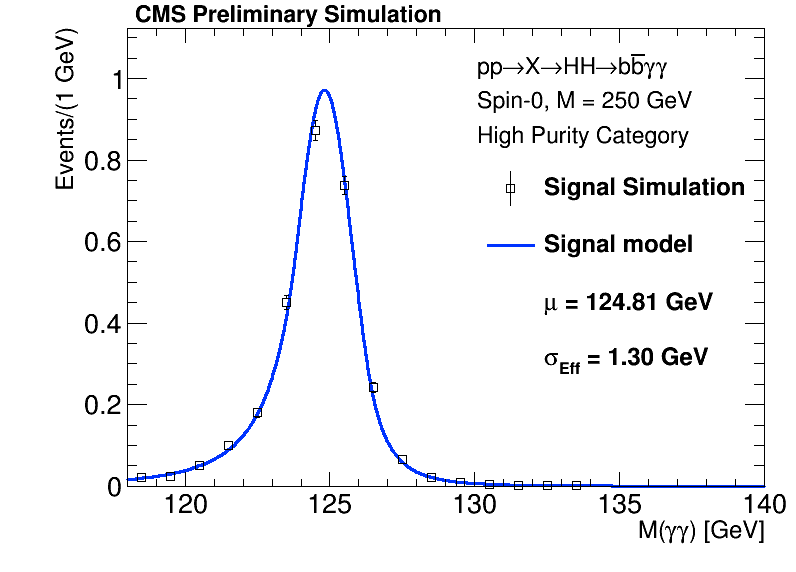
\includegraphics[width=0.45\textwidth]{figures/sec-signals/Rad250_signal_fit_mgg_cat0}\hfil
%  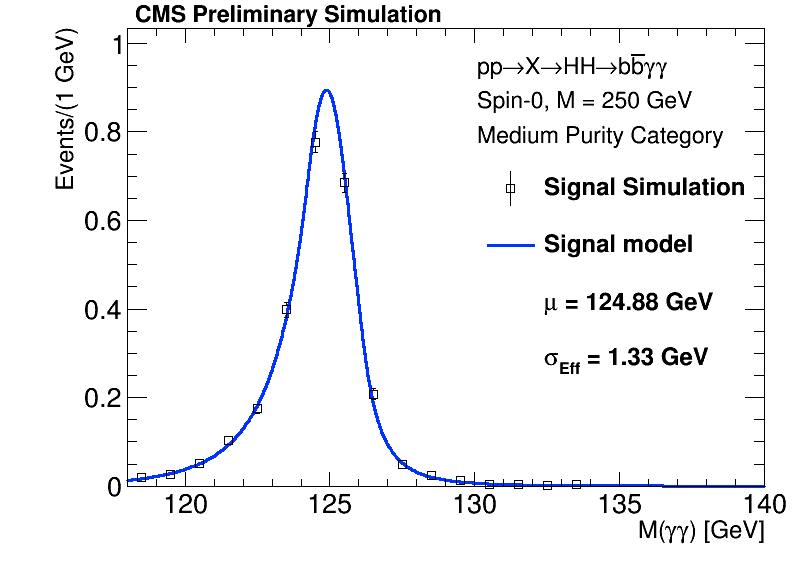
\includegraphics[width=0.45\textwidth]{figures/sec-signals/Rad250_signal_fit_mgg_cat1}\hfil
%  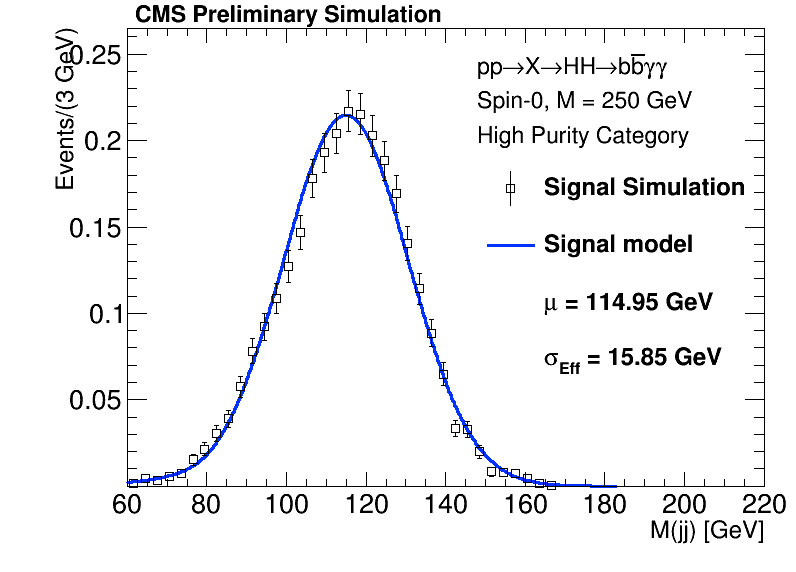
\includegraphics[width=0.45\textwidth]{figures/sec-signals/Rad250_signal_fit_mjj_cat0}\hfil
%  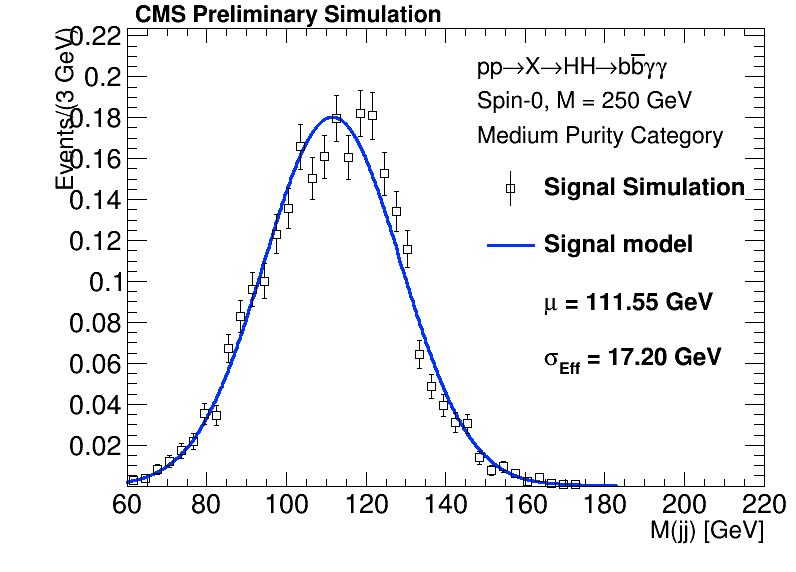
\includegraphics[width=0.45\textwidth]{figures/sec-signals/Rad250_signal_fit_mjj_cat1}\hfil
%  \caption{Signal fits for the Radion 250 GeV sample after full analysis selection, in High and Medium purity categories.}
%  \label{fig:rad250}
%\end{figure*}

\begin{figure*}[h]
  \centering
  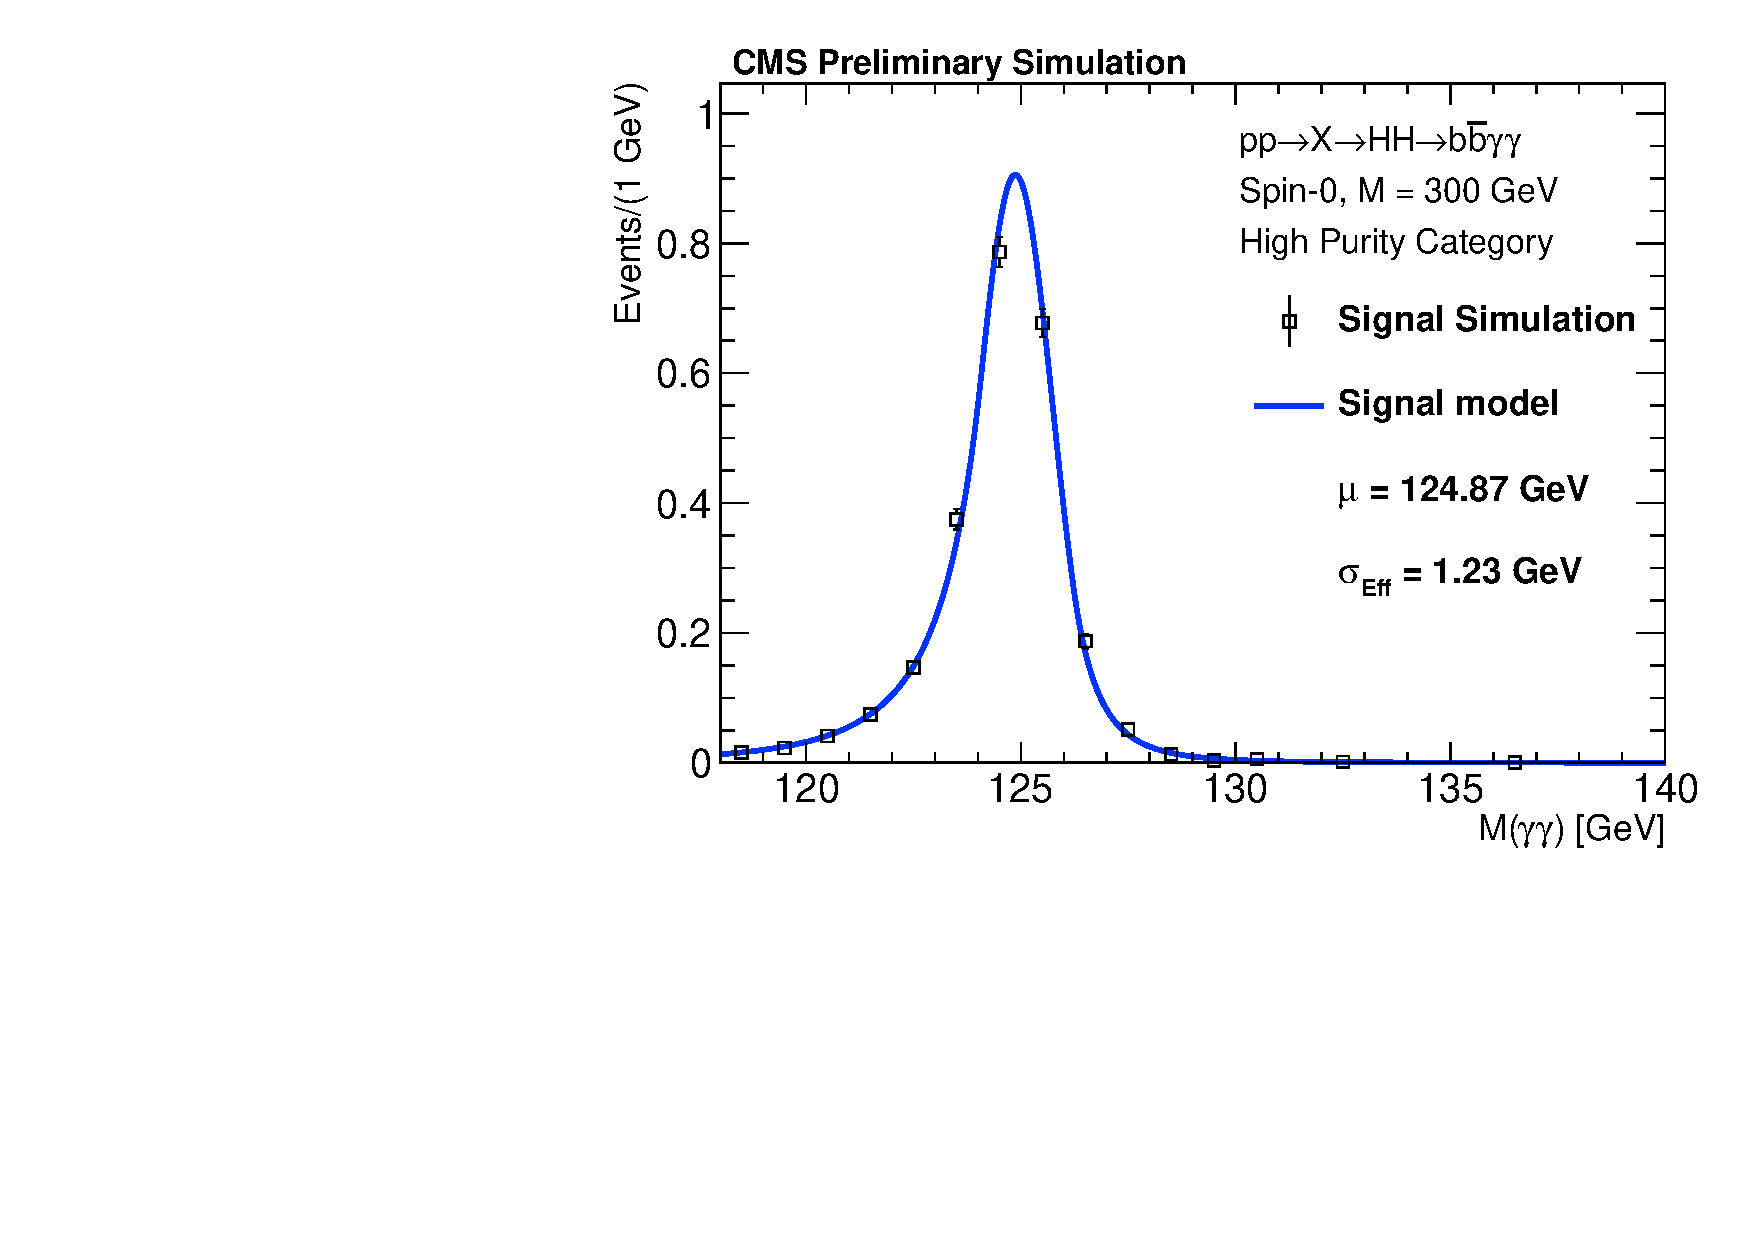
\includegraphics[width=0.45\textwidth]{figures/sec-signals/Rad300_signal_fit_mgg_cat0}\hfil
  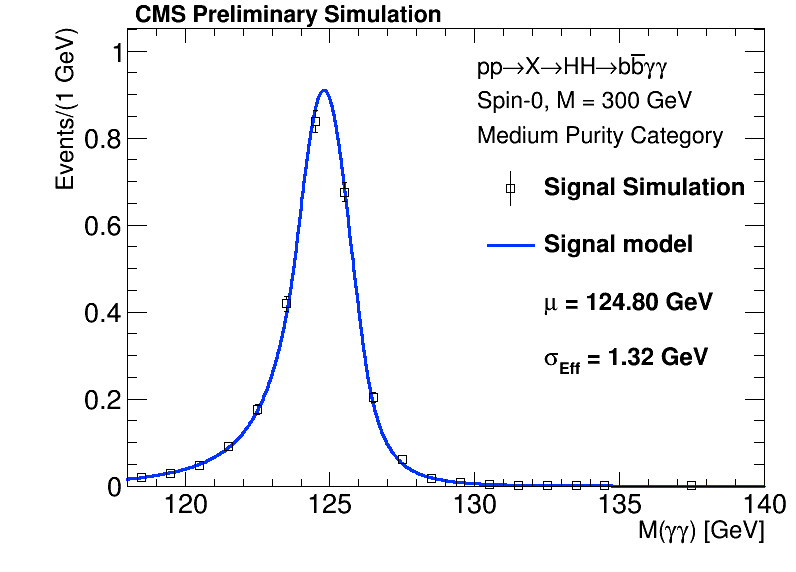
\includegraphics[width=0.45\textwidth]{figures/sec-signals/Rad300_signal_fit_mgg_cat1}\hfil
  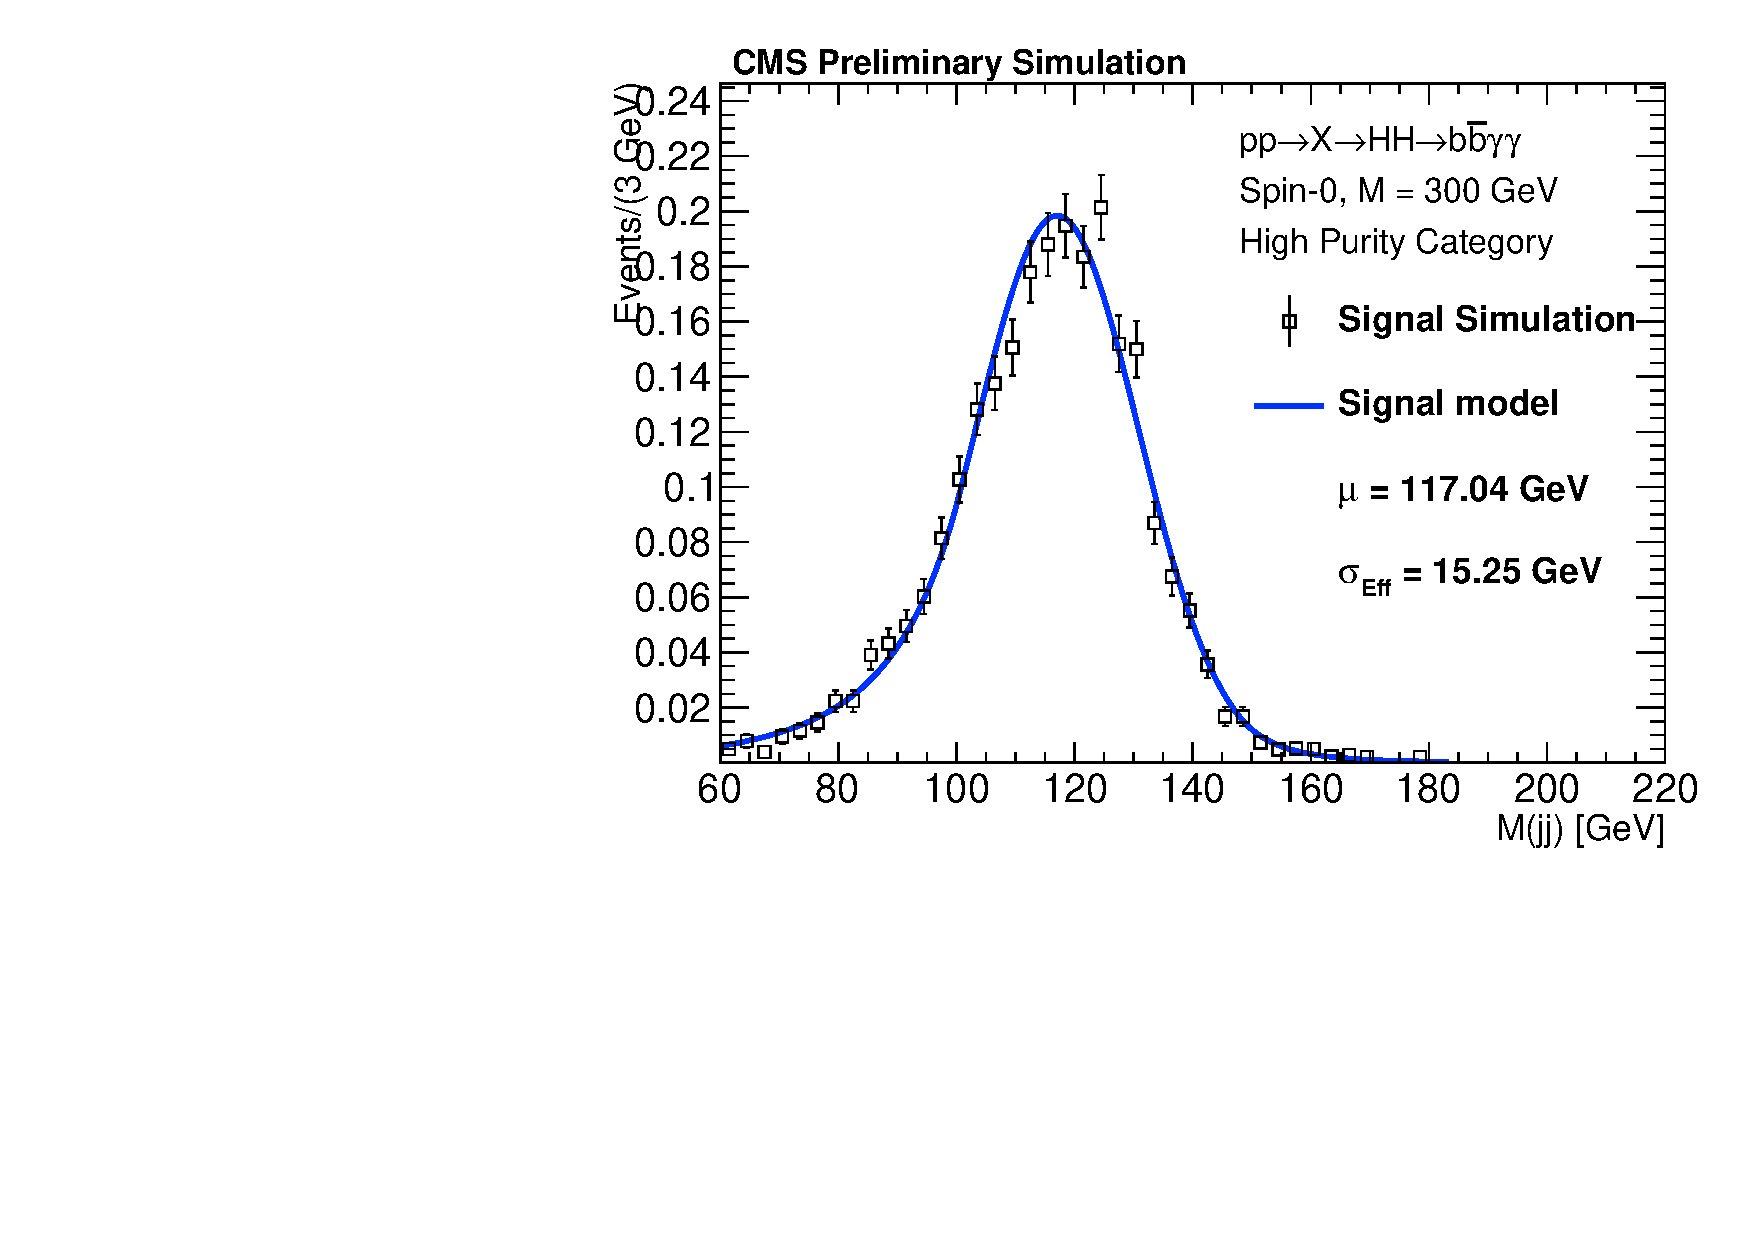
\includegraphics[width=0.45\textwidth]{figures/sec-signals/Rad300_signal_fit_mjj_cat0}\hfil
  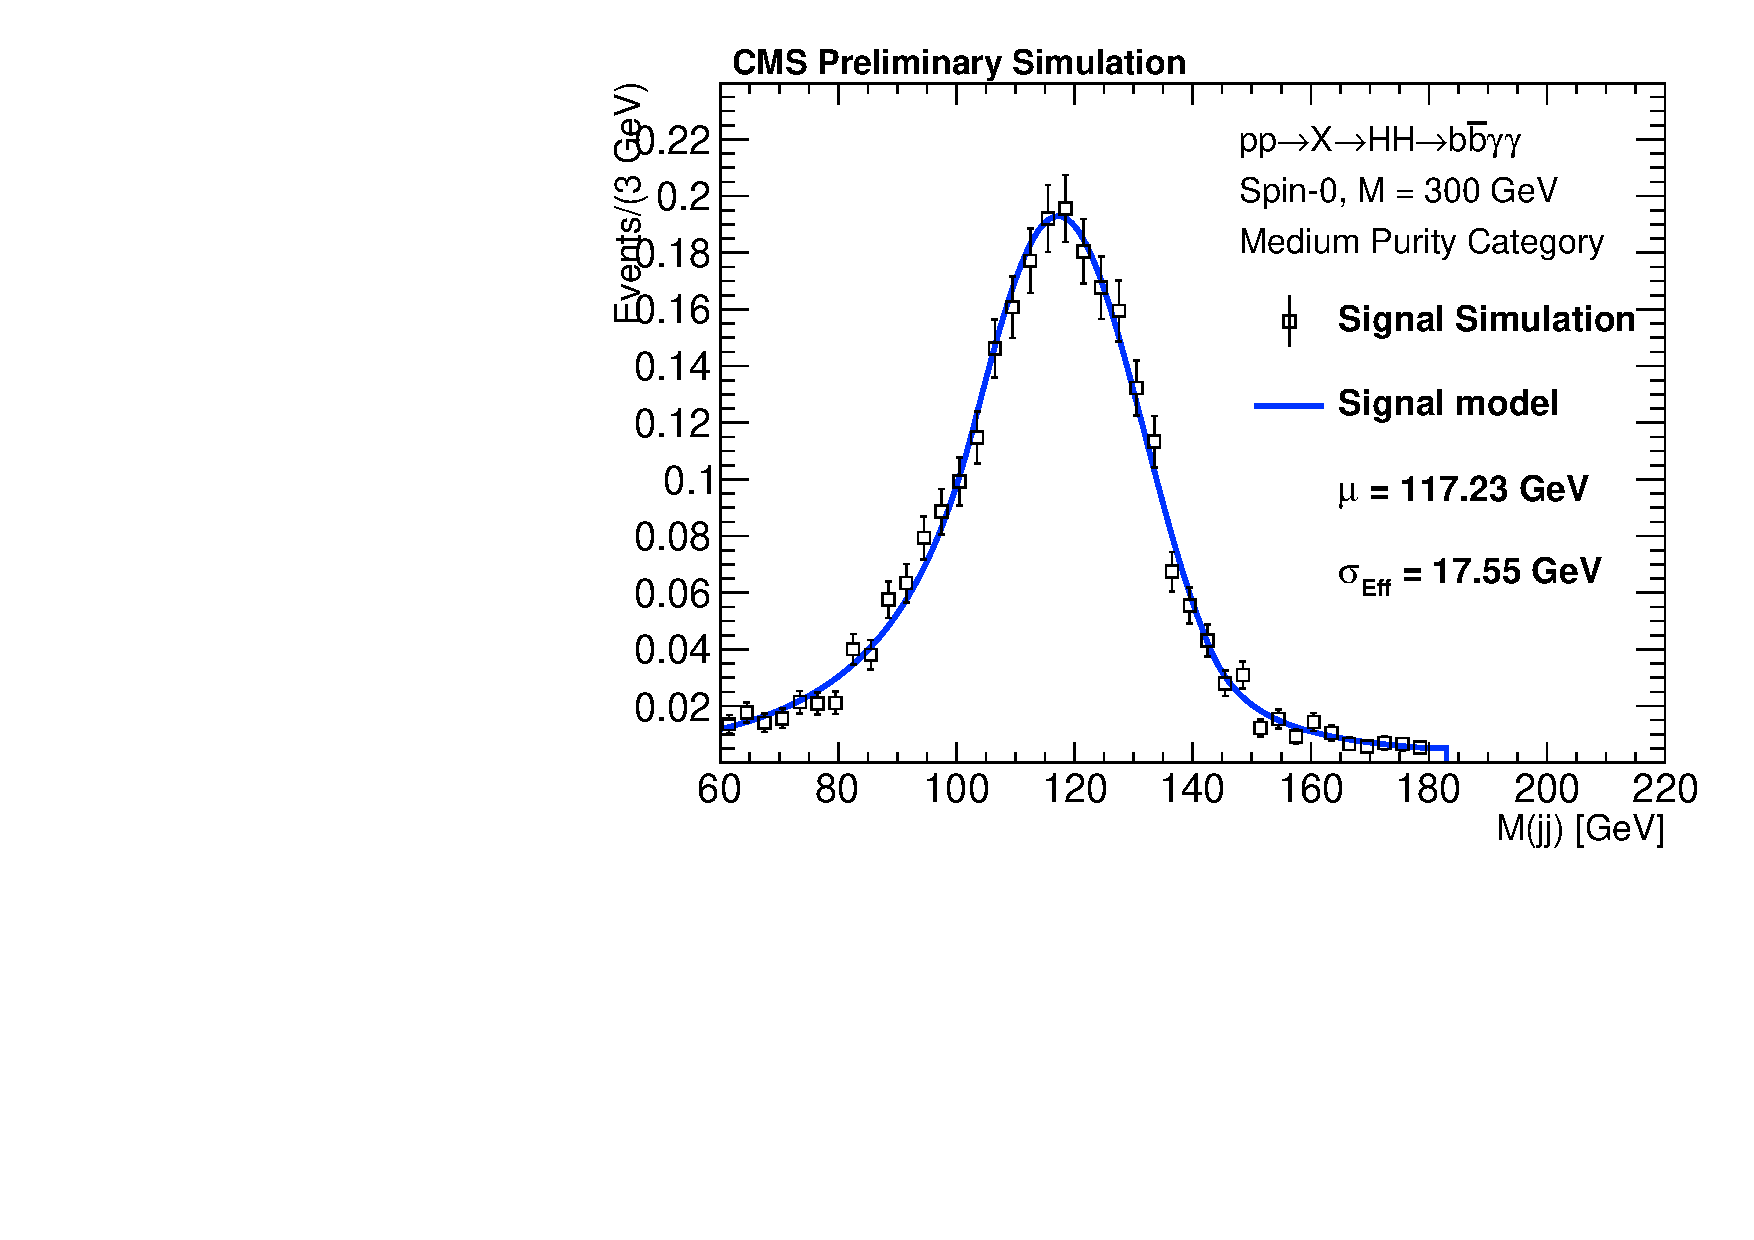
\includegraphics[width=0.45\textwidth]{figures/sec-signals/Rad300_signal_fit_mjj_cat1}\hfil
  \caption{Signal fits for the radion 300 GeV mass sample after full analysis selection, in High (left) and Medium (right) purity categories. Top plots: $\Mgg$. Bottom plots: $\Mjj$.}
  \label{fig:rad300}
\end{figure*}

%\begin{figure*}[h]
%  \centering
%  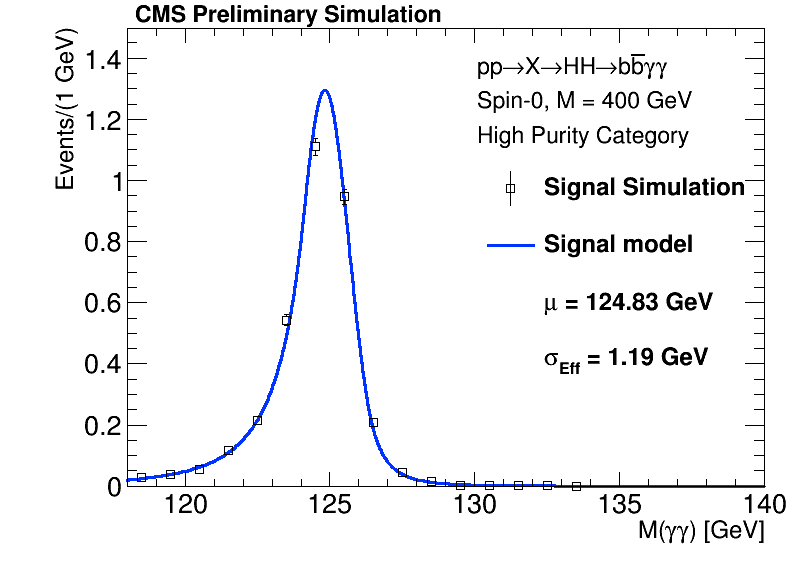
\includegraphics[width=0.45\textwidth]{figures/sec-signals/Rad400_signal_fit_mgg_cat0}\hfil
%  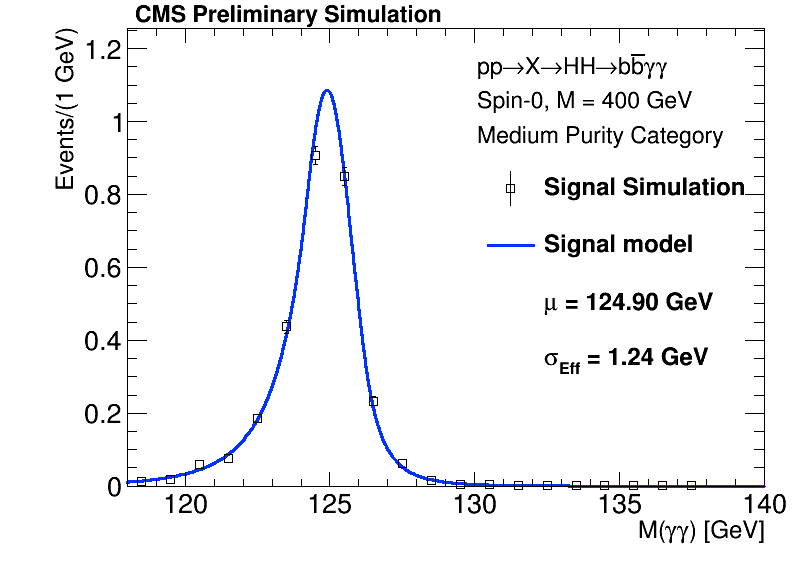
\includegraphics[width=0.45\textwidth]{figures/sec-signals/Rad400_signal_fit_mgg_cat1}\hfil
%  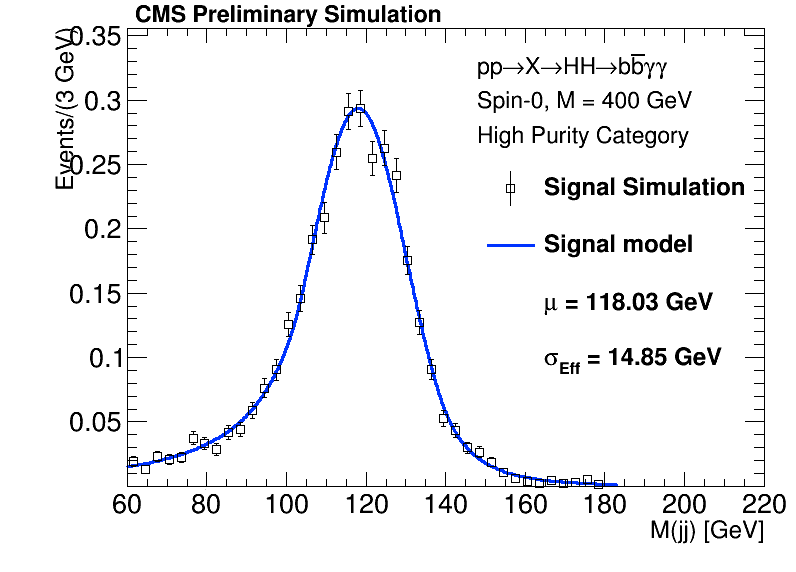
\includegraphics[width=0.45\textwidth]{figures/sec-signals/Rad400_signal_fit_mjj_cat0}\hfil
%  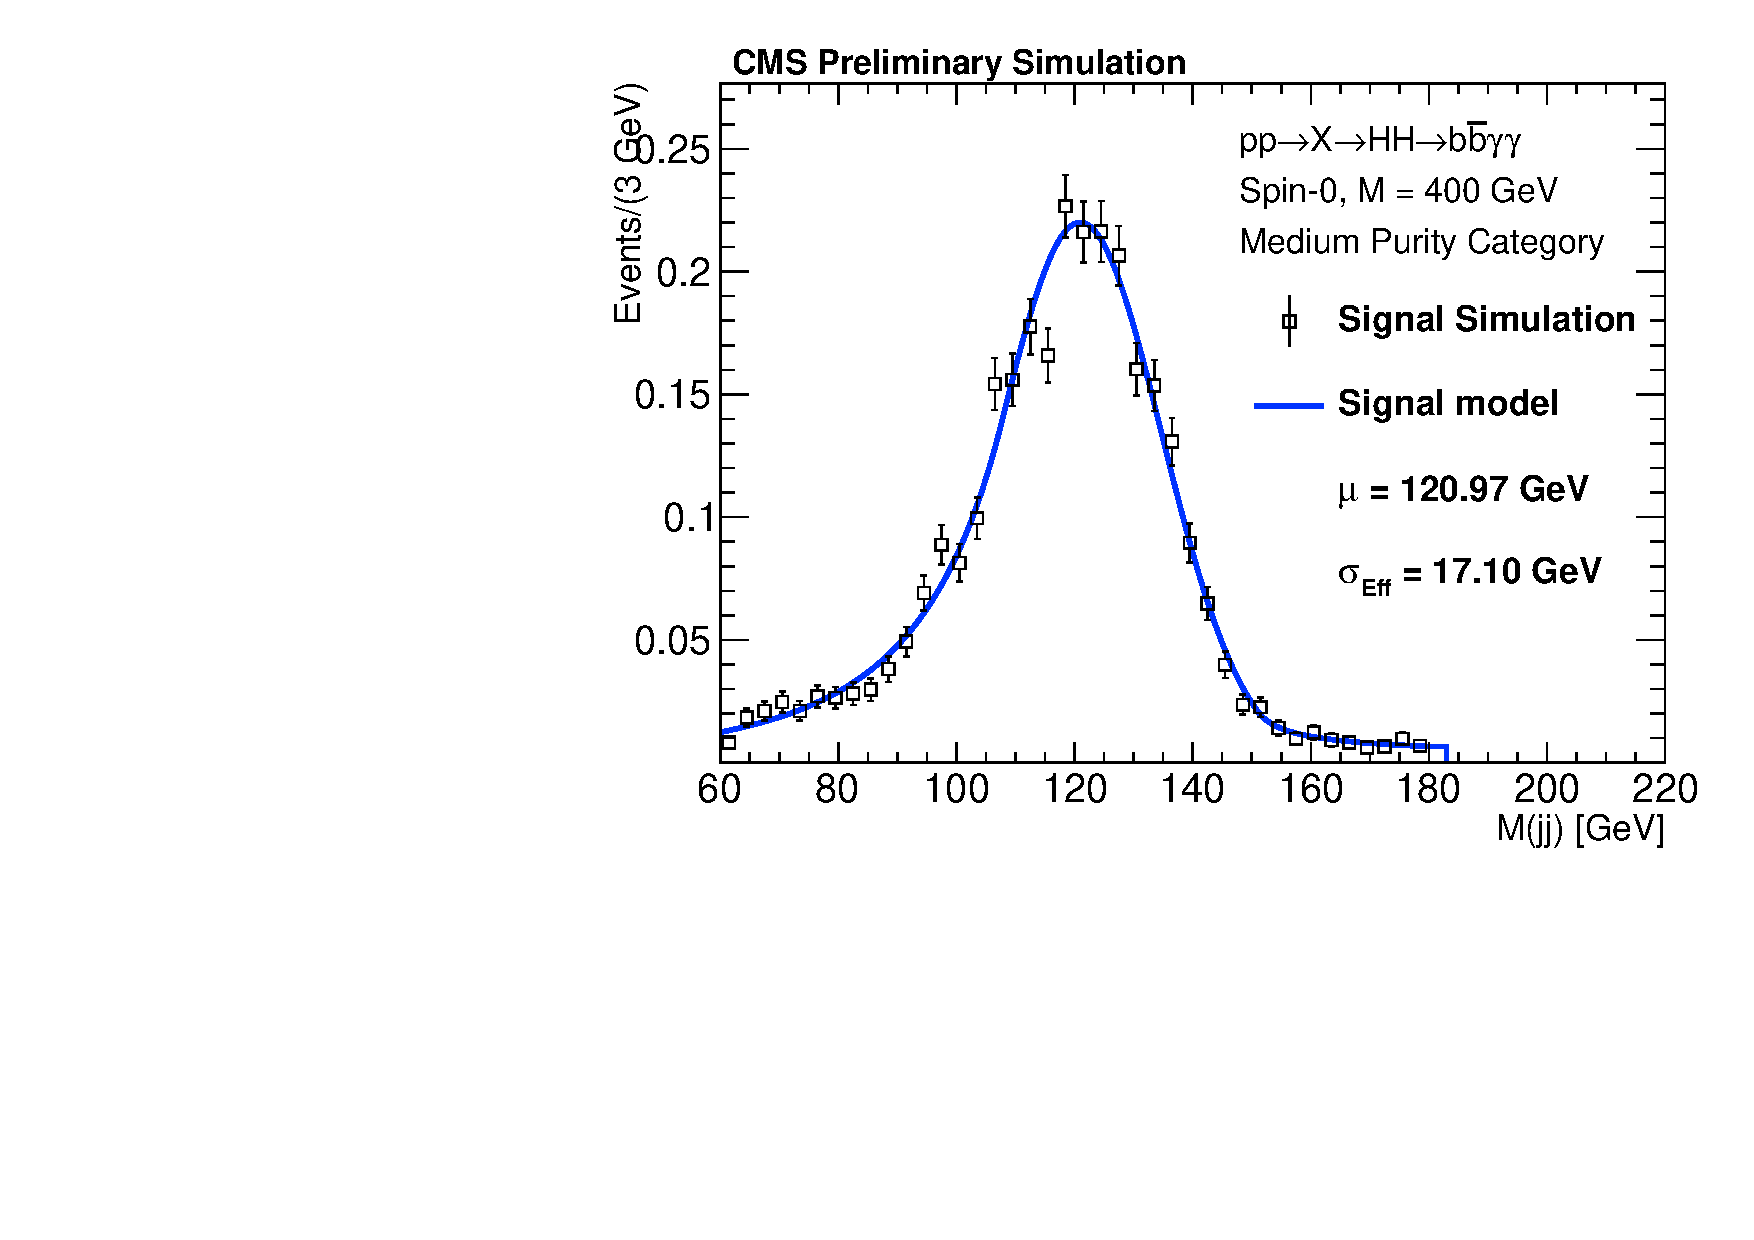
\includegraphics[width=0.45\textwidth]{figures/sec-signals/Rad400_signal_fit_mjj_cat1}\hfil
%  \caption{Signal fits for the Radion 400 GeV sample after full analysis selection, in High and Medium purity categories.}
%  \label{fig:rad400}
%\end{figure*}


\begin{figure*}[h]
  \centering
  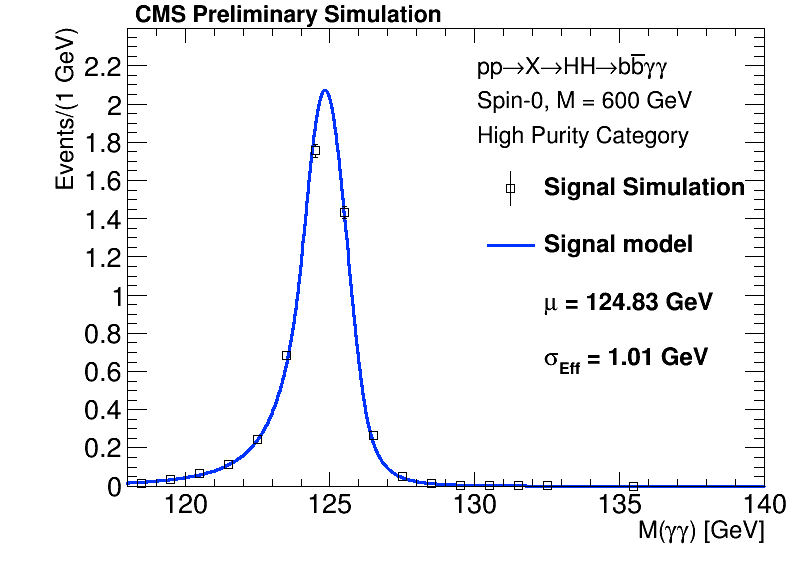
\includegraphics[width=0.45\textwidth]{figures/sec-signals/Rad600_signal_fit_mgg_cat0}\hfil
  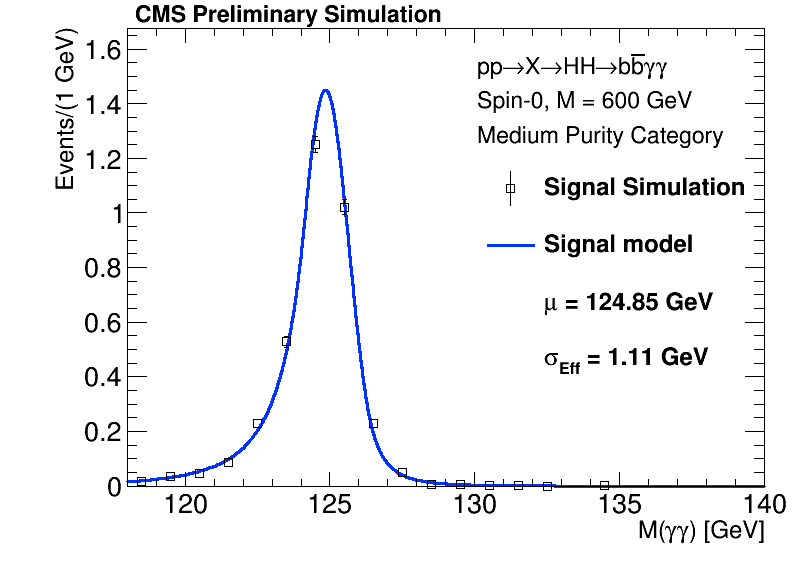
\includegraphics[width=0.45\textwidth]{figures/sec-signals/Rad600_signal_fit_mgg_cat1}\hfil
  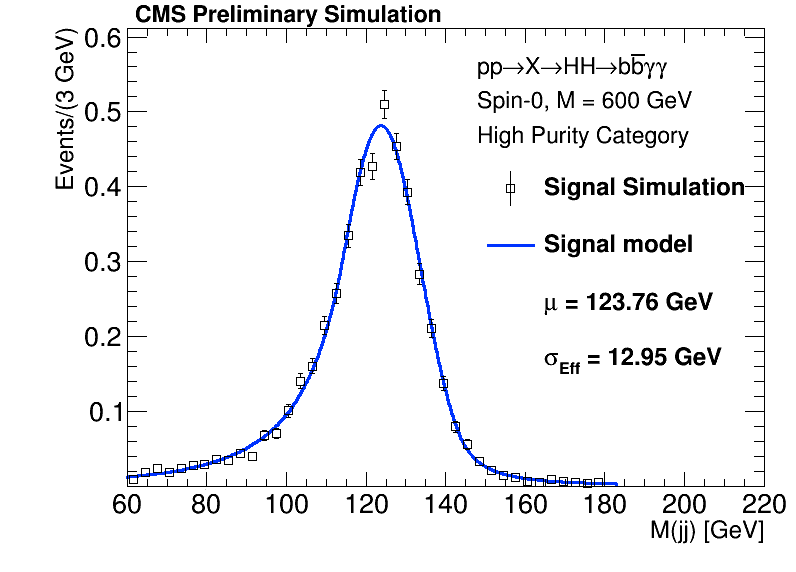
\includegraphics[width=0.45\textwidth]{figures/sec-signals/Rad600_signal_fit_mjj_cat0}\hfil
  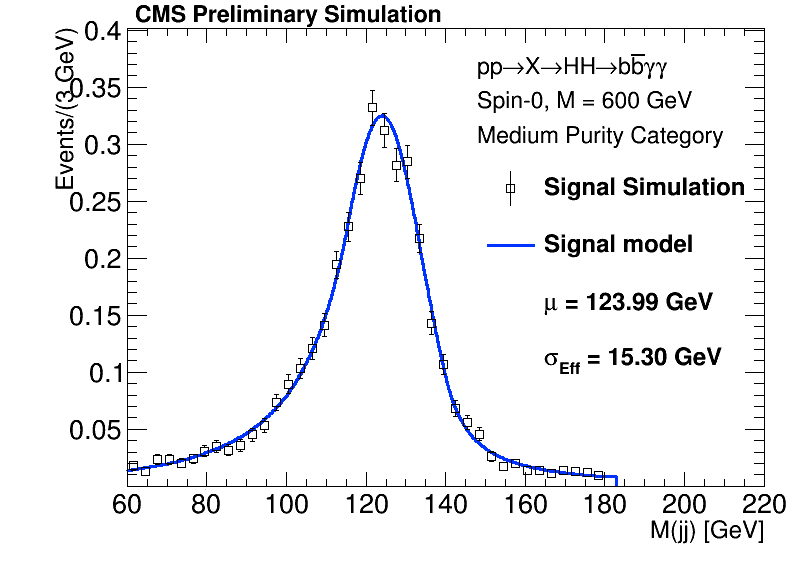
\includegraphics[width=0.45\textwidth]{figures/sec-signals/Rad600_signal_fit_mjj_cat1}\hfil
  \caption{Signal fits for the Radion 600 GeV mass sample after full analysis selection, in High (left) and Medium (right) purity categories. Top plots: $\Mgg$. Bottom plots: $\Mjj$.}
  \label{fig:rad600}
\end{figure*}

%\begin{figure*}[h]
%  \centering
%  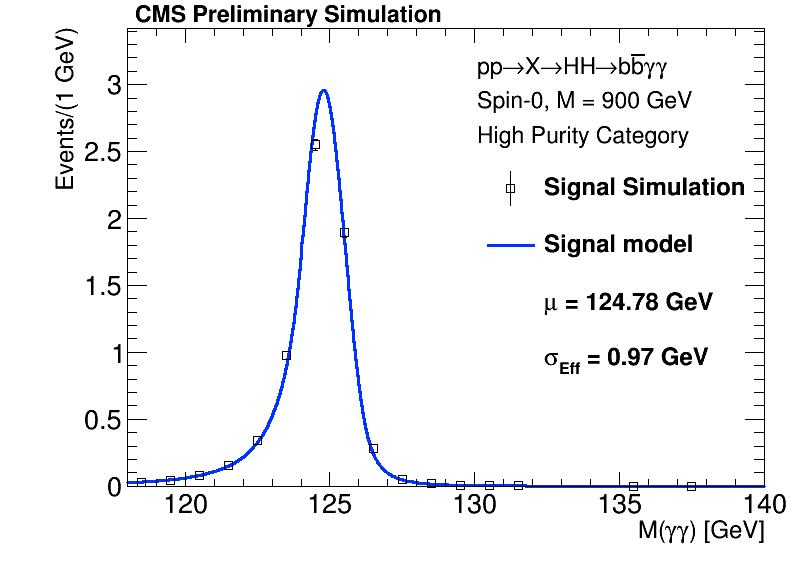
\includegraphics[width=0.45\textwidth]{figures/sec-signals/Rad900_signal_fit_mgg_cat0}\hfil
%  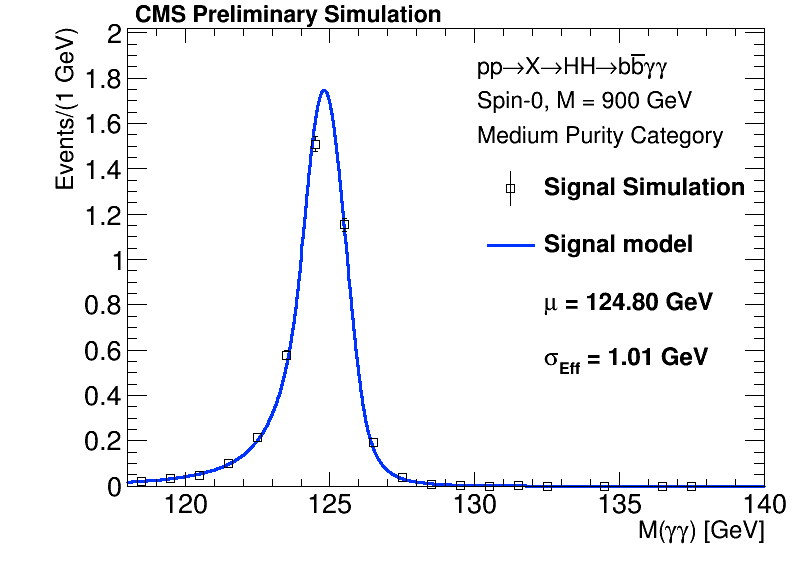
\includegraphics[width=0.45\textwidth]{figures/sec-signals/Rad900_signal_fit_mgg_cat1}\hfil
%  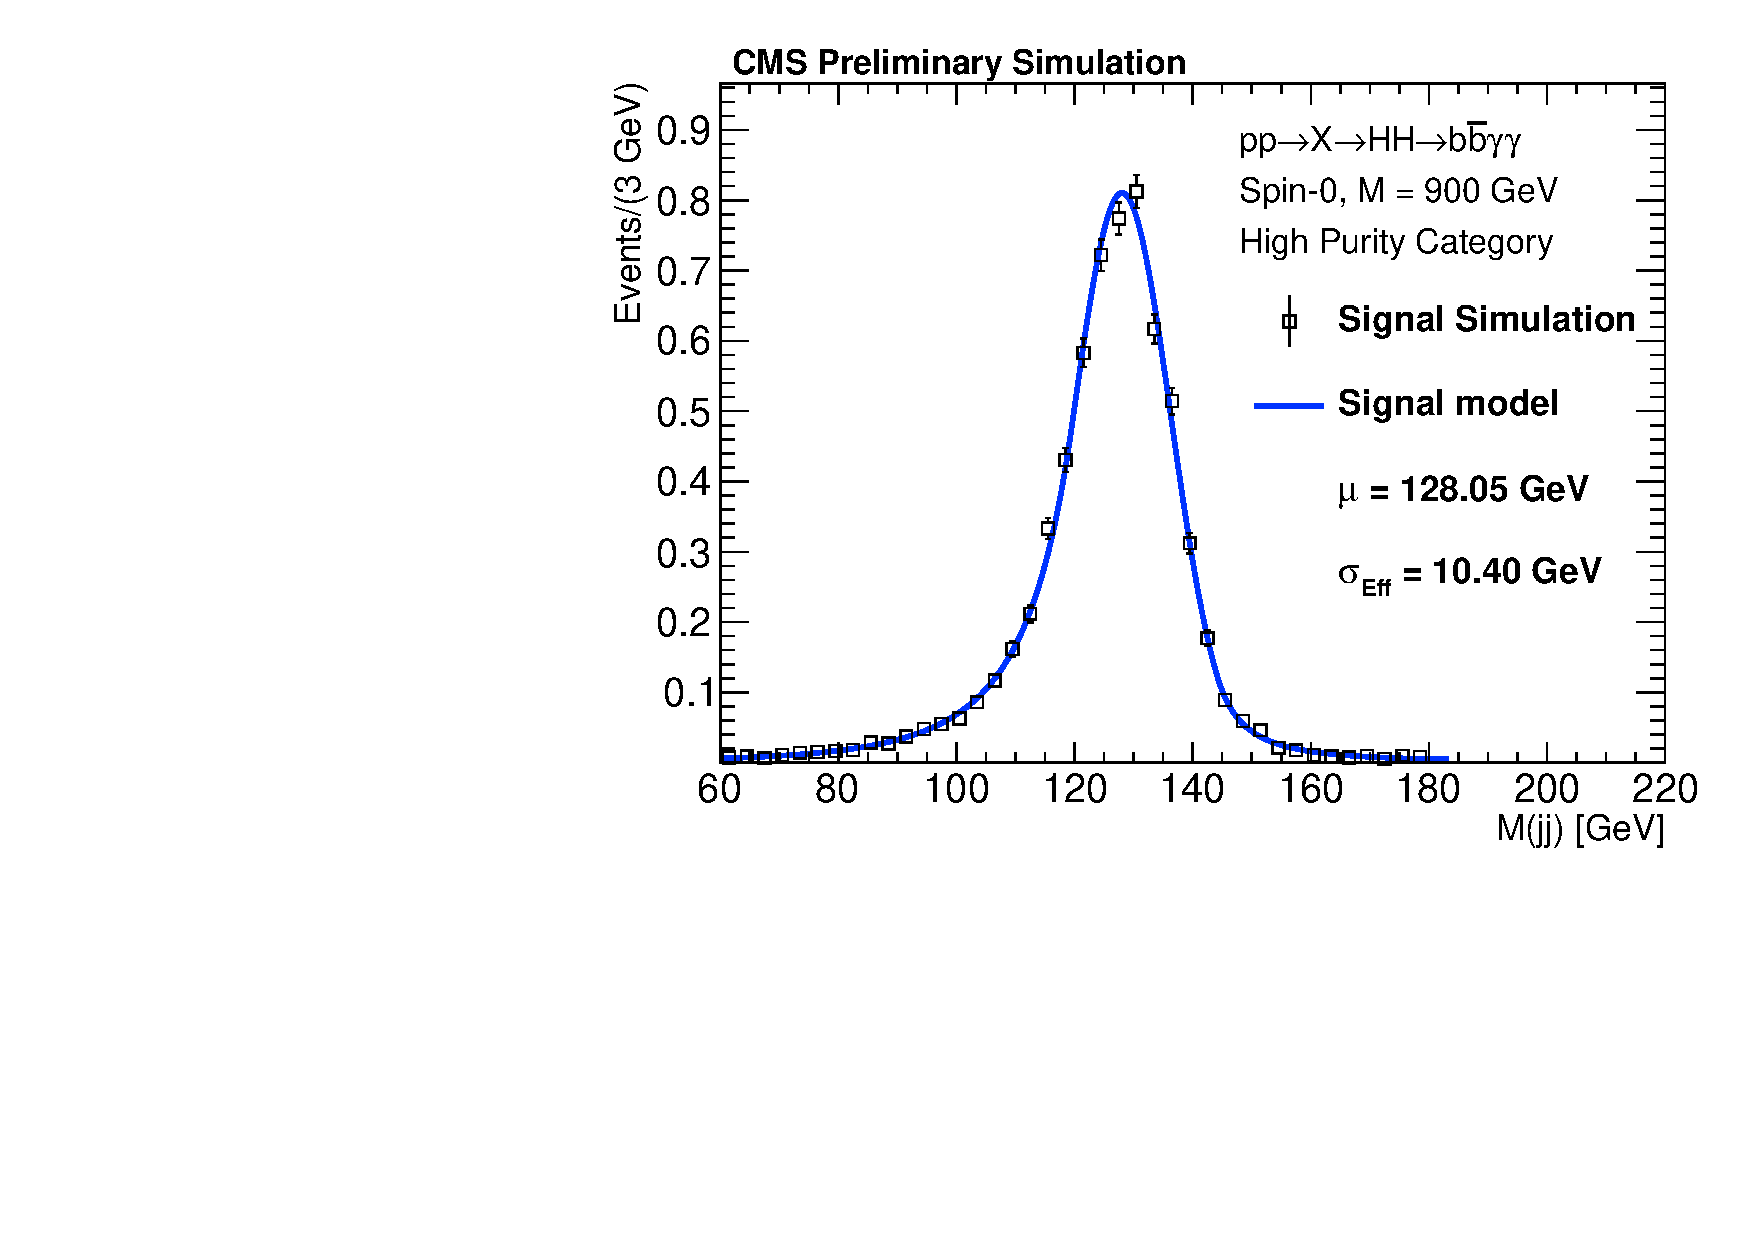
\includegraphics[width=0.45\textwidth]{figures/sec-signals/Rad900_signal_fit_mjj_cat0}\hfil
%  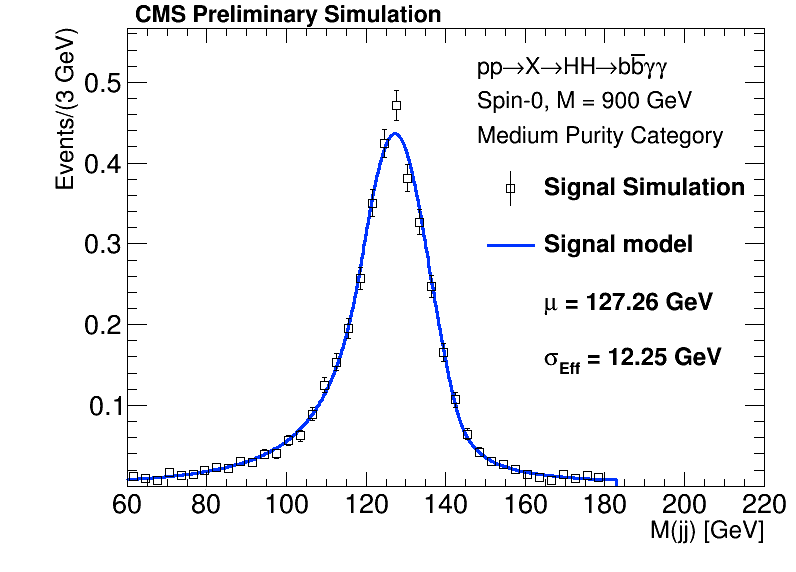
\includegraphics[width=0.45\textwidth]{figures/sec-signals/Rad900_signal_fit_mjj_cat1}\hfil
%  \caption{Signal fits for the Radion 900 GeV sample after full analysis selection, in High and Medium purity categories.}
%  \label{fig:rad900}
%\end{figure*}


\begin{figure*}[h]
  \centering
  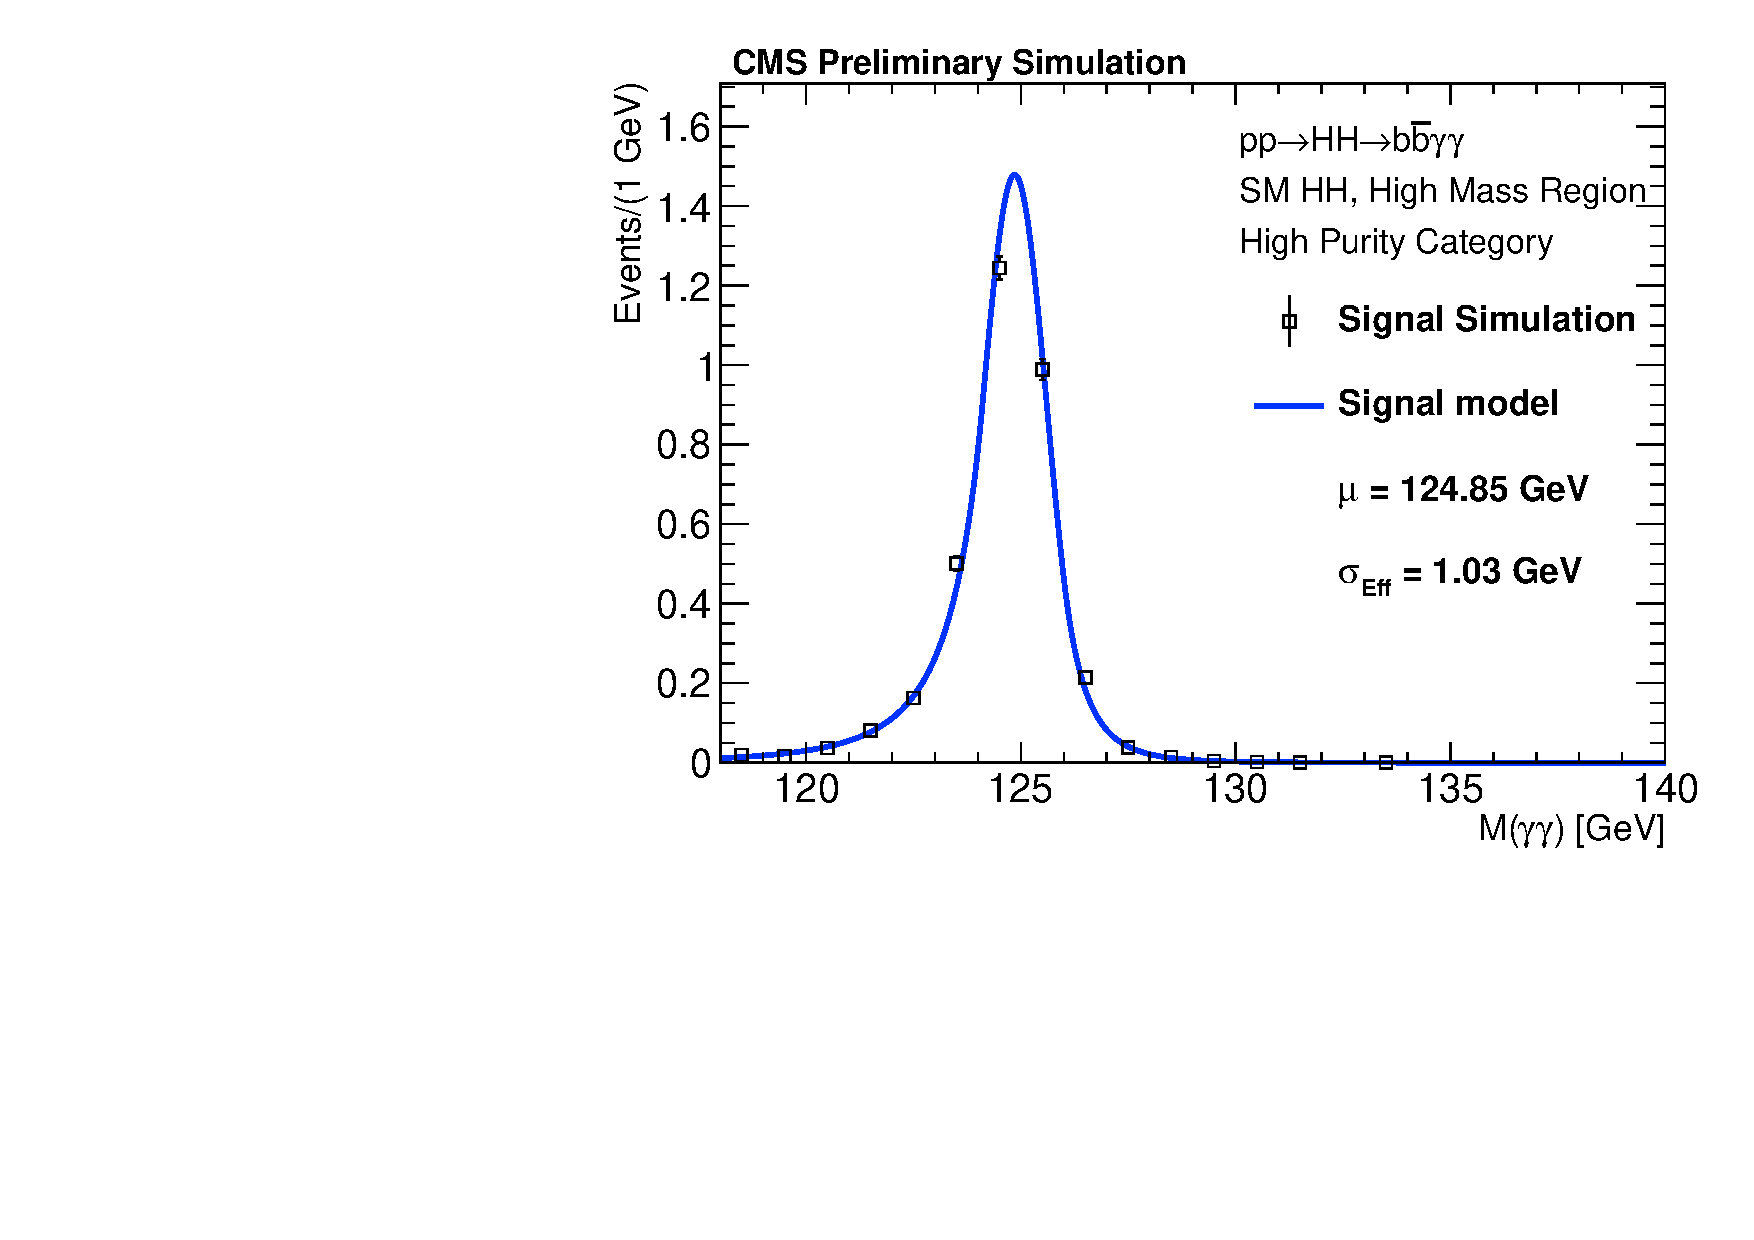
\includegraphics[width=0.45\textwidth]{figures/sec-signals/SMHM_signal_fit_mgg_cat0}\hfil
  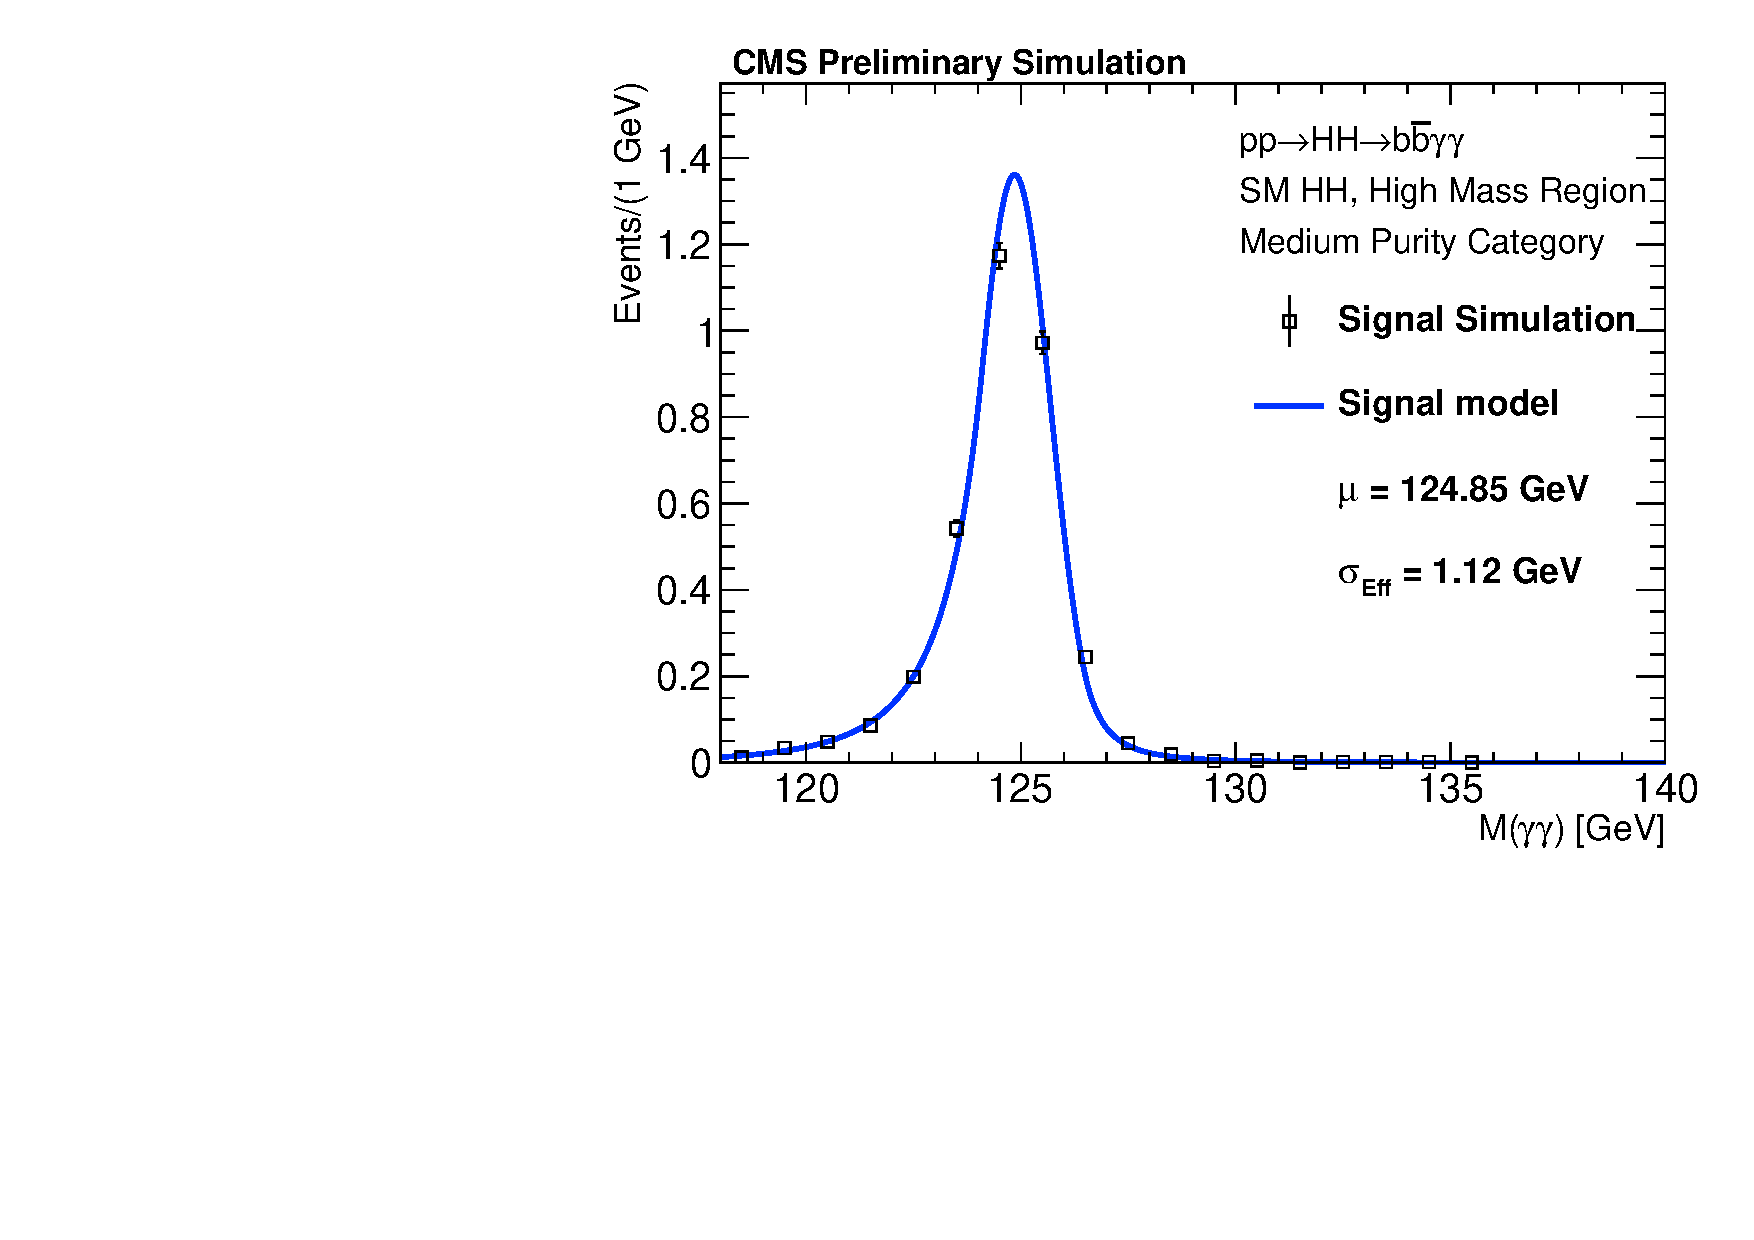
\includegraphics[width=0.45\textwidth]{figures/sec-signals/SMHM_signal_fit_mgg_cat1}\hfil
  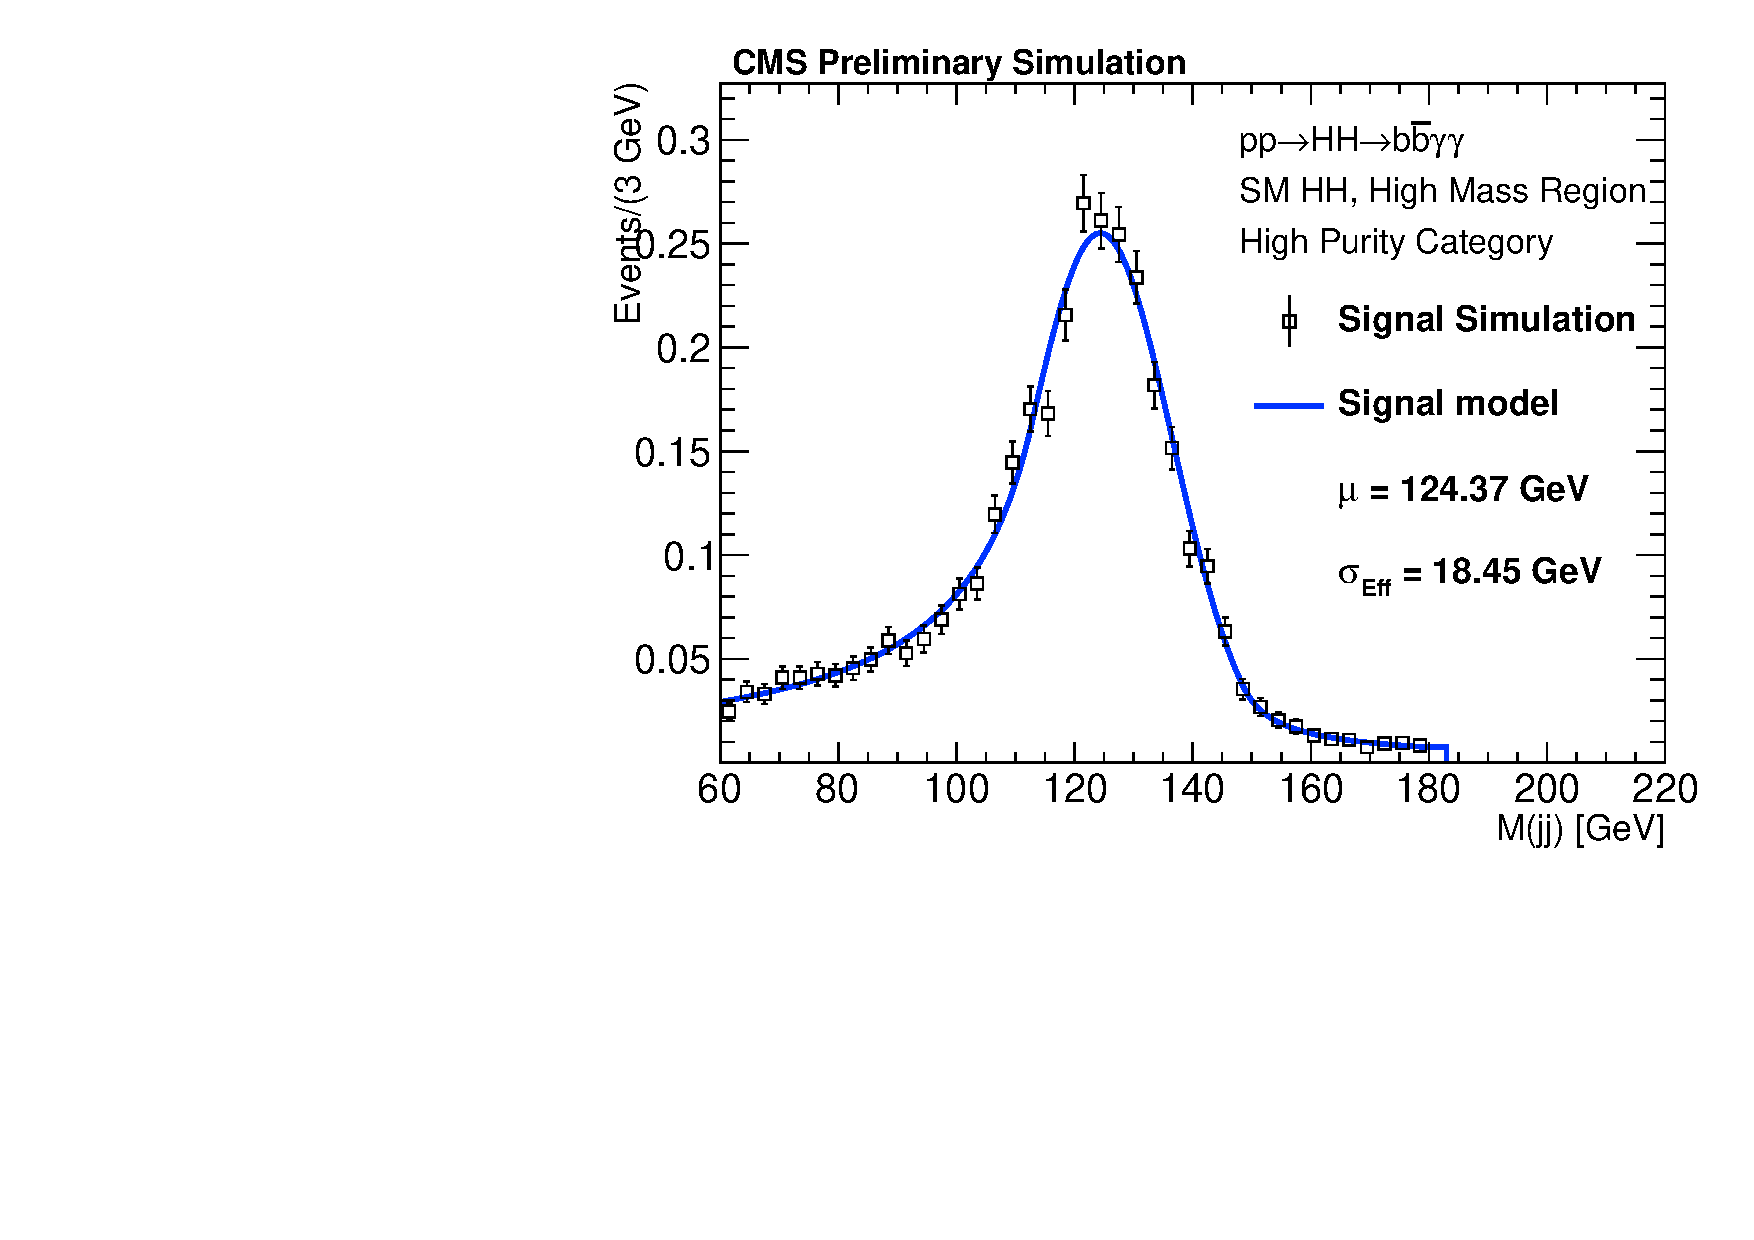
\includegraphics[width=0.45\textwidth]{figures/sec-signals/SMHM_signal_fit_mjj_cat0}\hfil
  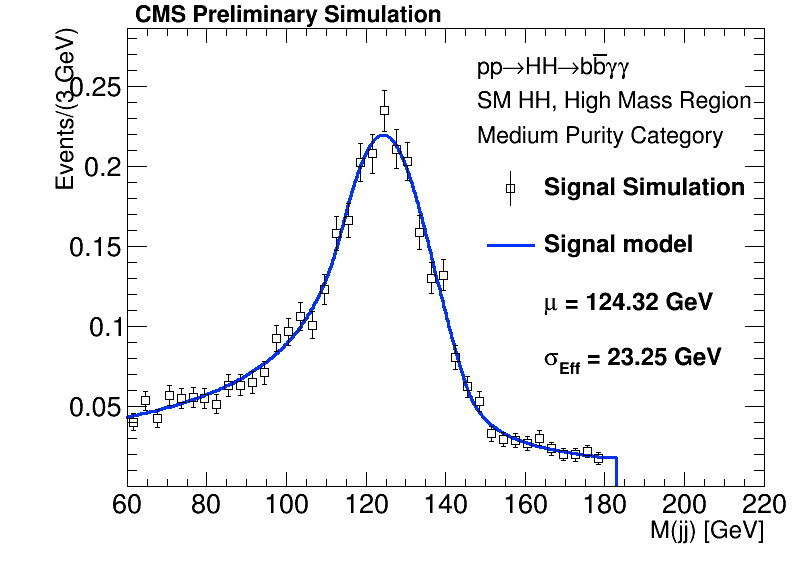
\includegraphics[width=0.45\textwidth]{figures/sec-signals/SMHM_signal_fit_mjj_cat1}\hfil
  \caption{Signal fits for the SM HH non-resonant sample after full analysis selection, in High (left) and Medium (right) purity categories. Top plots: $\Mgg$. Bottom plots: $\Mjj$.}
  \label{fig:sig_highmassSM}
\end{figure*}

\begin{figure*}[h]
  \centering
  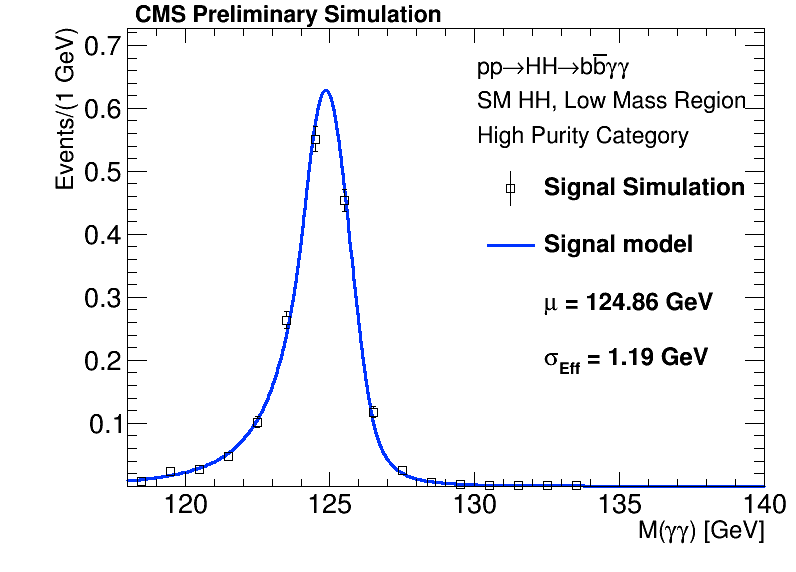
\includegraphics[width=0.45\textwidth]{figures/sec-signals/SMLM_signal_fit_mgg_cat0}\hfil
  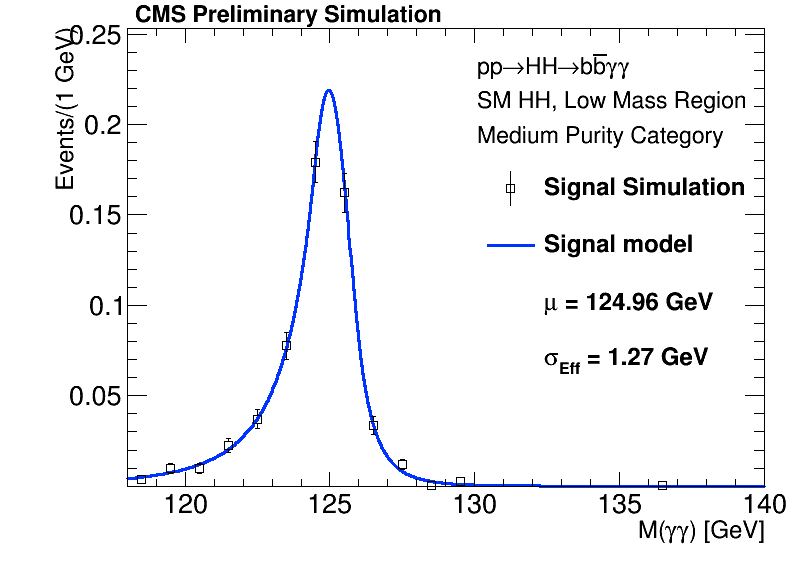
\includegraphics[width=0.45\textwidth]{figures/sec-signals/SMLM_signal_fit_mgg_cat1}\hfil
  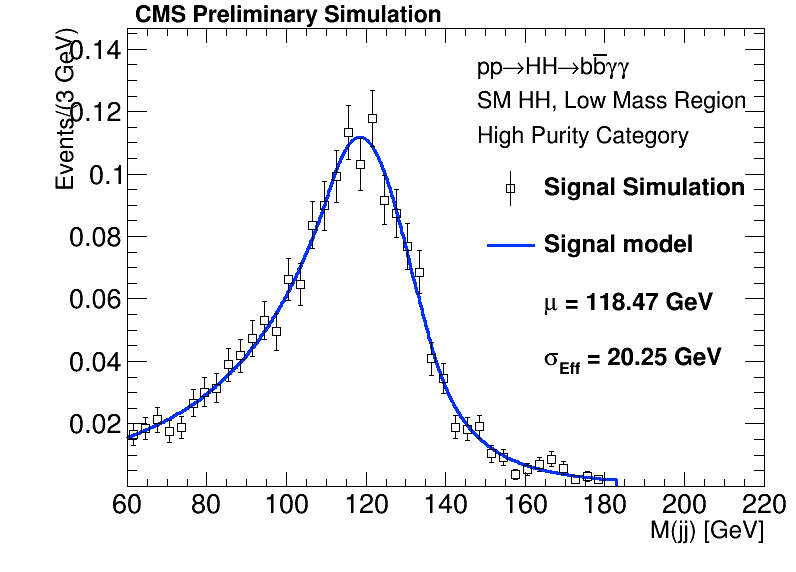
\includegraphics[width=0.45\textwidth]{figures/sec-signals/SMLM_signal_fit_mjj_cat0}\hfil
  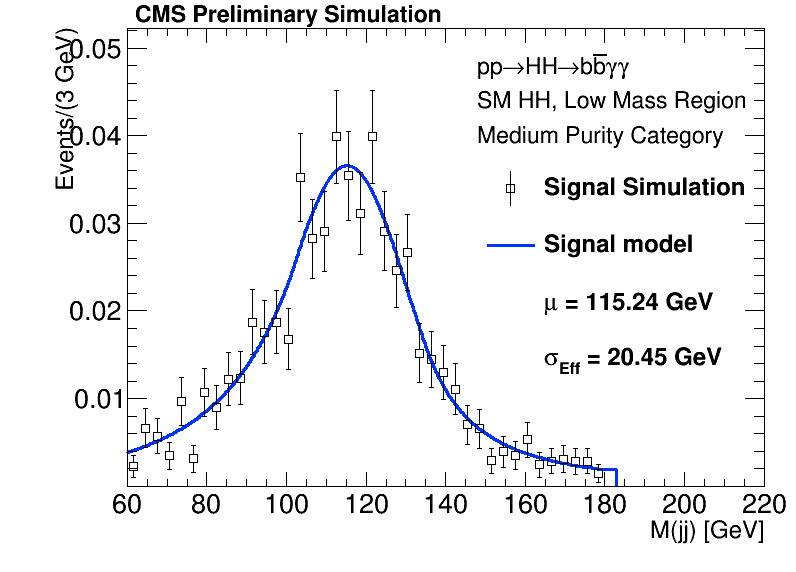
\includegraphics[width=0.45\textwidth]{figures/sec-signals/SMLM_signal_fit_mjj_cat1}\hfil
  \caption{Signal fits for the SM HH non-resonant sample after full analysis selection, in High (left) and Medium (right) purity categories. Top plots: $\Mgg$. Bottom plots: $\Mjj$.}
  \label{fig:sig_lowmassSM}
\end{figure*}

\subsubsection{Correlation Studies}

The choice of parametric signal model makes the assumption that the full 2D distribution can be modeled by a product of PDFs. 
This choice is not the most general one, as it does not model correlations between $\Mjj$ and $\Mgg$. 
One important question, therefore, is whether the analysis is sensitive to correlations that are not modeled by our choice of signal model. 
To study this, we study the differences between the MC signal simulation and the 2D fitted PDF via residuals:
\begin{equation}
R_{ij} = \frac{N^{\textrm{PDF}}_{ij} - N^{\textrm{MC}}_{ij}}{\sigma_{N^{\textrm{PDF}}_{ij}}^{\textrm{Poisson}}},
\end{equation}
where $ij$ refers to bin $i$ in $\Mgg$ and bin $j$ in $\Mjj$, and $\sigma_{N^{\textrm{PDF}}_{ij}}^{\textrm{Poisson}}$ is the Poissonian error of the expected (PDF) and observed (MC).  
These residuals are shown in Figures \ref{fig:sig_resi_hm_hpc}, \ref{fig:sig_resi_hm_mpc}, \ref{fig:sig_resi_lm_hpc} and \ref{fig:sig_resi_lm_mpc}.
The signal MC normalization for these plots are to 1/fb signal cross section. 
We see no structures in the residual plots in the region where the signal is expected. Therefore, we assume that the PDF product modeling is good enough given the statistical precision of our current dataset. 

\begin{figure*}[h]
  \centering
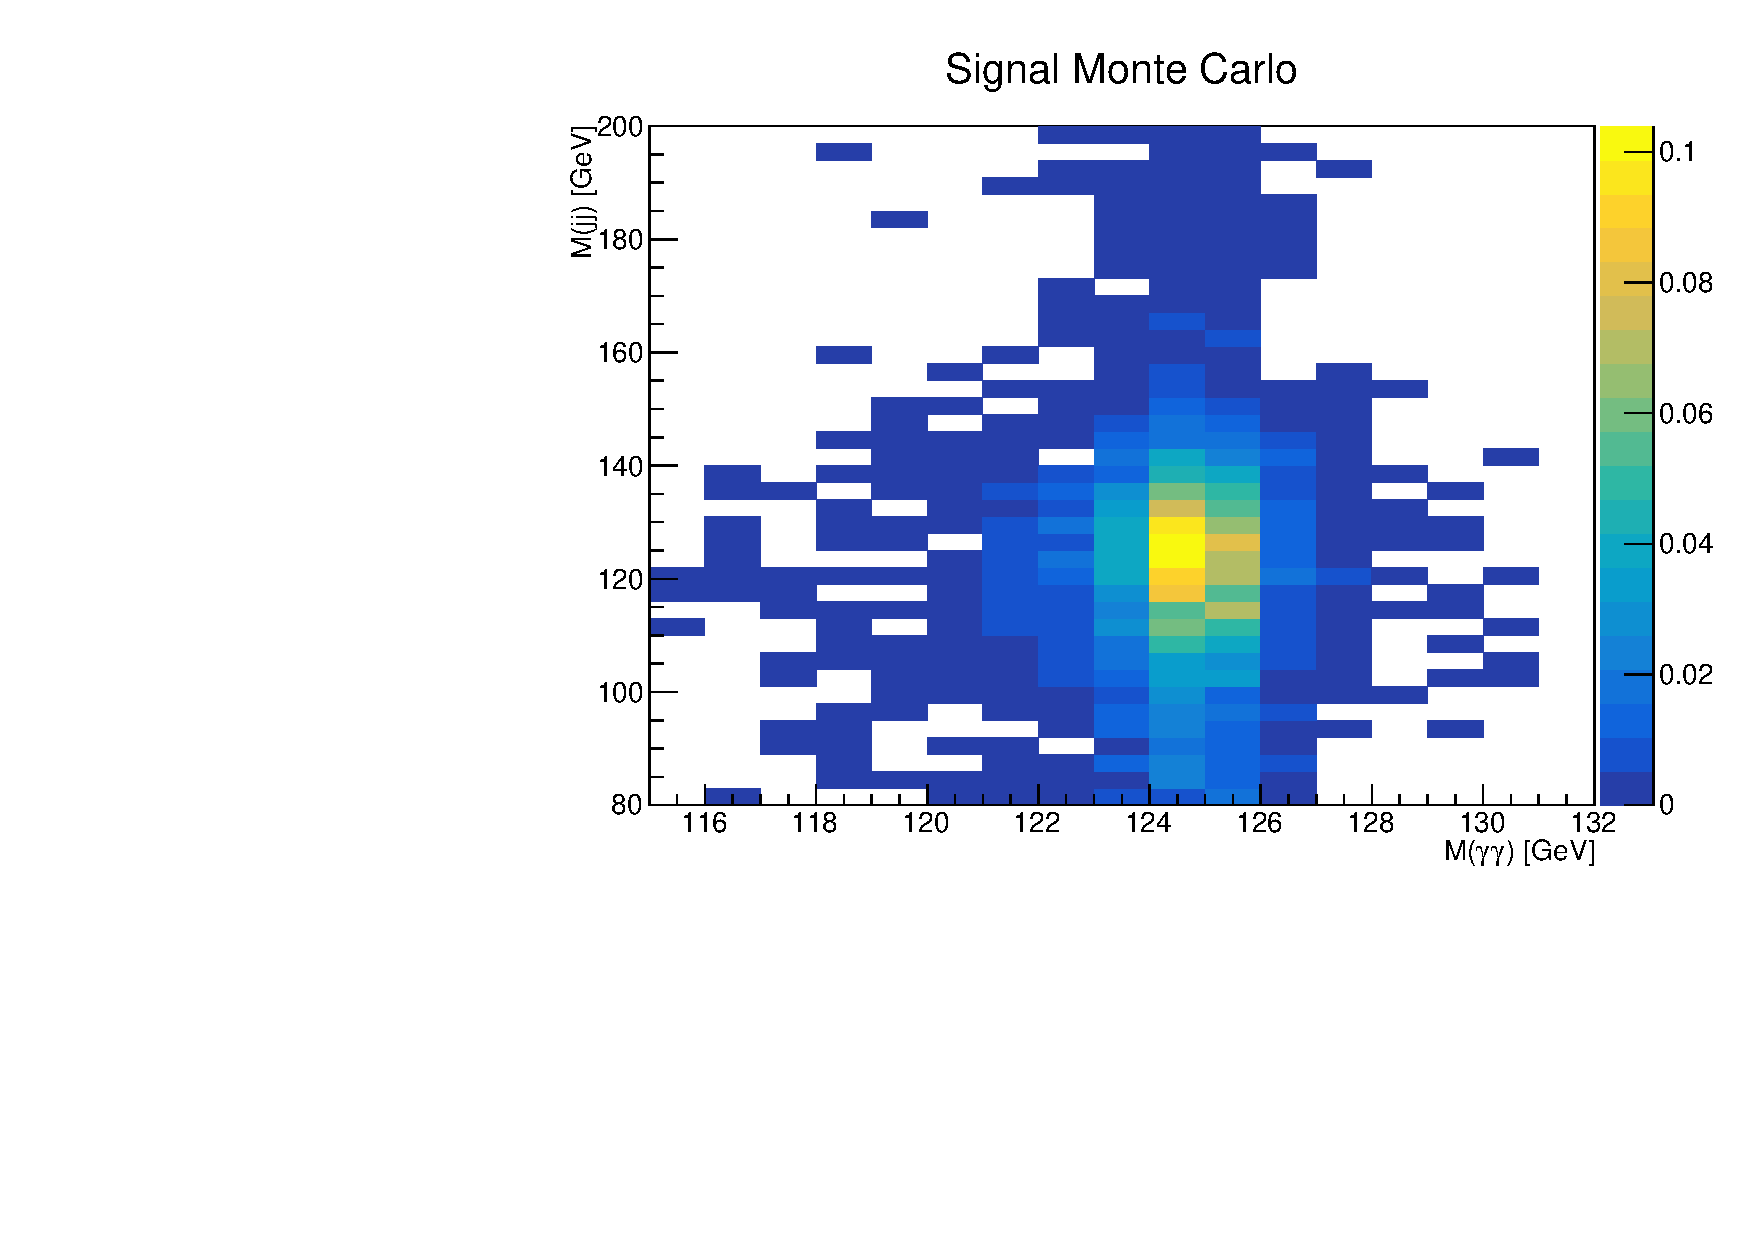
\includegraphics[width=0.3\textwidth]{figures/sec-signals/SignalResiduals/h_mc_HM_cat0}\hfil
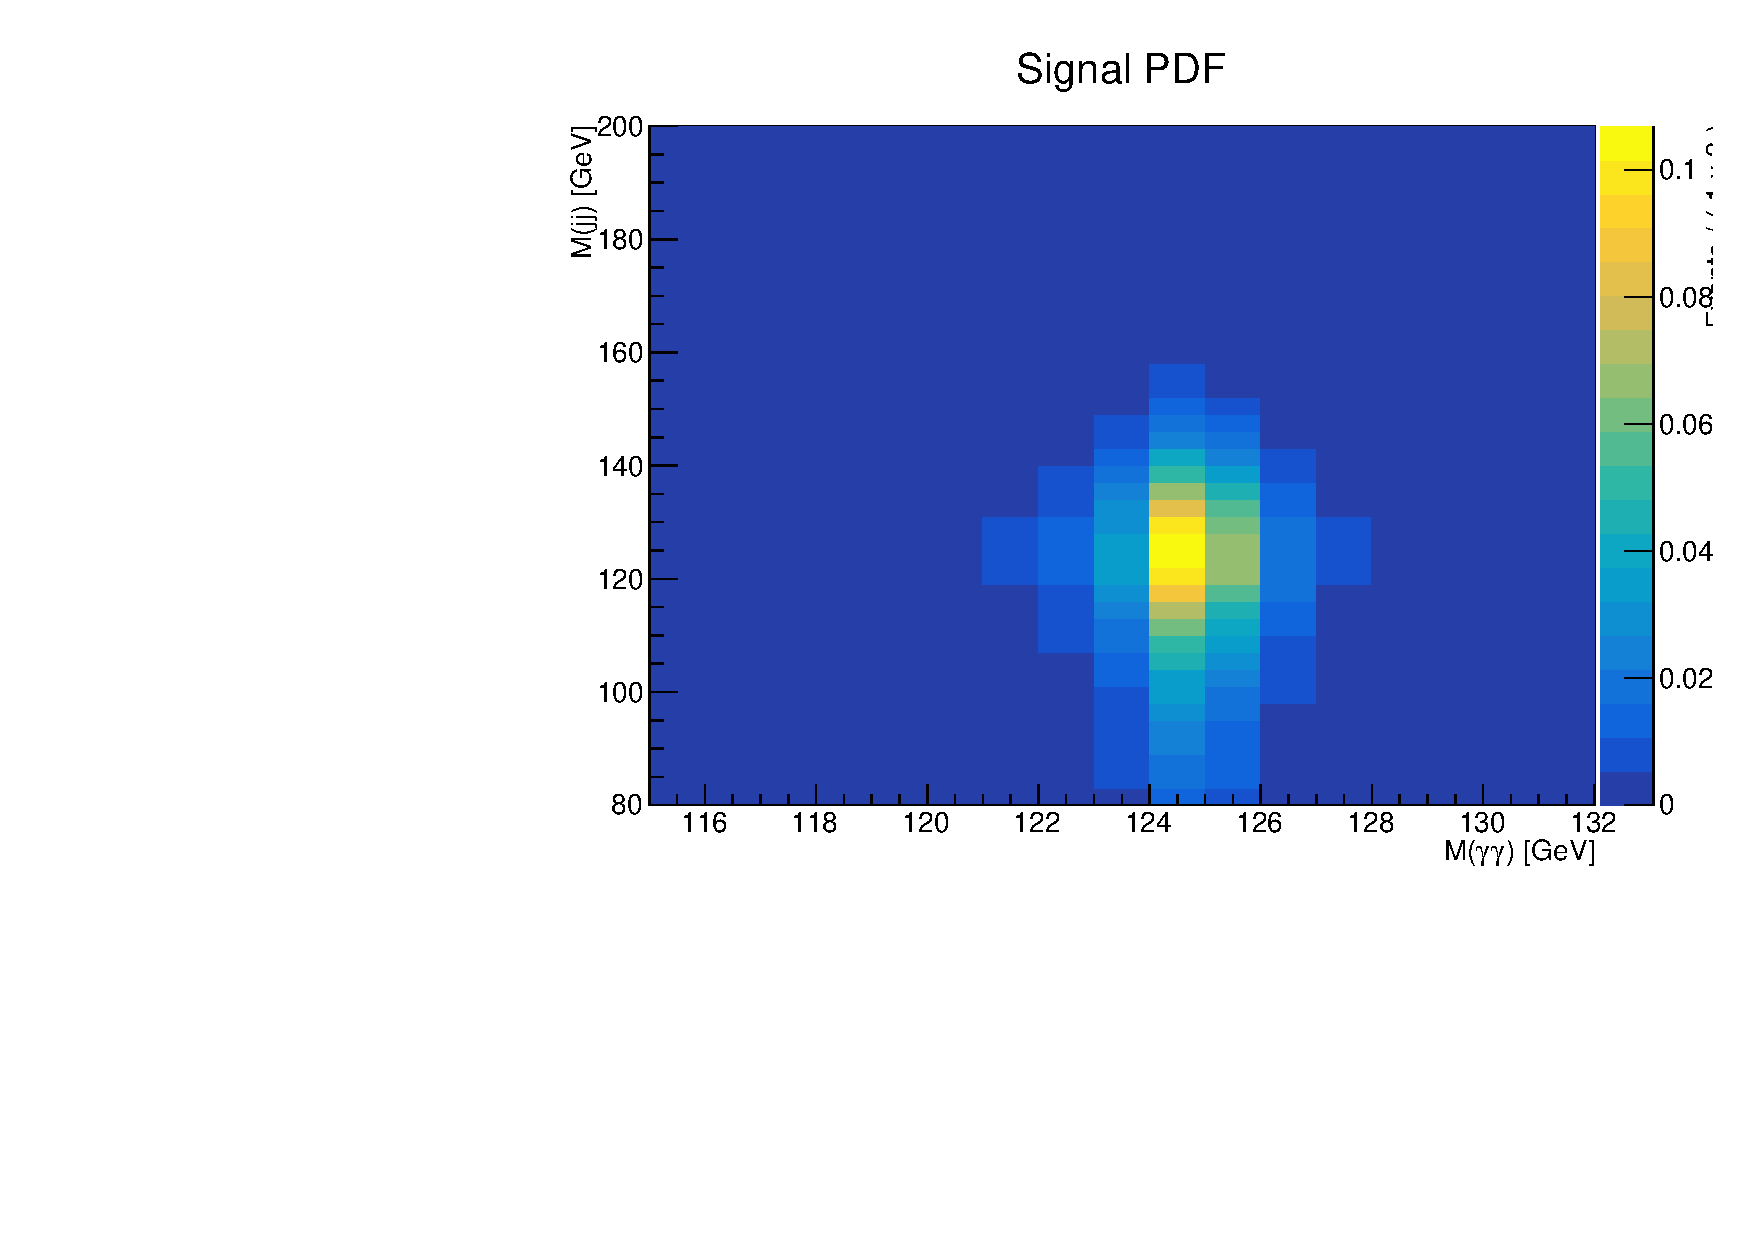
\includegraphics[width=0.3\textwidth]{figures/sec-signals/SignalResiduals/h_pd_HM_cat0}\hfil
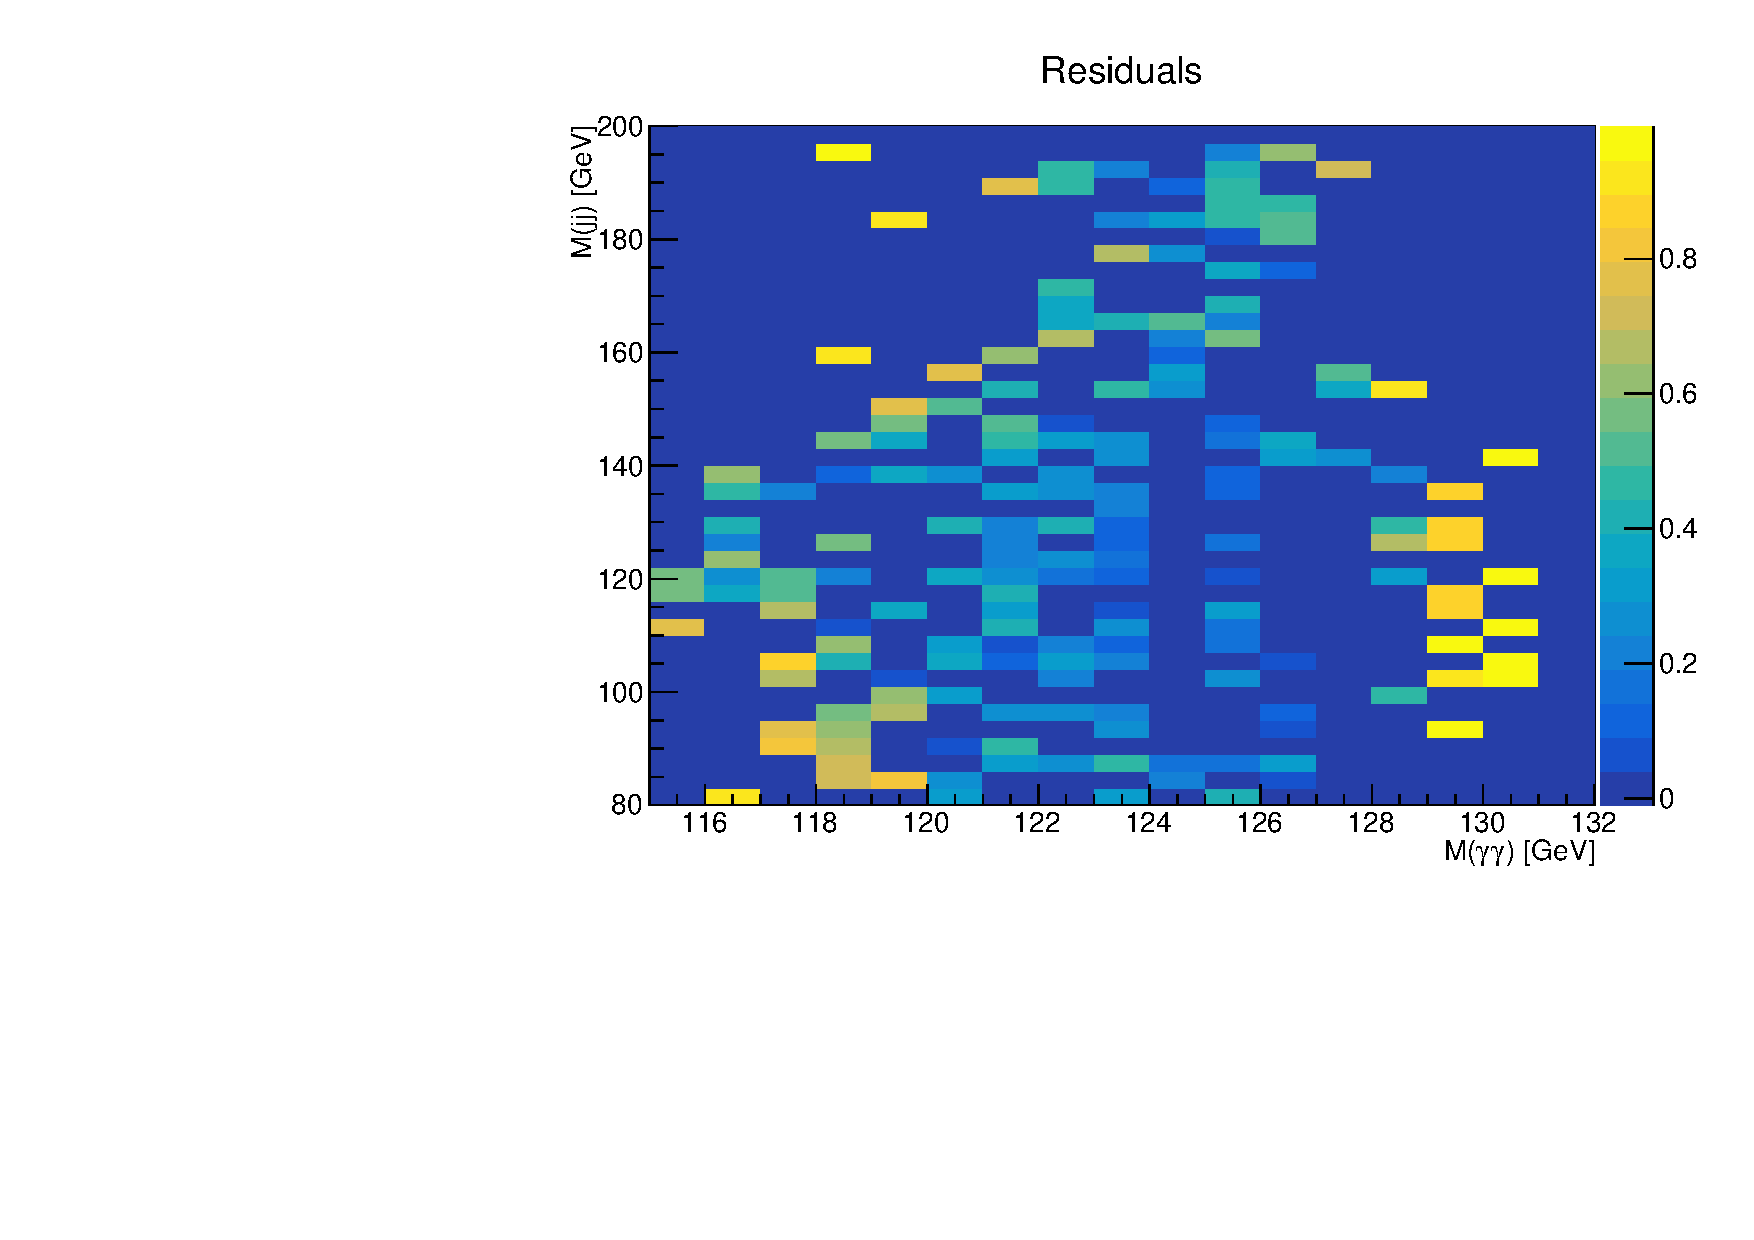
\includegraphics[width=0.3\textwidth]{figures/sec-signals/SignalResiduals/h_re_HM_cat0}\hfil
  \caption{2D distributions of the signal MC (left), fitted PDF model (center) and 2D residuals (right) for the High Mass-High Purity Category non-resonant selection.}
  \label{fig:sig_resi_hm_hpc}
\end{figure*}

\begin{figure*}[h]
  \centering
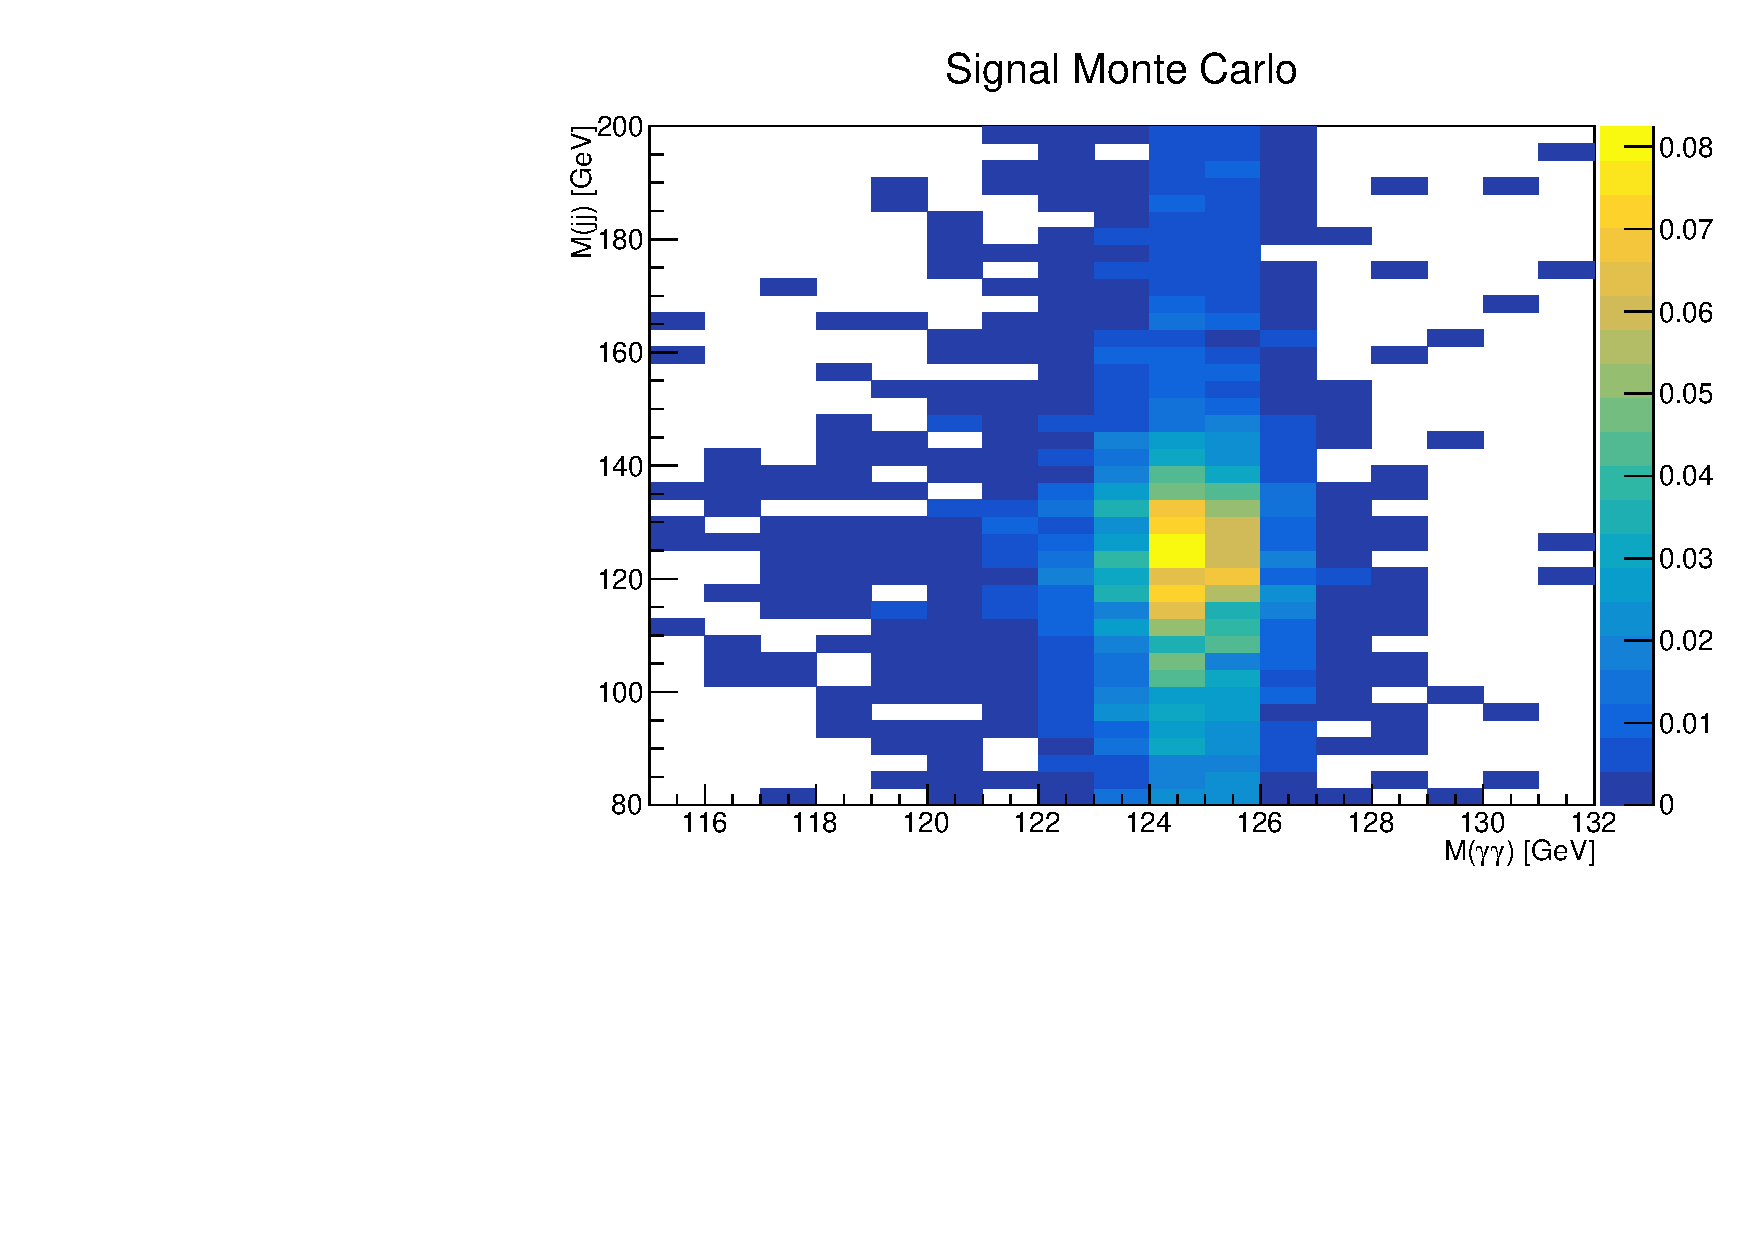
\includegraphics[width=0.3\textwidth]{figures/sec-signals/SignalResiduals/h_mc_HM_cat1}\hfil
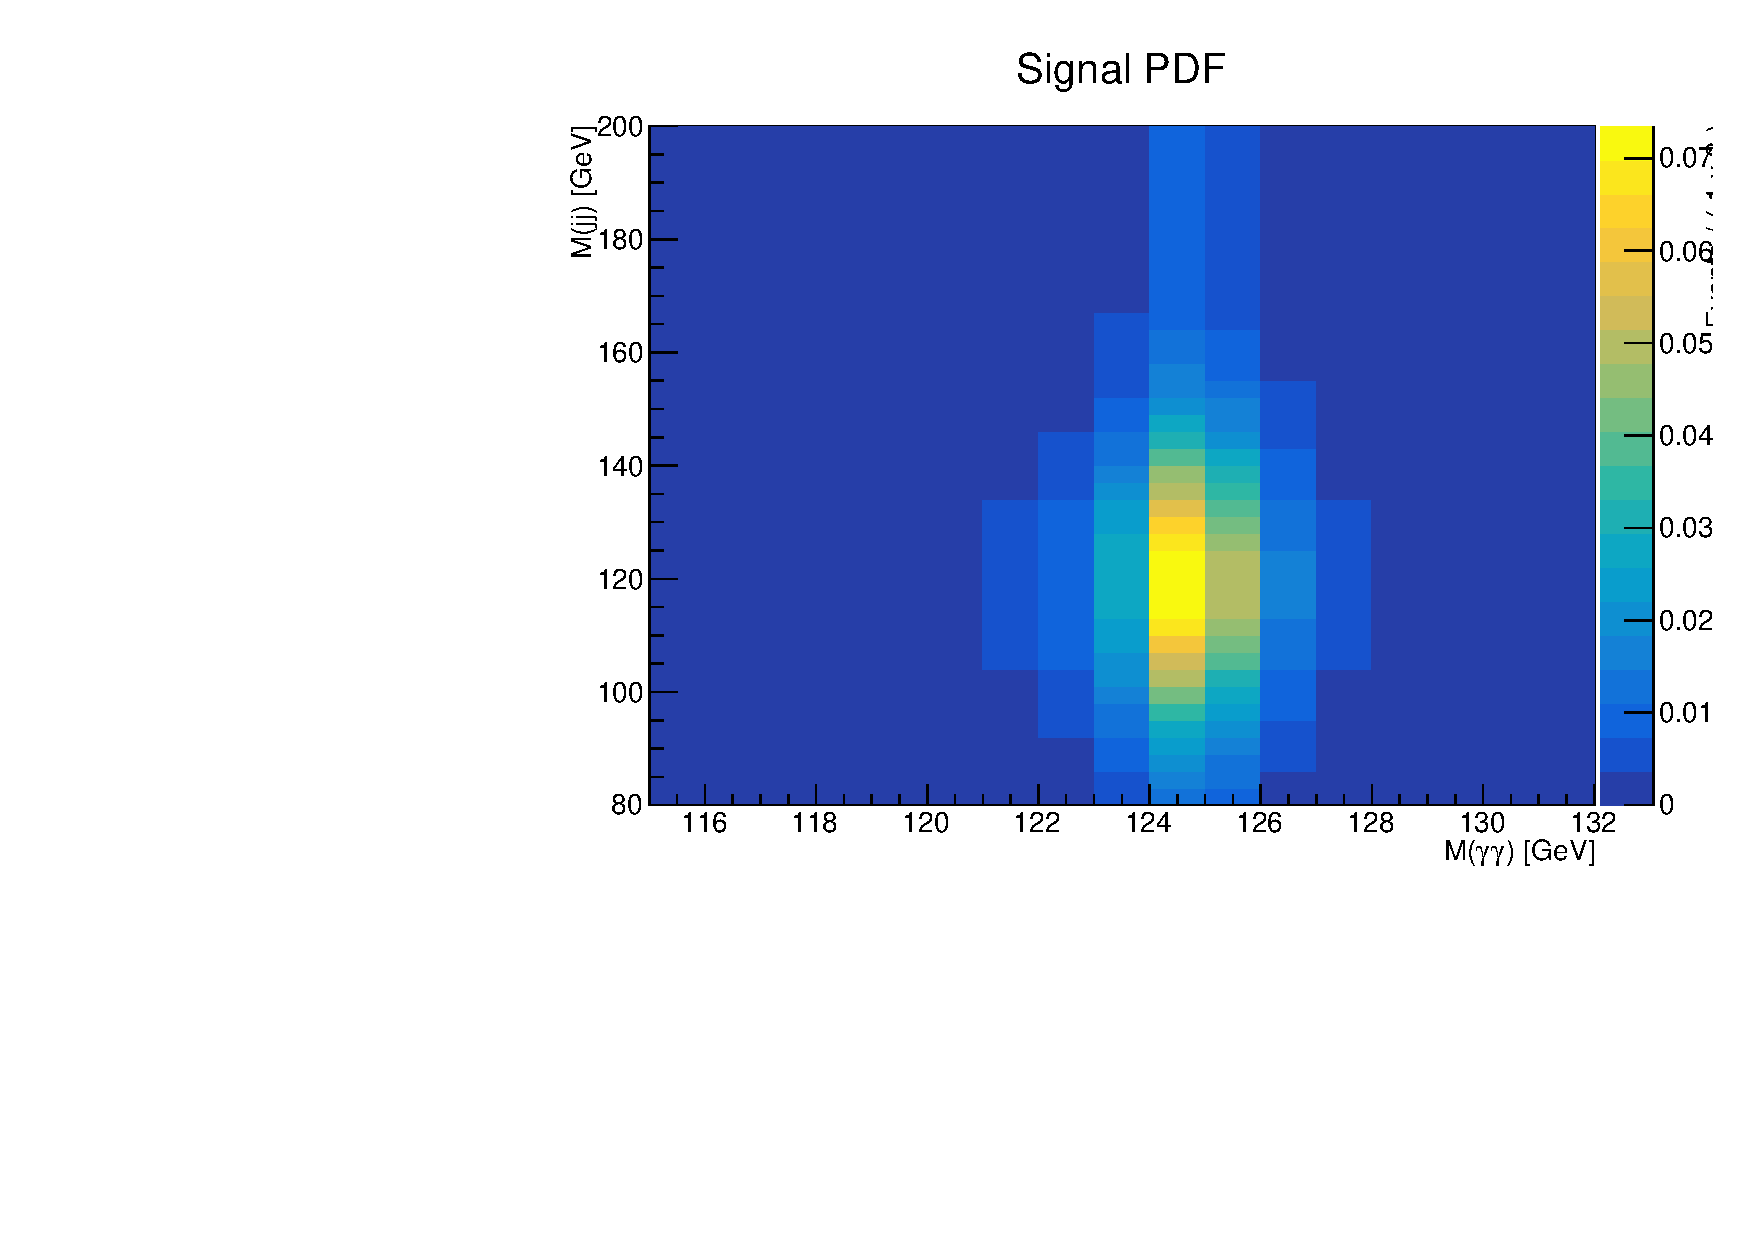
\includegraphics[width=0.3\textwidth]{figures/sec-signals/SignalResiduals/h_pd_HM_cat1}\hfil
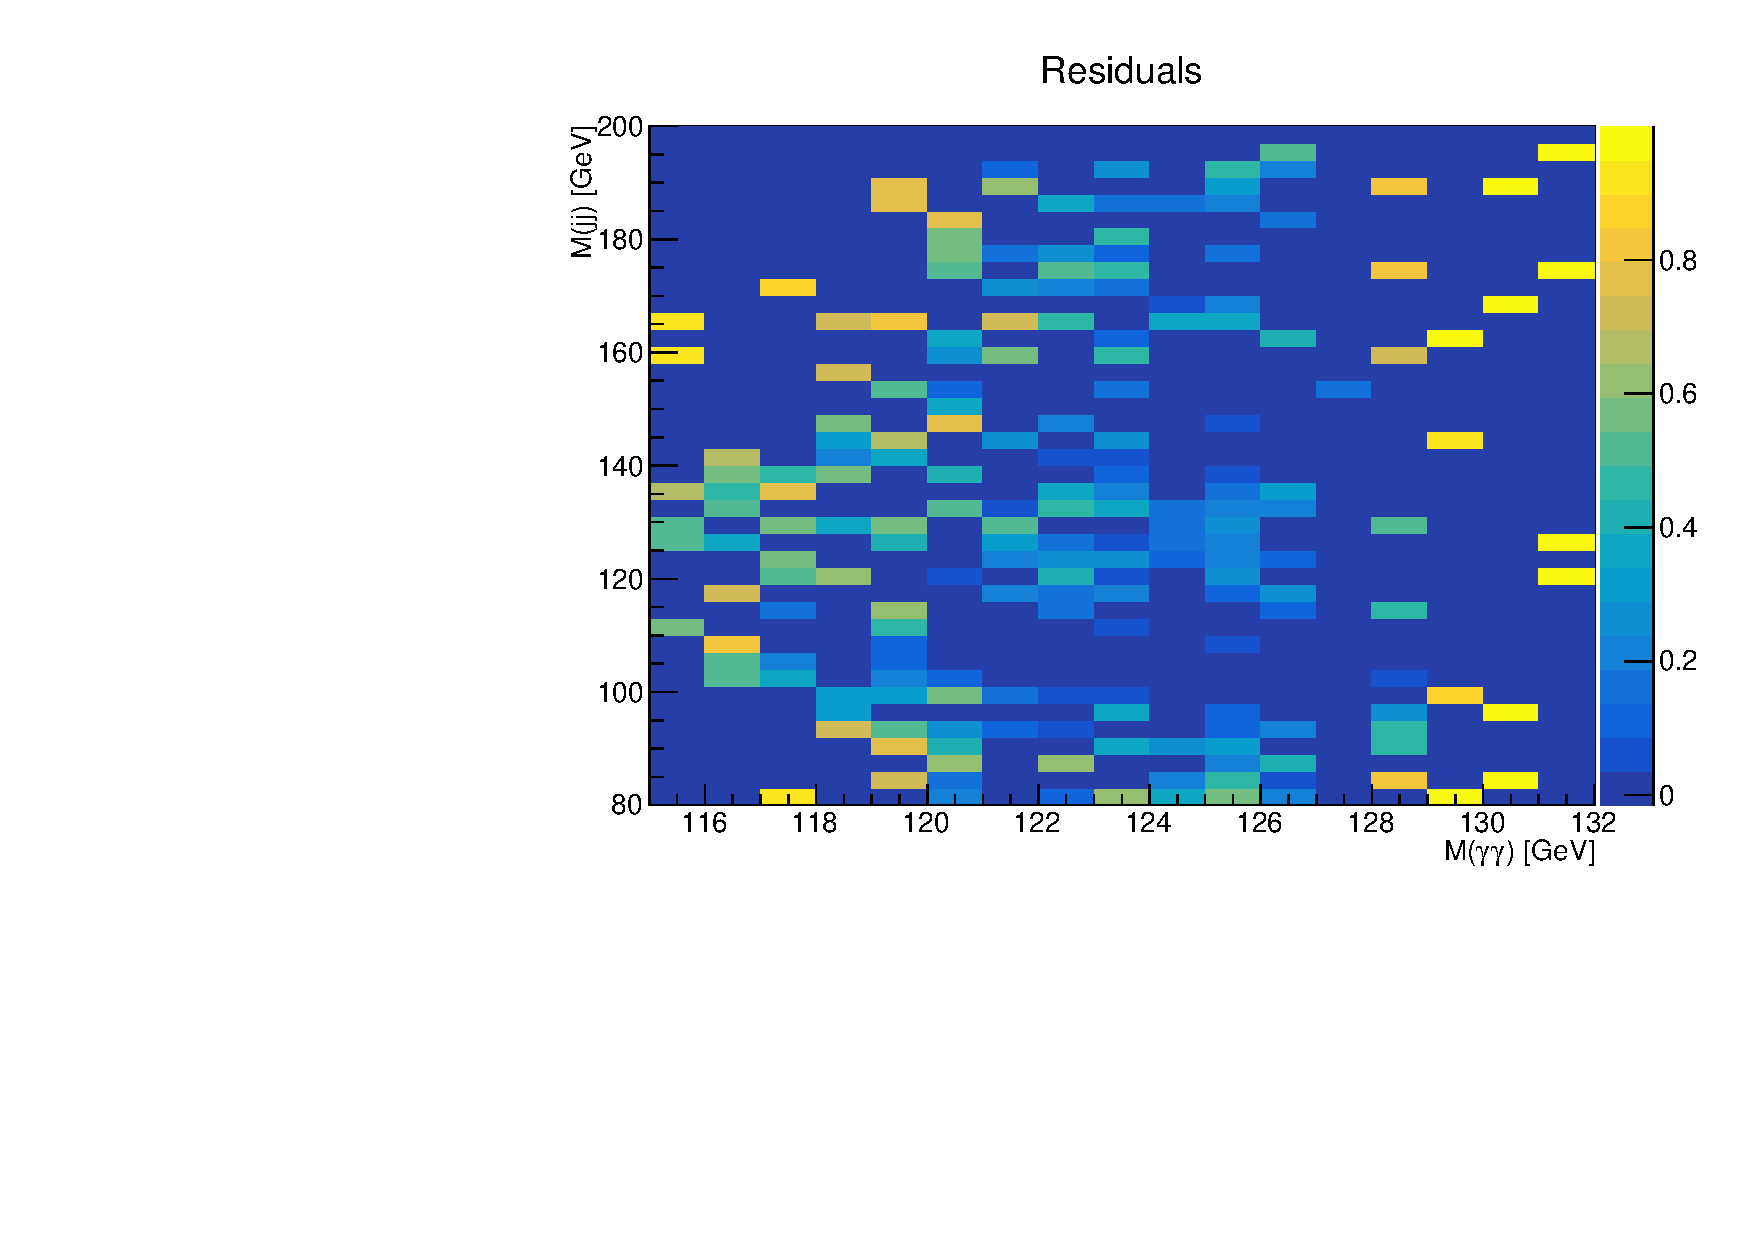
\includegraphics[width=0.3\textwidth]{figures/sec-signals/SignalResiduals/h_re_HM_cat1}\hfil
  \caption{2D distributions of the signal MC (left), fitted PDF model (center) and 2D residuals (right) for the High Mass-Medium Purity Category non-resonant selection.}
  \label{fig:sig_resi_hm_mpc}
\end{figure*}

\begin{figure*}[h]
  \centering
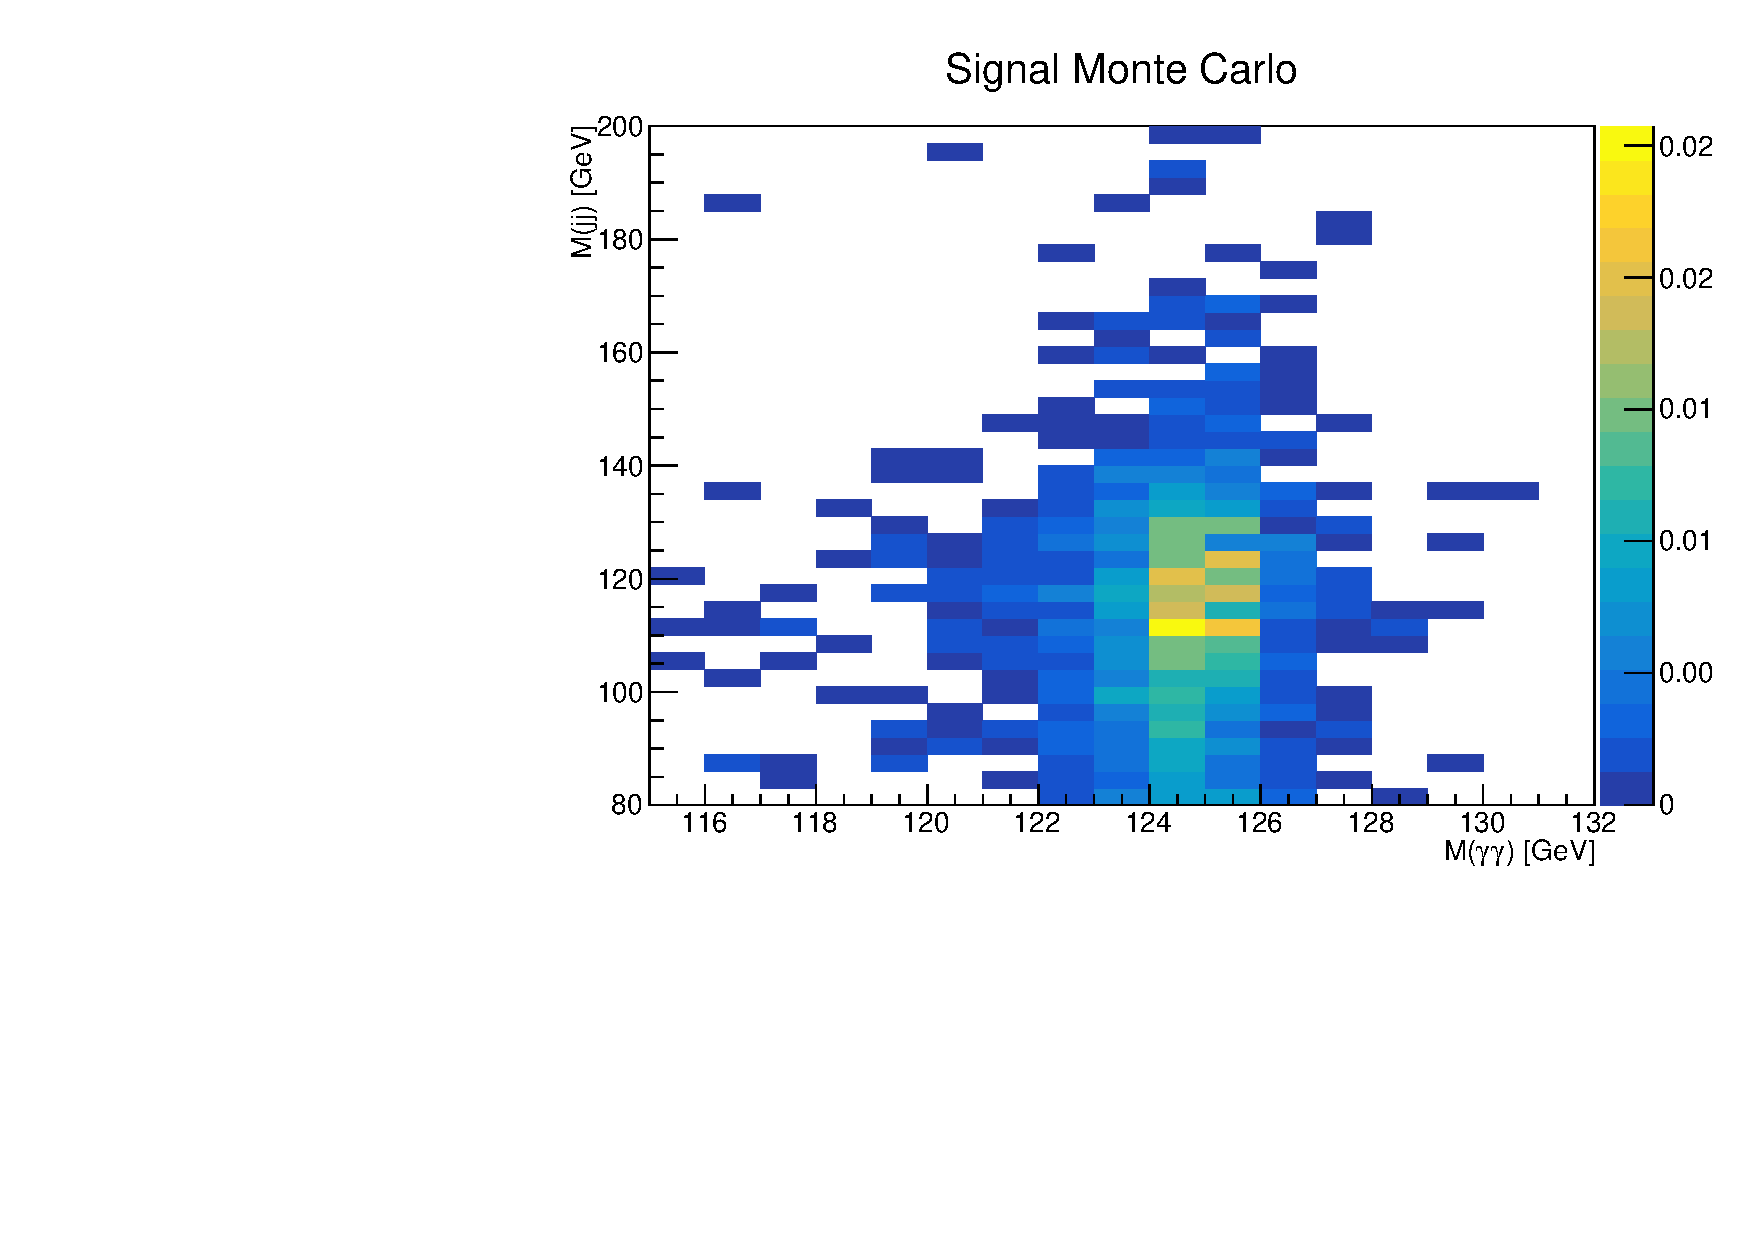
\includegraphics[width=0.3\textwidth]{figures/sec-signals/SignalResiduals/h_mc_LM_cat0}\hfil
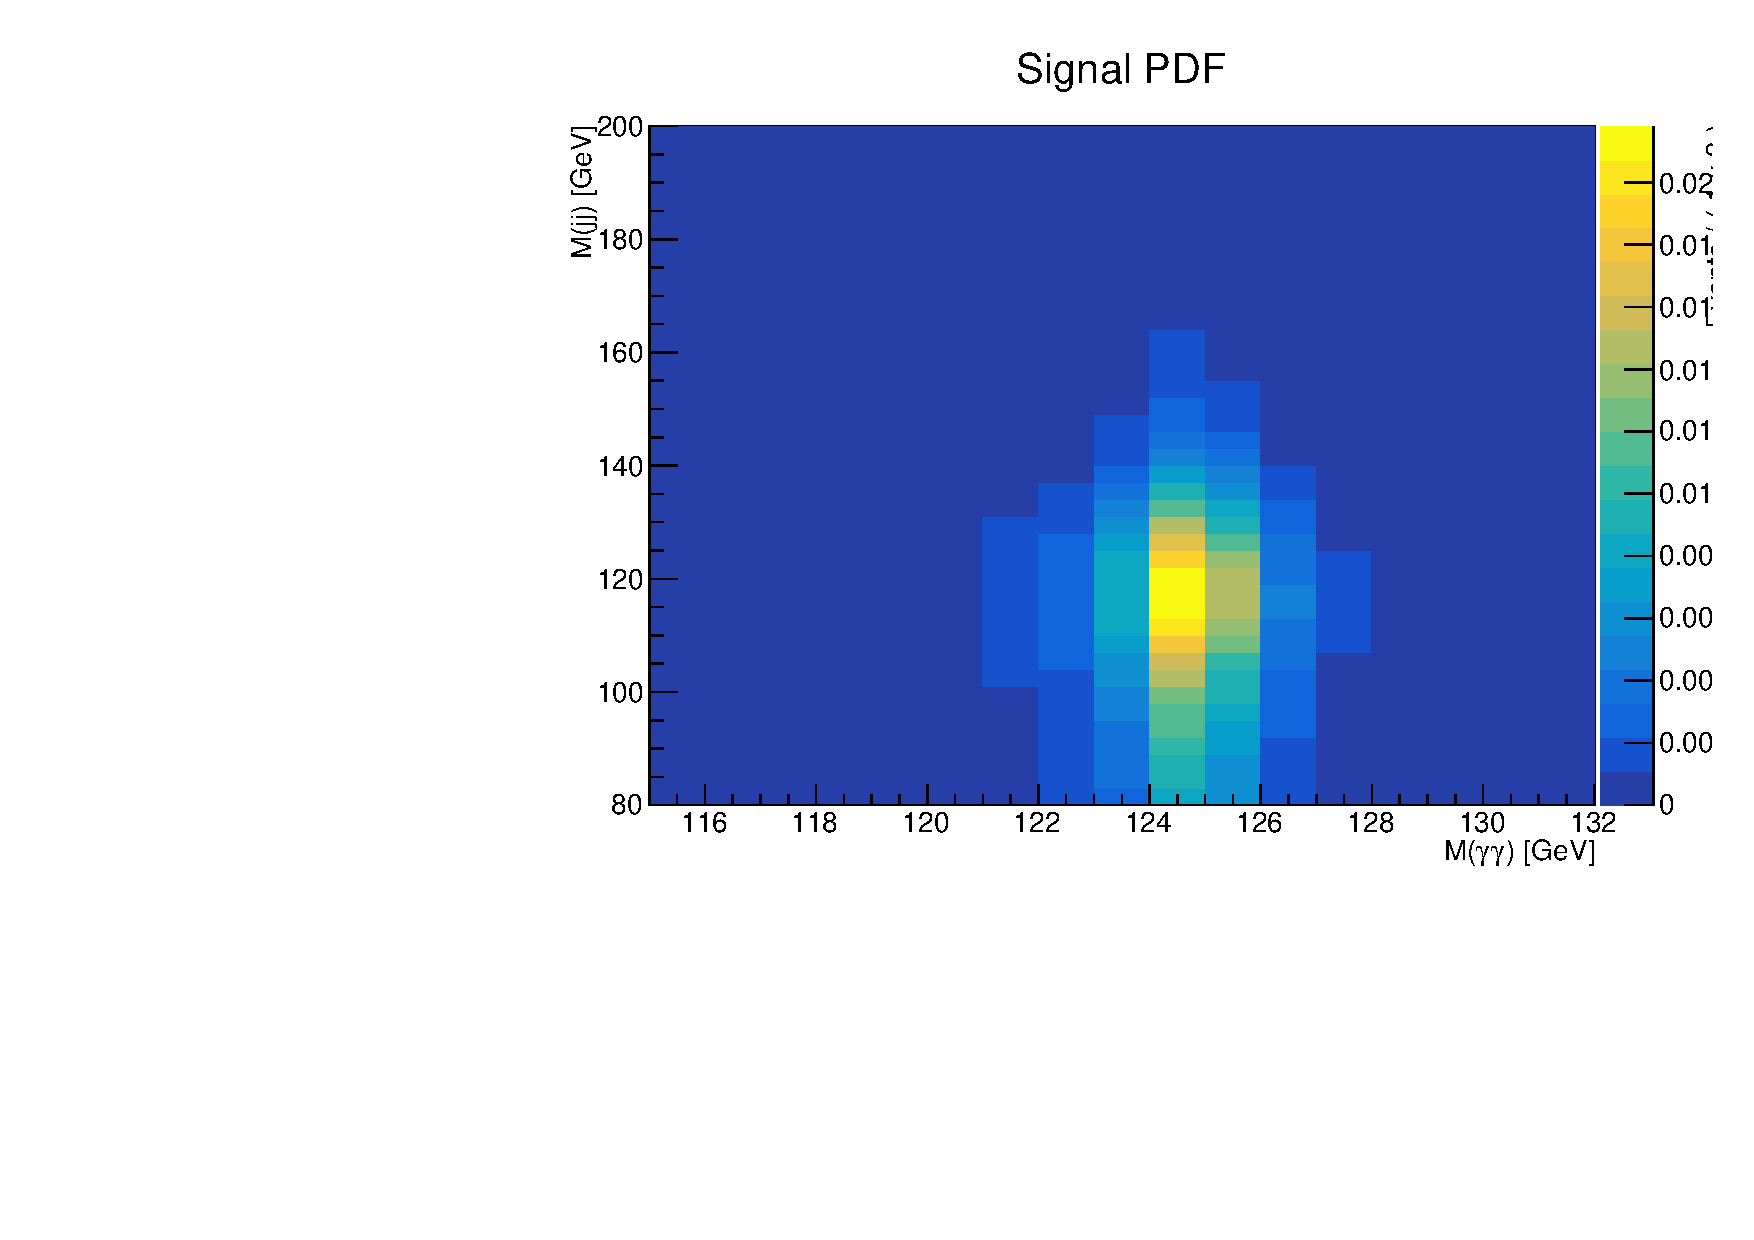
\includegraphics[width=0.3\textwidth]{figures/sec-signals/SignalResiduals/h_pd_LM_cat0}\hfil
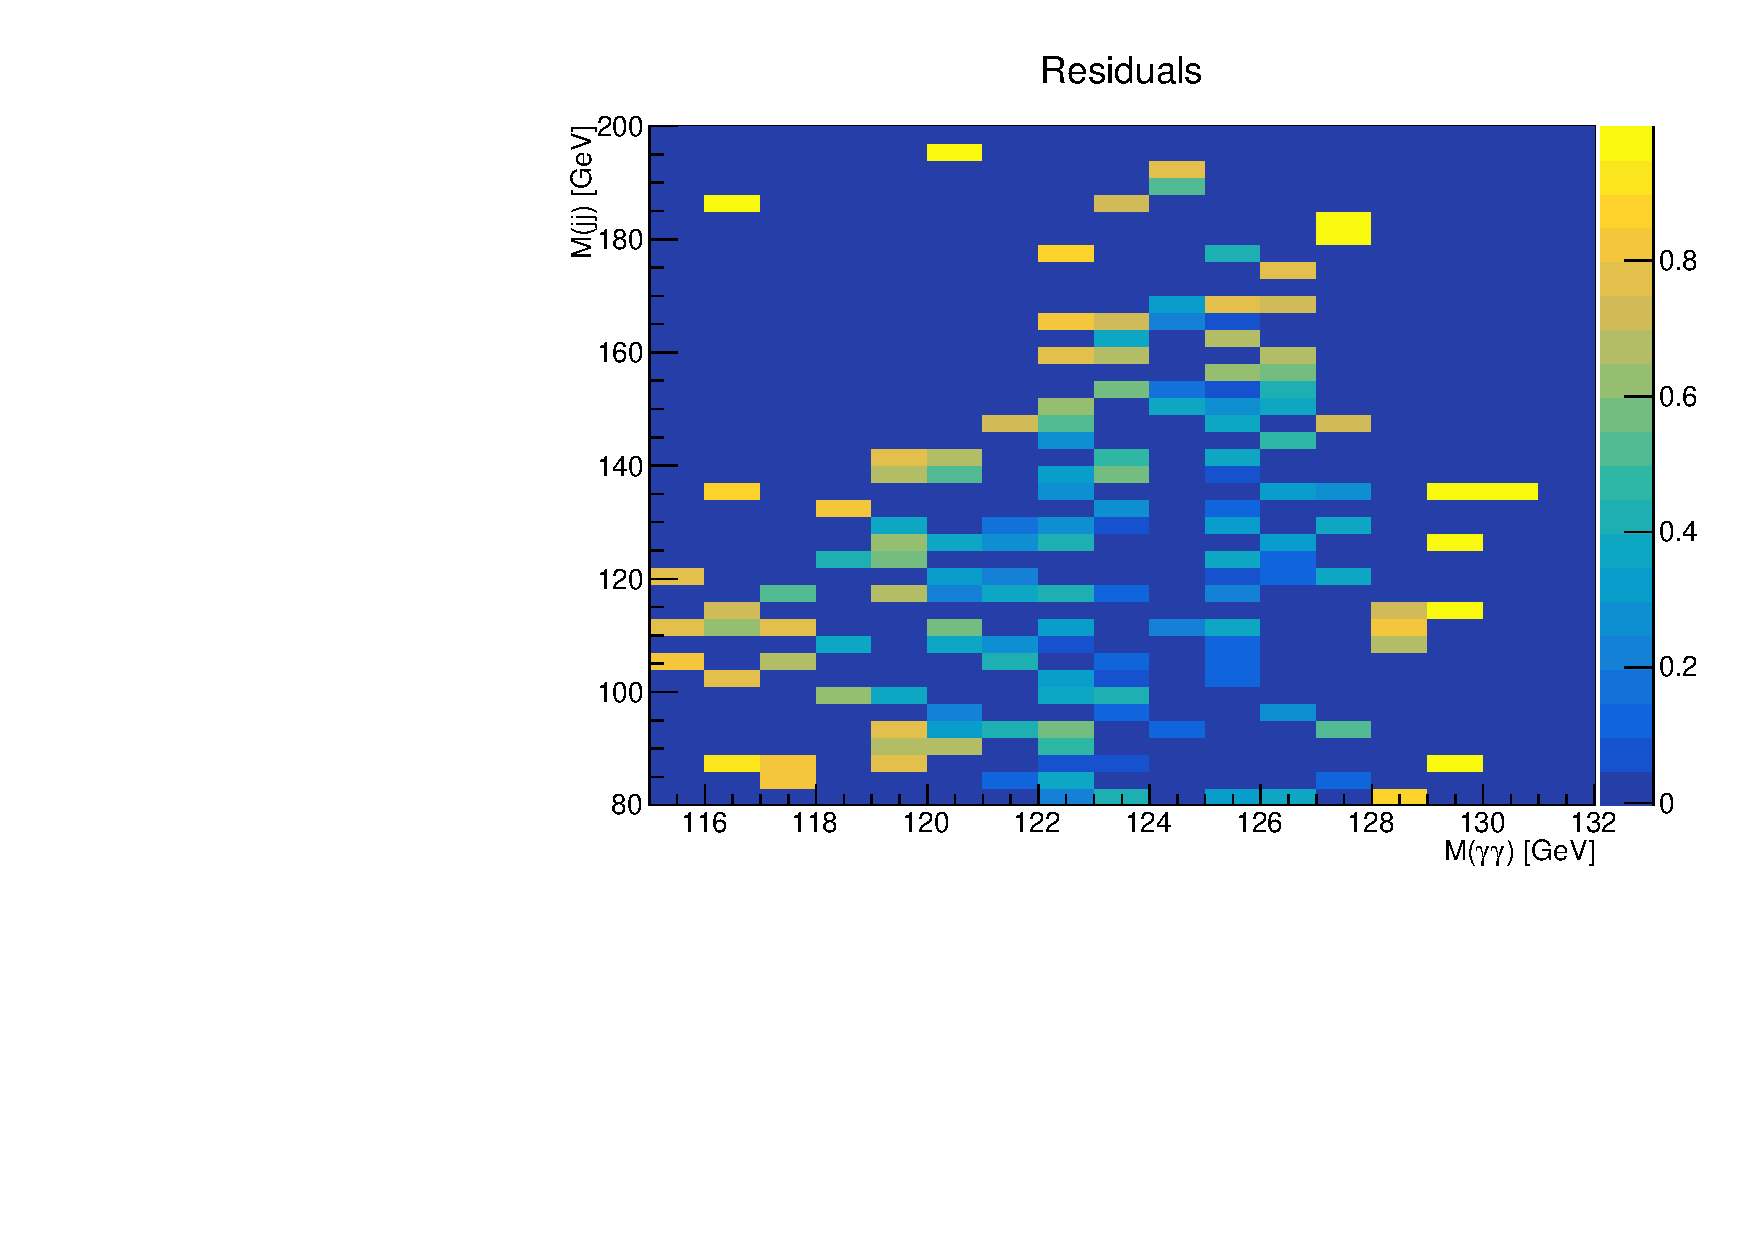
\includegraphics[width=0.3\textwidth]{figures/sec-signals/SignalResiduals/h_re_LM_cat0}\hfil
  \caption{2D distributions of the signal MC (left), fitted PDF model (center) and 2D residuals (right) for the Low Mass-High Purity Category non-resonant selection.}
  \label{fig:sig_resi_lm_hpc}
\end{figure*}


\begin{figure*}[h]
  \centering
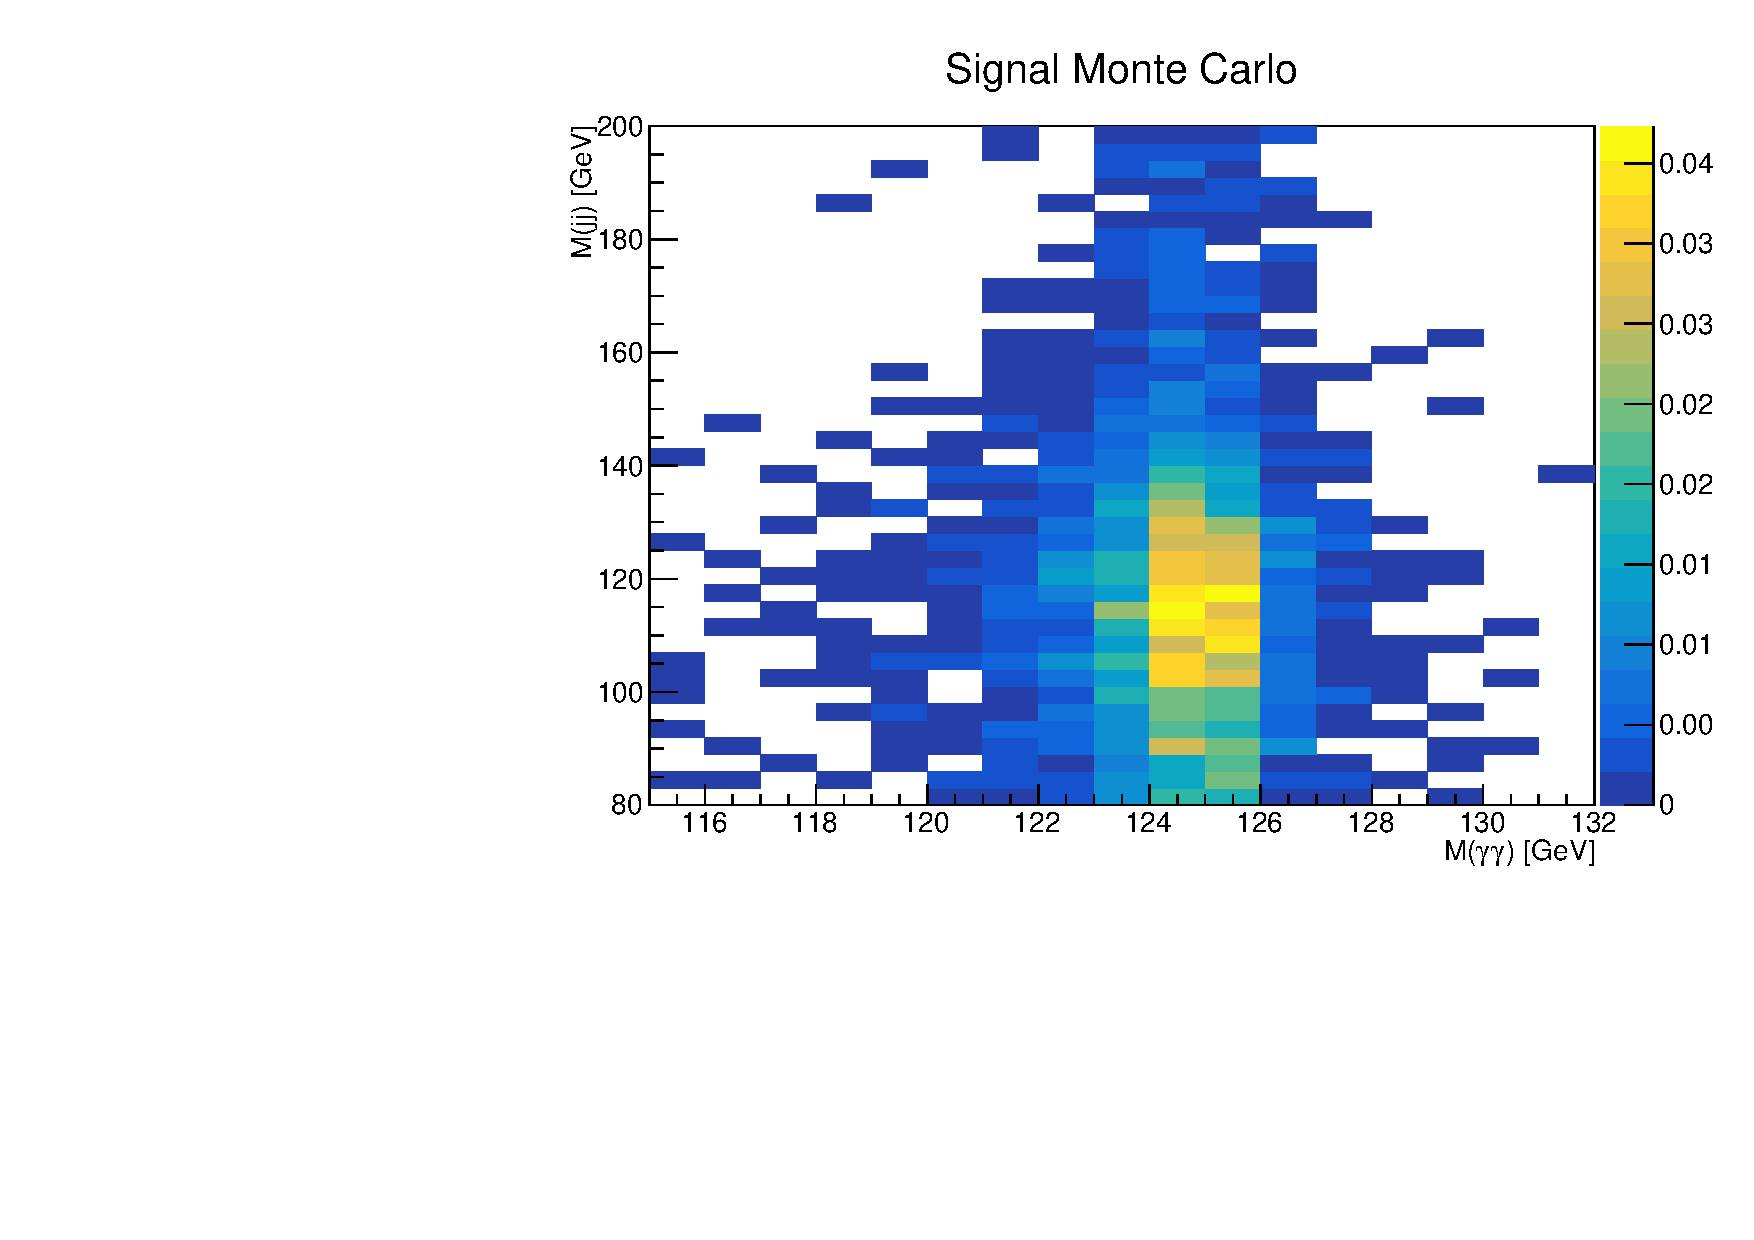
\includegraphics[width=0.3\textwidth]{figures/sec-signals/SignalResiduals/h_mc_LM_cat1}\hfil
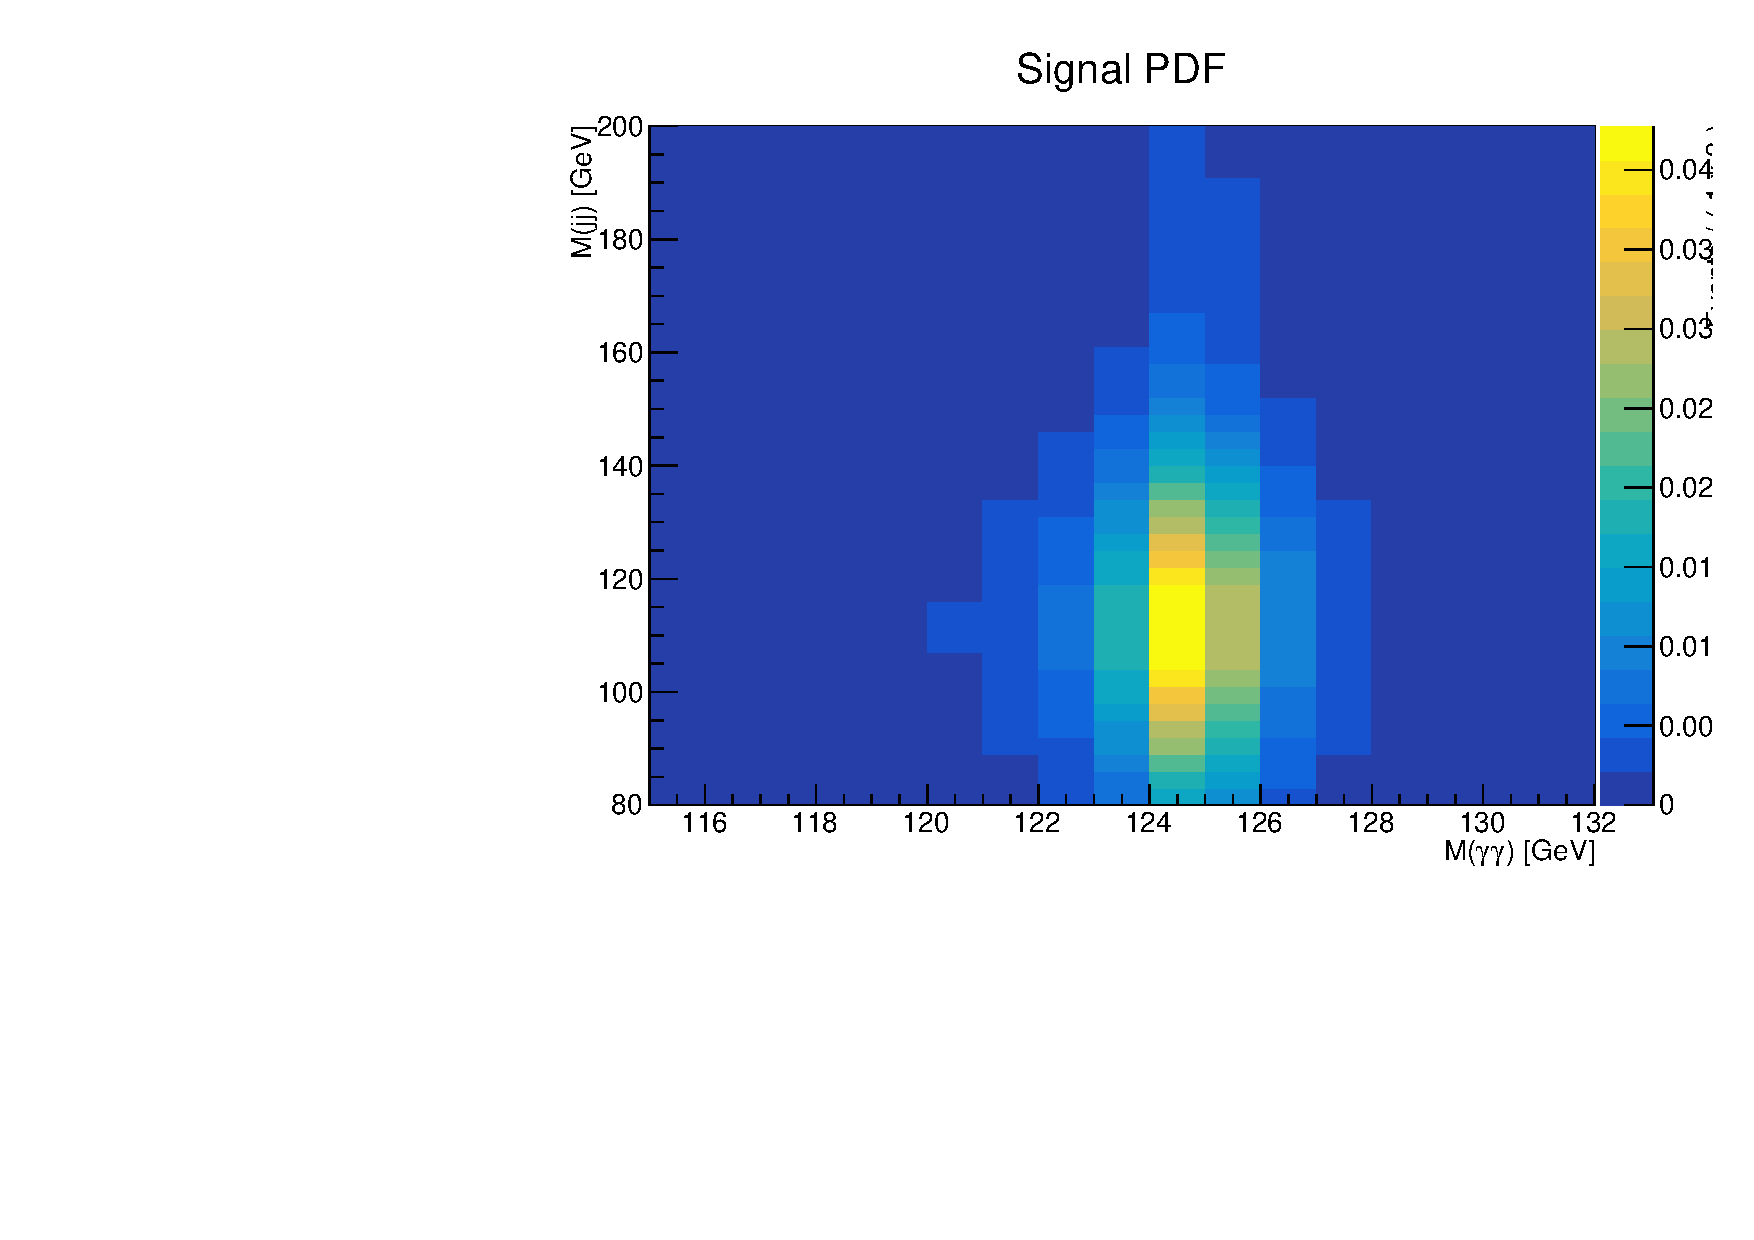
\includegraphics[width=0.3\textwidth]{figures/sec-signals/SignalResiduals/h_pd_LM_cat1}\hfil
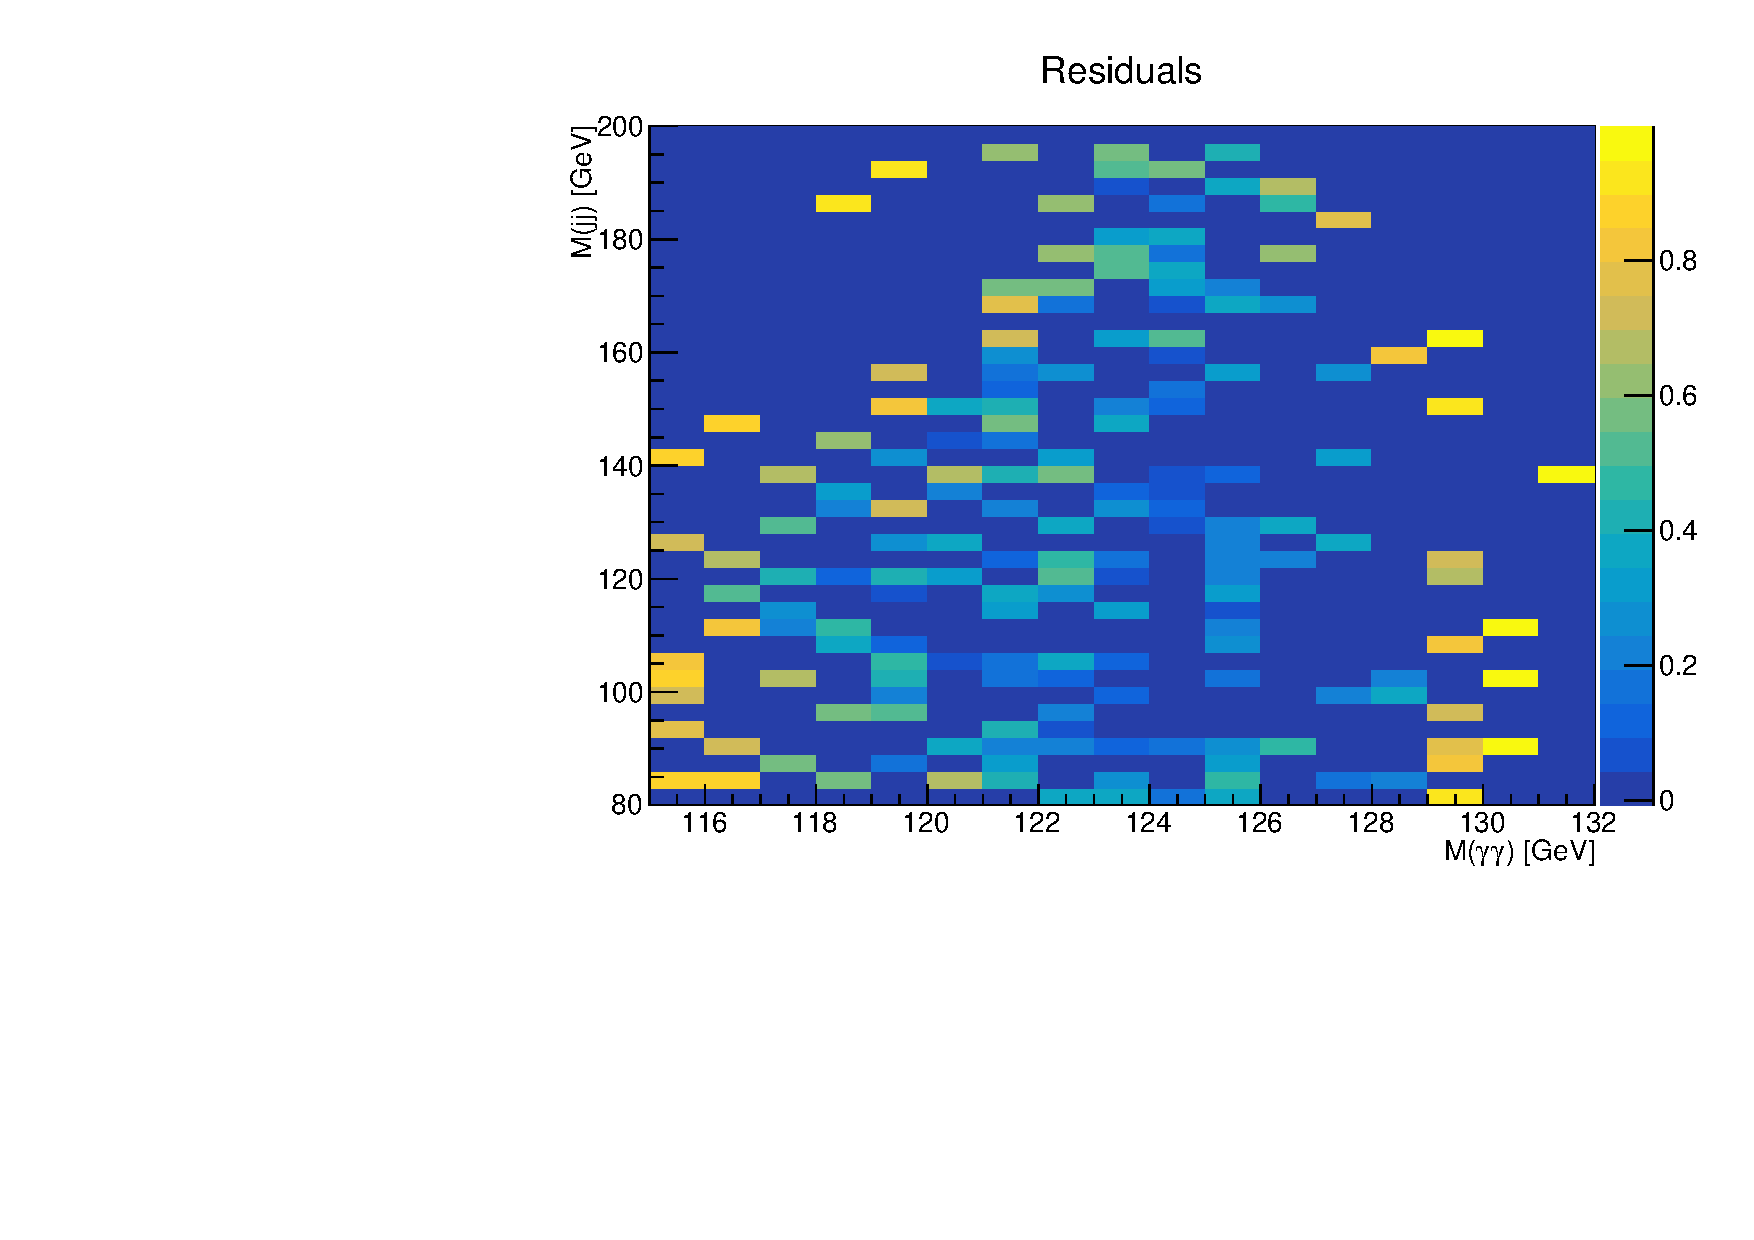
\includegraphics[width=0.3\textwidth]{figures/sec-signals/SignalResiduals/h_re_LM_cat1}\hfil
  \caption{2D distributions of the signal MC (left), fitted PDF model (center) and 2D residuals (right) for the Low Mass-Medium Purity Category non-resonant selection.}
  \label{fig:sig_resi_lm_mpc}
\end{figure*}



\subsection{Background Model}

To study the background fits, we use the fake photon control region (one photon in the diphoton candidate fails the identification requirements). From this control region, we randomly pick the number of events that is expected from the signal region under study according to the control sample described in section \label{sec:PCR}.

The functional choice to model the background in both fitting variables is the Bernstein family of polynomials. 
We also assume that the same order of polynomial is to be used in both variables. 
This comes from the fact that the order of the polynomial is related to the precision of the fit (degrees of freedom), which, in turn, is related to the number of events being fitted. 

%To estimate the background in $\Mgg$ and $\Mjj$, we use three families of functions as possible fits: Bernstein polynomials, Power Laws and Exponentials. The Bernstein polynomials are used instead of standard ones because their coefficients are positive definite, making the minimization process in the fitting more stable.

The first study performed is the order fixing. 
We fit consecutive orders of the three families of functions and check the difference between the negative log-likelihoods times two ($2\Delta NLL$) between the two consecutive fits. 
This $2\Delta NLL$ should be distributed as a $\chi^{2}(\alpha)$ distribution with the number of degrees of freedom equal to the difference in number of free parameters between the two consecutive orders ($\alpha$). 
We then calculate the p-value of having a $2\Delta NLL$ higher than the one calculated before, given the $\chi^{2}(\alpha)$ distribution. 
If this p-value is lower than 0.05, we accept the higher order function, and continue the procedure for the next order. 
If this p-value is higher than 0.05, the higher order function is assumed to be too flexible given the data and the procedure terminates having found the lowest order suitable function.

Due to the different regimes of our signal regions after the mass window requirements and of the non-resonant selection, it is expected that our fits will involve very different background yields. 
For that, we perform the $2\Delta NLL$ test in all different signal regions. 
The results of this test are regions of validity in number of background events to be fit. 
This means that the choice of Bernstein order will depend on the number of events being fitted in a given signal region. 
The results of the study show that, for fits with less than 15 events, a first order Benstein passes the $2\Delta NLL$ test. 
For fits with 25 or more events, but less than 200, a second order Bernstein passes the $2\Delta NLL$ test. 
For fits with 200 or more events, a third order Bernstein passes the $2\Delta NLL$ test. 

\subsubsection{Bias Studies}

After the order fixing, we must ensure that the functional form chosen does not bias a possible signal strength measurement in the analysis. This can happen because the real background shape that is being fitted might not be exactly the chosen functional form. Since we have no way of defining what this true shape is, we compare the signal strength measured ($\mu$) from the background models with respect to different background shape hypotheses, as produced by a toy Monte Carlo.

The goal is to find at least one background model that can fit other background shapes without a statistically significant bias in the signal strength reconstruction. The goal of having a background model with a bias less than 0.14 for all assumed shapes is set. This is justified by investigating the effect that a signal strength bias can be correct by increasing the uncertainty on $\mu$ until the true value is within the $1\sigma$ coverage of $\mu$. 

We compare our 2D Bernstein model to models constructed with a Laurent series for both $\Mgg$ and $\Mjj$, and with sums of exponentials for both $\Mgg$ and $\Mjj$. 
We construct models with different Laurent and exponential sum orders. 

The first step in the bias studies is to get pre-fit shapes of all background models. 
This is done in the same datasets used for the order fixing procedure: fake photon control region scaled to match the statistics found in different data signal regions. 

After the pre-fit shapes are constructed, toy Monte Carlo events are generated based on the pre-fitted background models. 2000 toy datasets are thrown for each background model. These toys are thrown injecting also signal events, according to the signal yields expected in each category. For that, we assume a signal cross section of 1 fb, for all resonant mass points and non-resonant benchmark points. Finally, the third step is fitting the 9 batches of toy datasets with the same background models and extracting the $\mu$ from each of the 2000 toy datasets. %Both the toy generation and the fitting steps are done with the CMS combine tool.

Some examples of the measured biases can be seen in Figures \ref{fig:bkg_bias1}-\ref{fig:bkg_bias4}. 
The x-axes on these plots represent a truth model with which toy MC was produced, while the y-axes represent the function used to fit the toy MC. 
The numbers on each bin are the absolute values of the biases on the signal strength measurements under a background hypothesis in the x-axis and a fit function in the y-axis. 

\begin{figure*}[h]
  \centering
  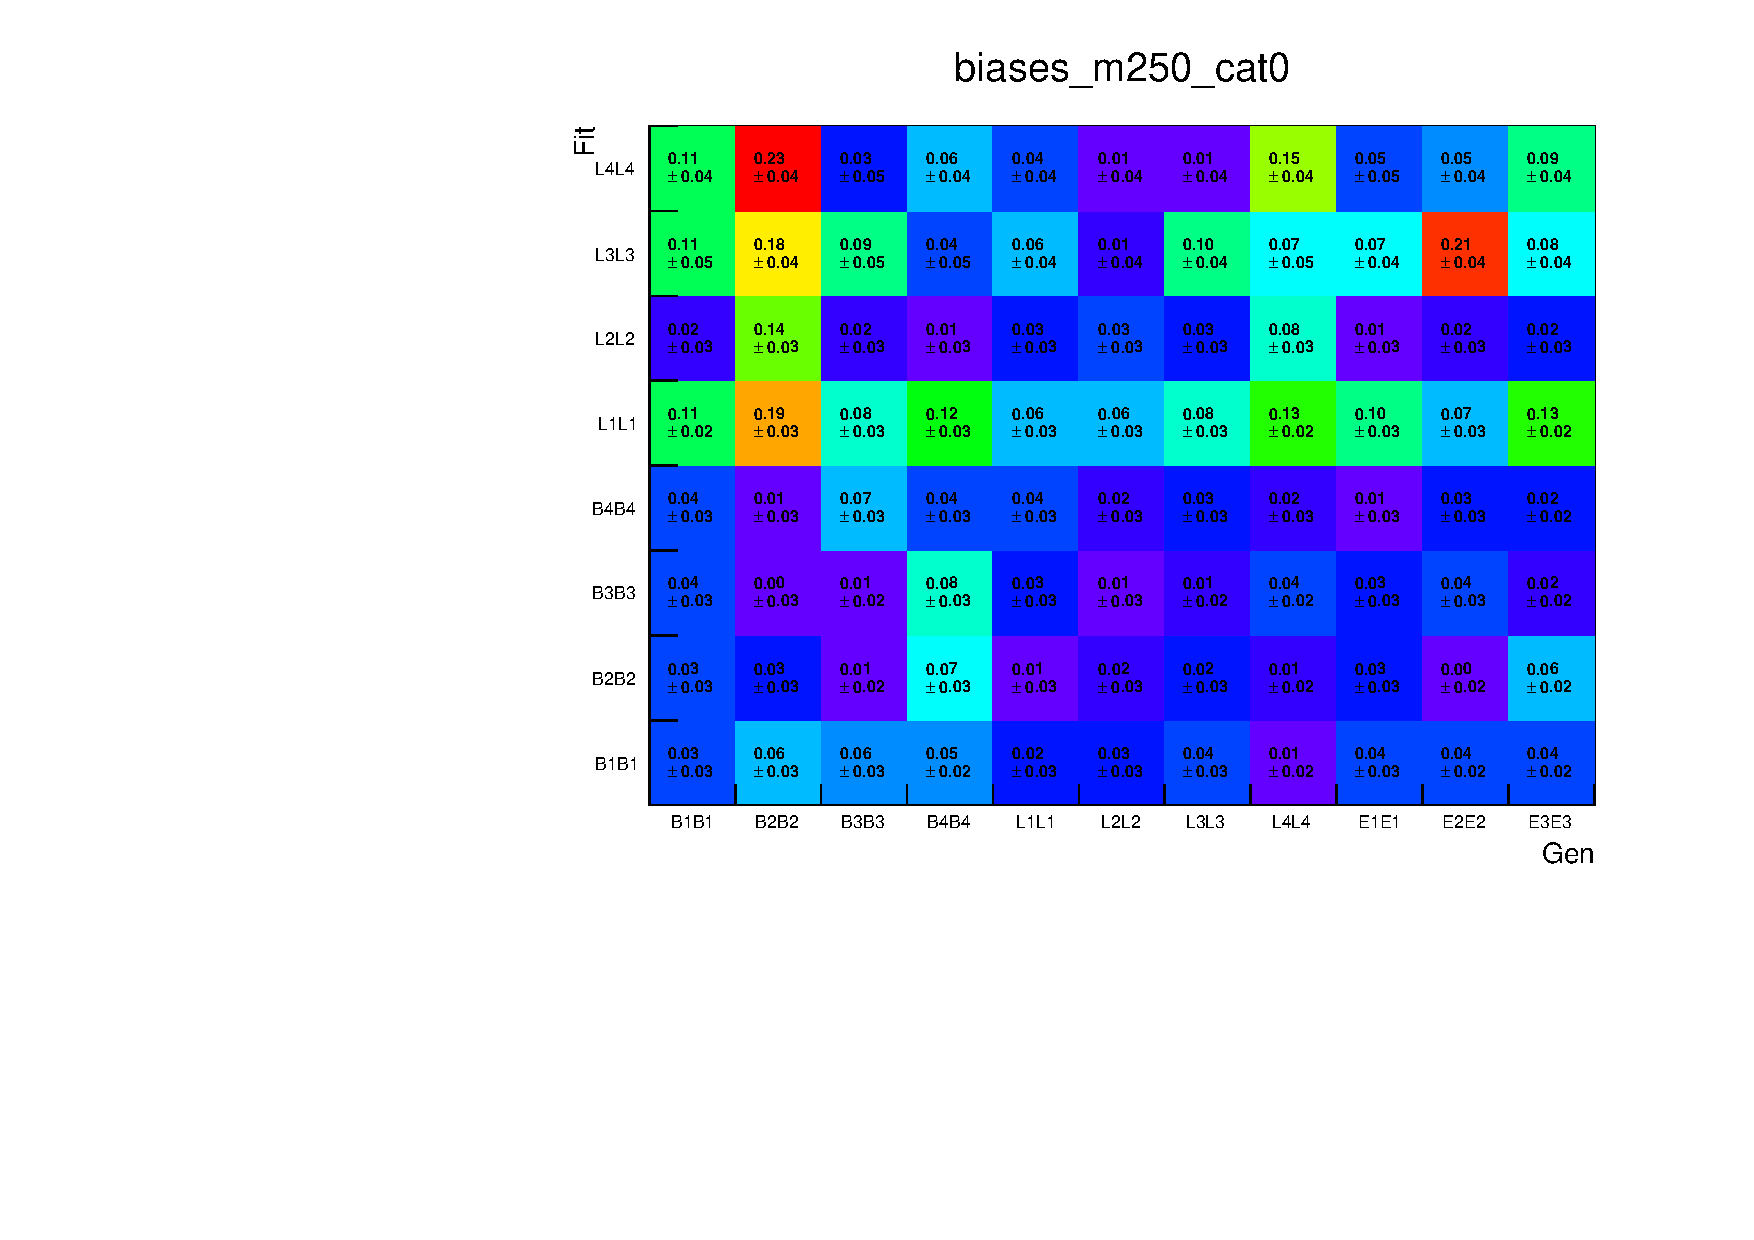
\includegraphics[width=0.48\textwidth]{figures/sec-bias/biases_m250_cat0.pdf}\hfil
  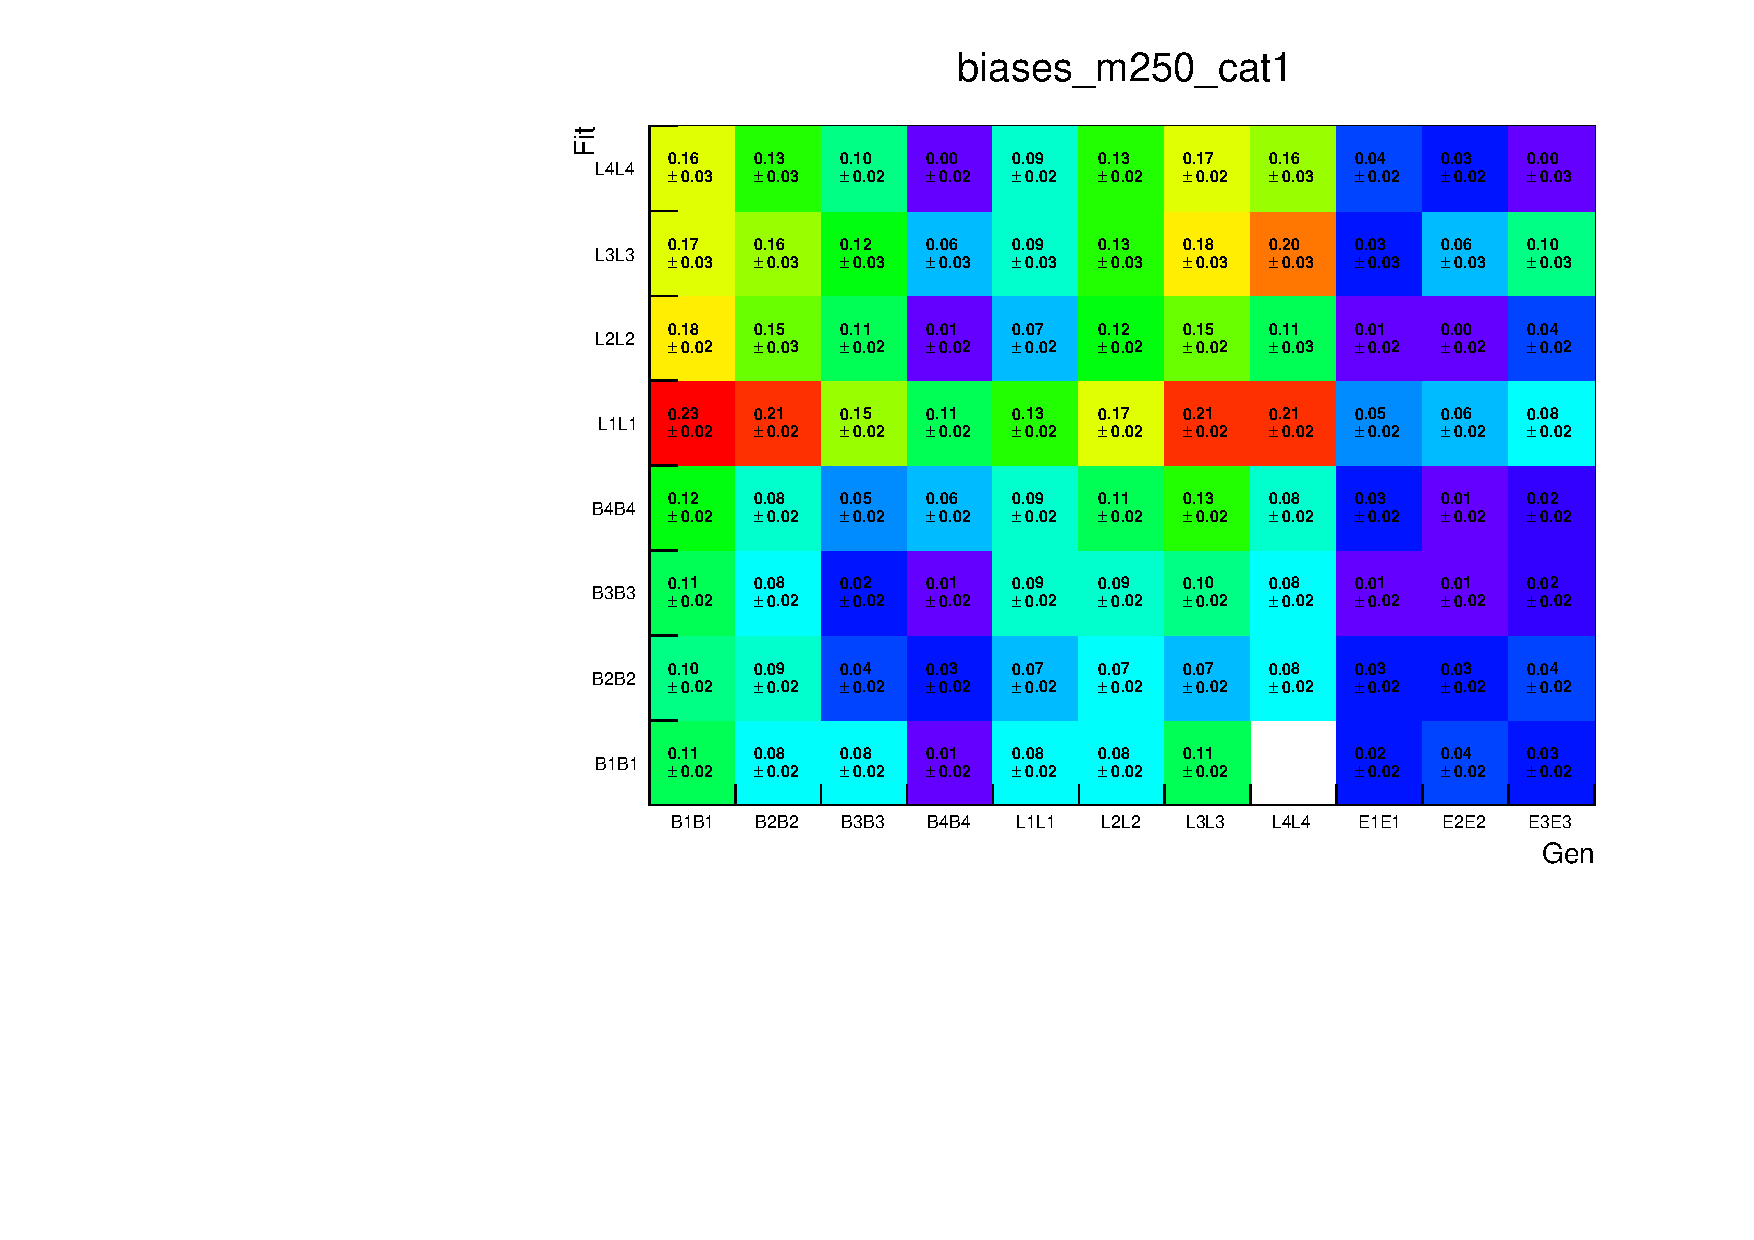
\includegraphics[width=0.48\textwidth]{figures/sec-bias/biases_m250_cat1.pdf}\hfil
  \caption{Biases measured in the 250 GeV resonant selection in the HPC (left) and MPC (right).}
  \label{fig:bkg_bias1}
\end{figure*}
\begin{figure*}[h]
  \centering
  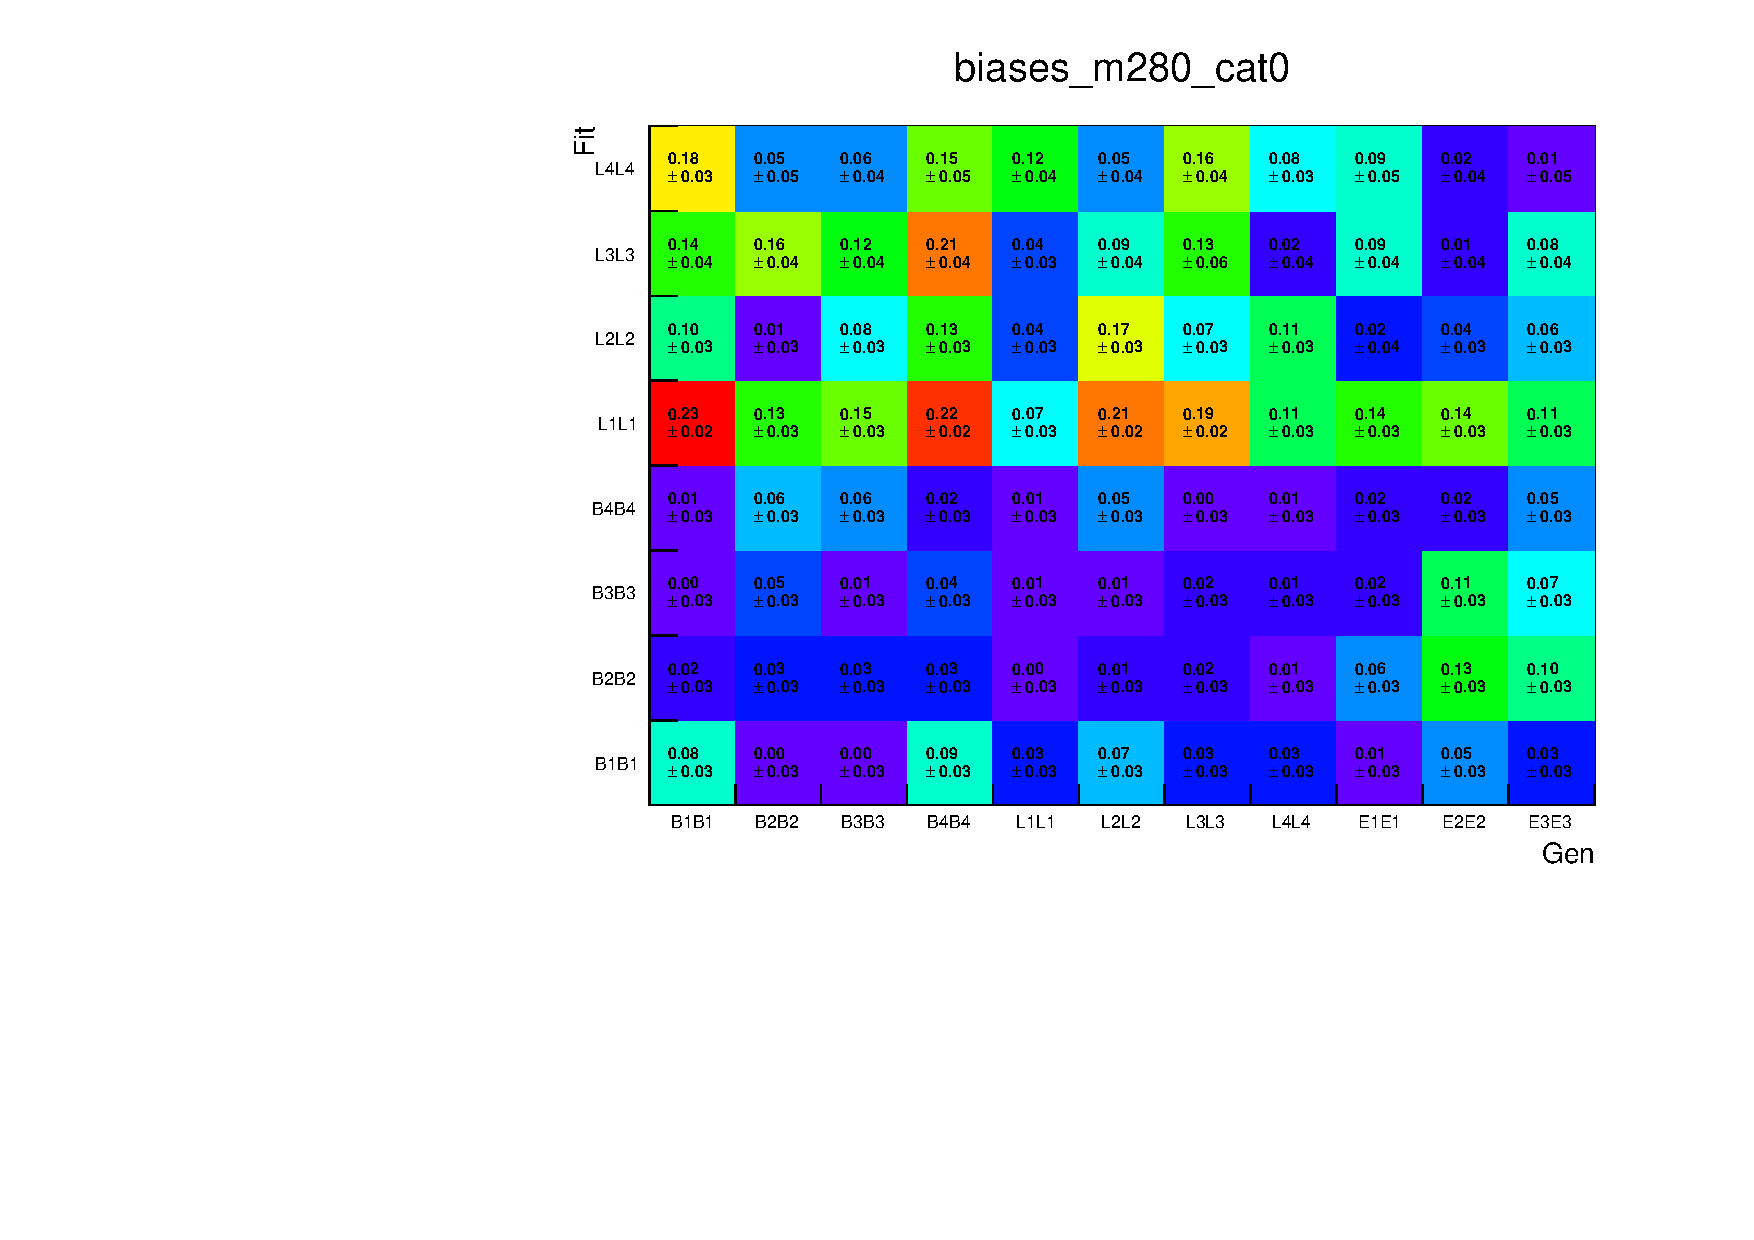
\includegraphics[width=0.48\textwidth]{figures/sec-bias/biases_m280_cat0.pdf}\hfil
  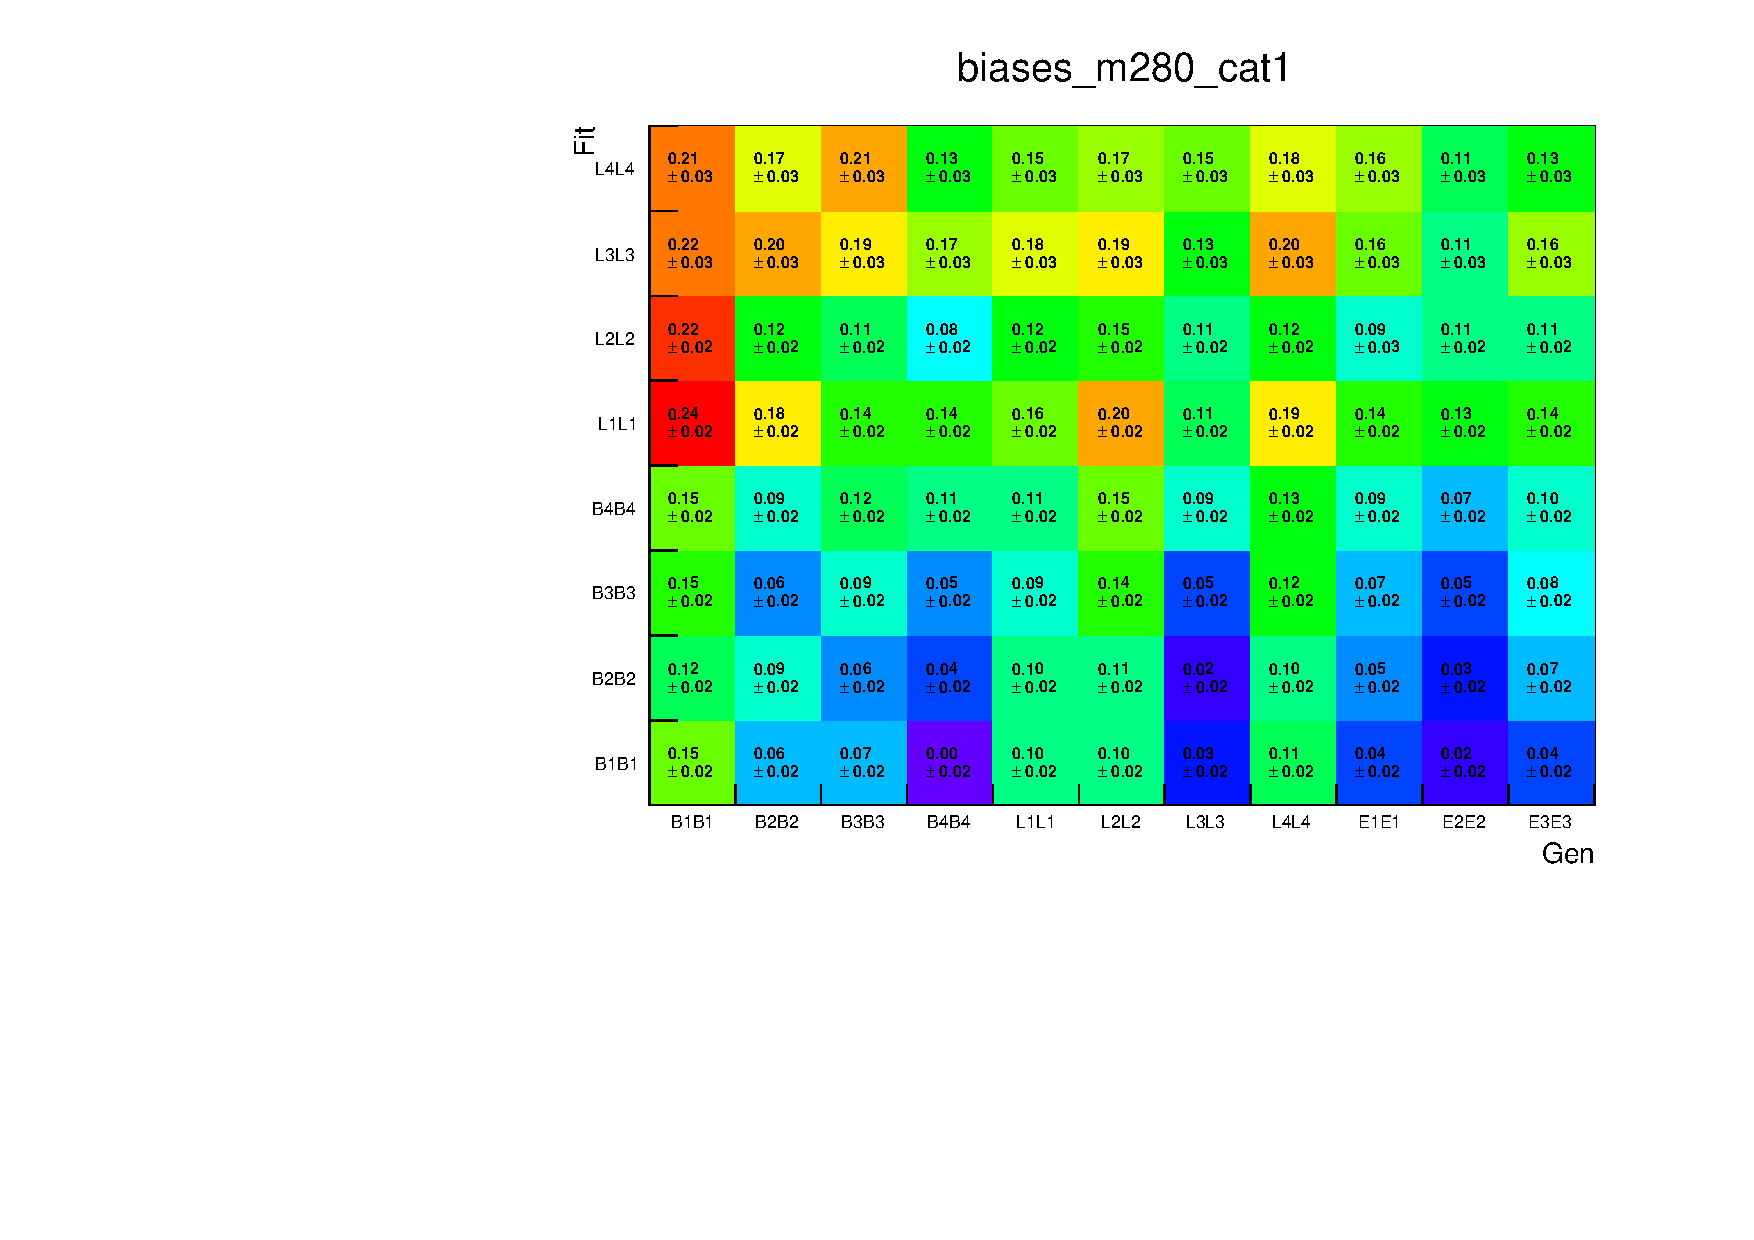
\includegraphics[width=0.48\textwidth]{figures/sec-bias/biases_m280_cat1.pdf}\hfil
  \caption{Biases measured in the 280 GeV resonant selection in the HPC (left) and MPC (right).}
  \label{fig:bkg_bias2}
\end{figure*}
\begin{figure*}[h]
  \centering
  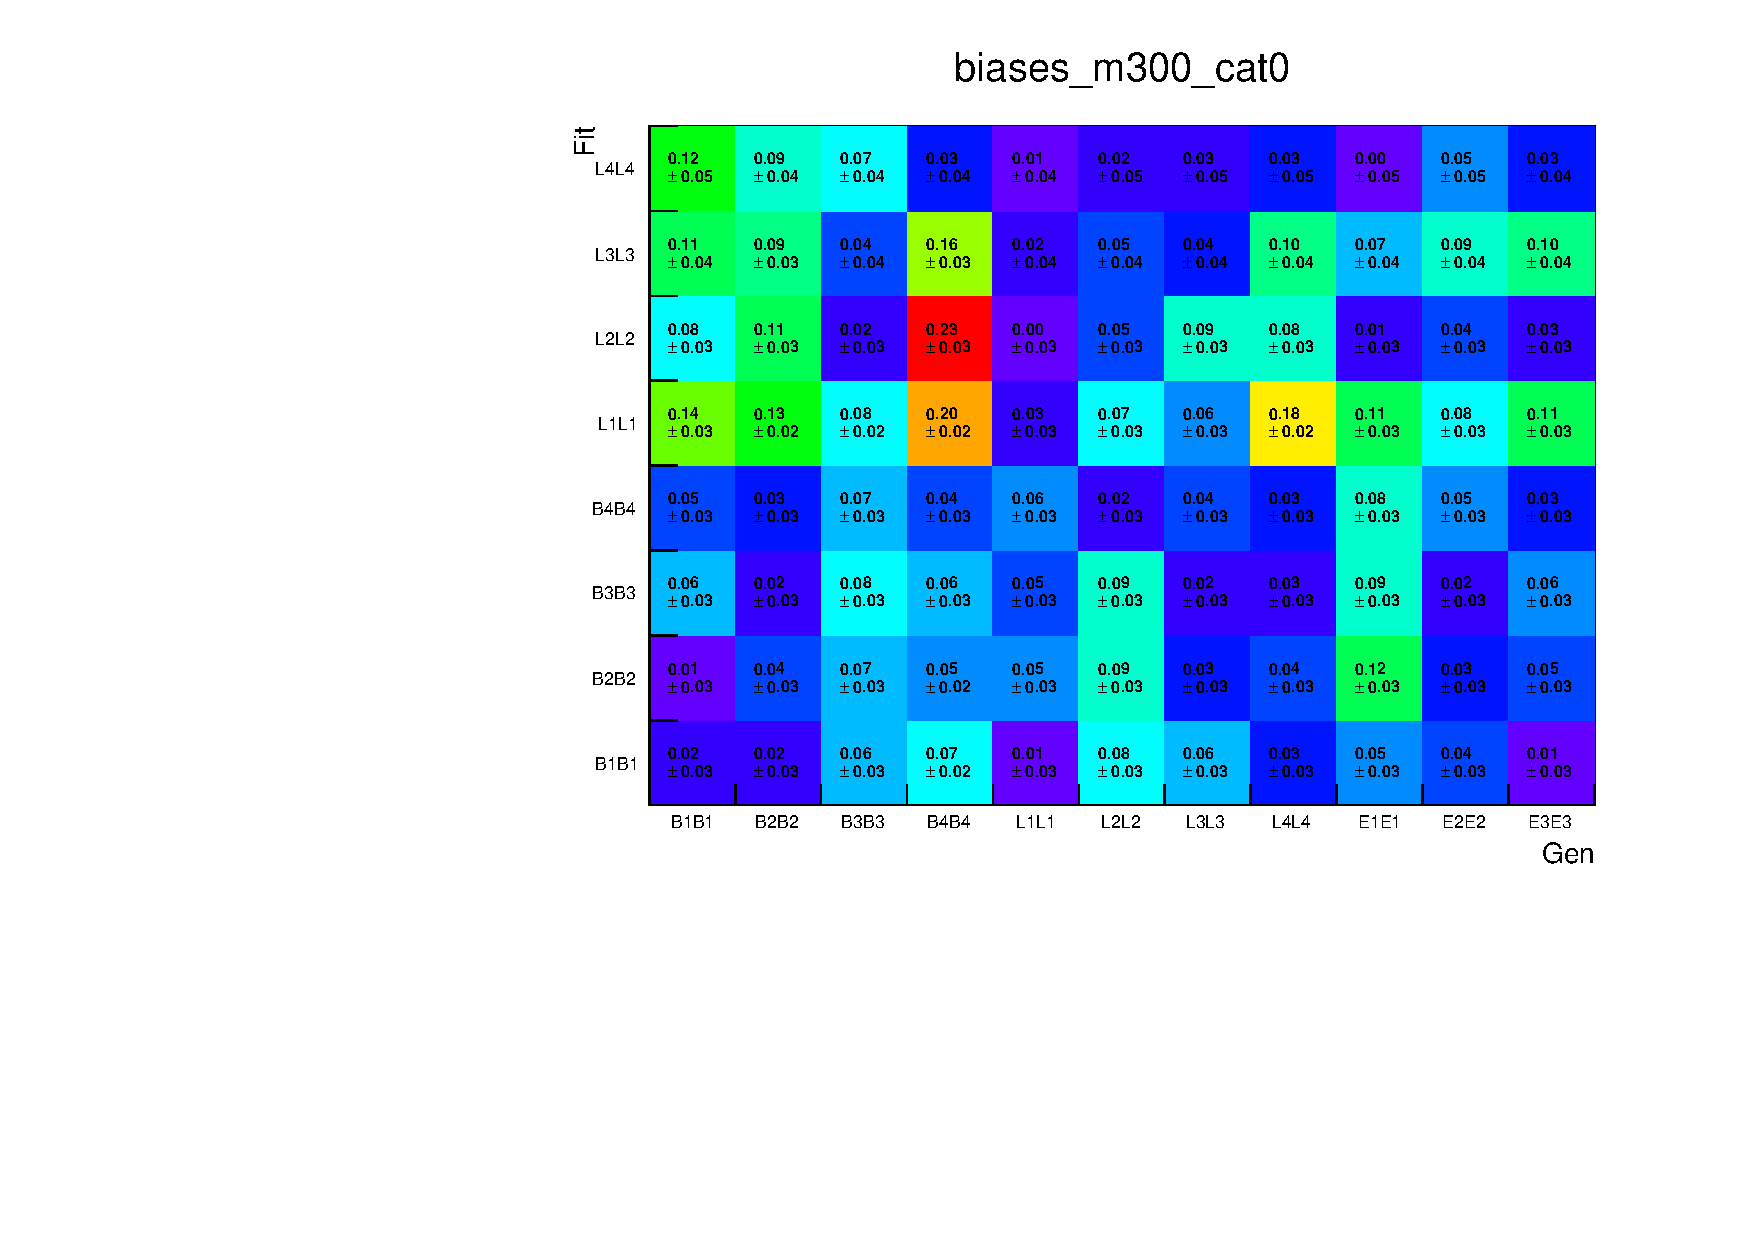
\includegraphics[width=0.48\textwidth]{figures/sec-bias/biases_m300_cat0.pdf}\hfil
  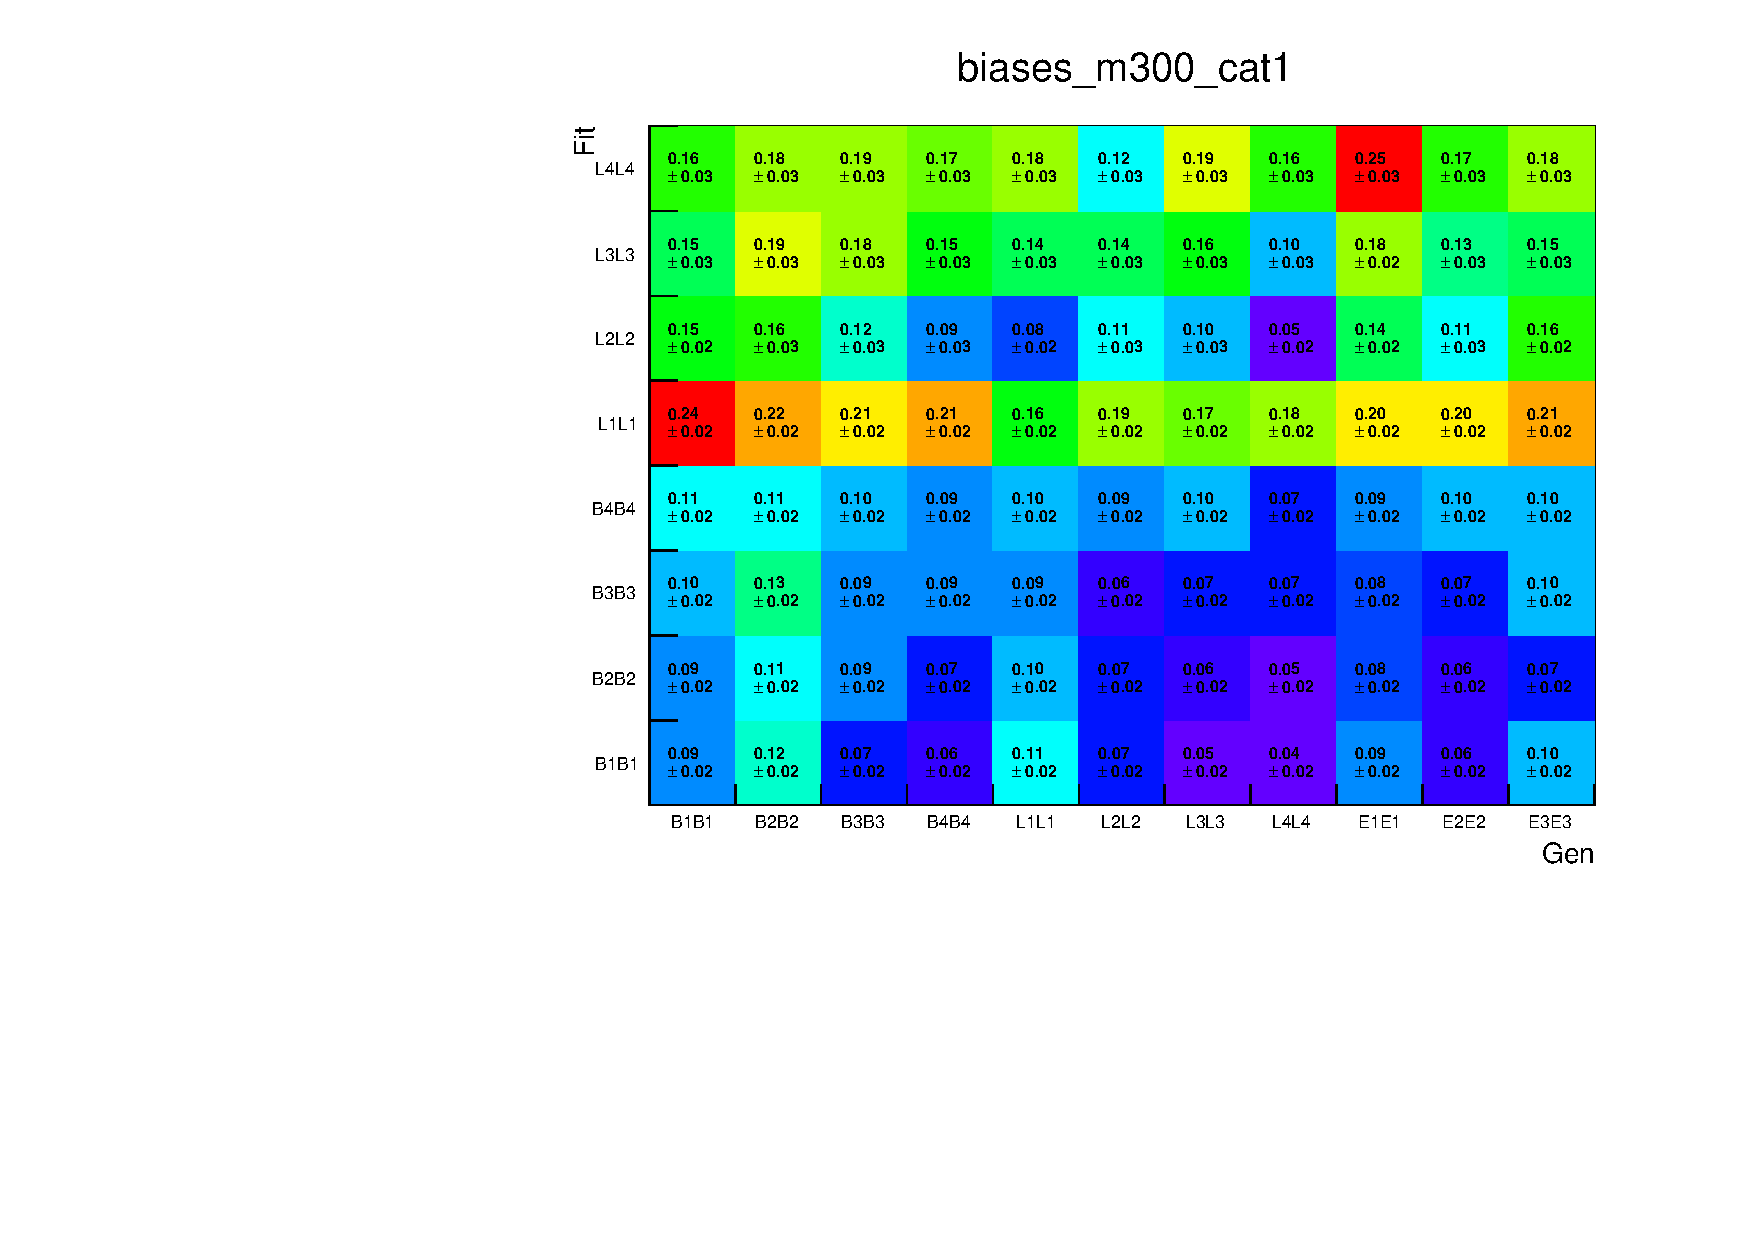
\includegraphics[width=0.48\textwidth]{figures/sec-bias/biases_m300_cat1.pdf}\hfil
  \caption{Biases measured in the 300 GeV resonant selection in the HPC (left) and MPC (right).}
  \label{fig:bkg_bias3}
\end{figure*}
\begin{figure*}[h]
  \centering
  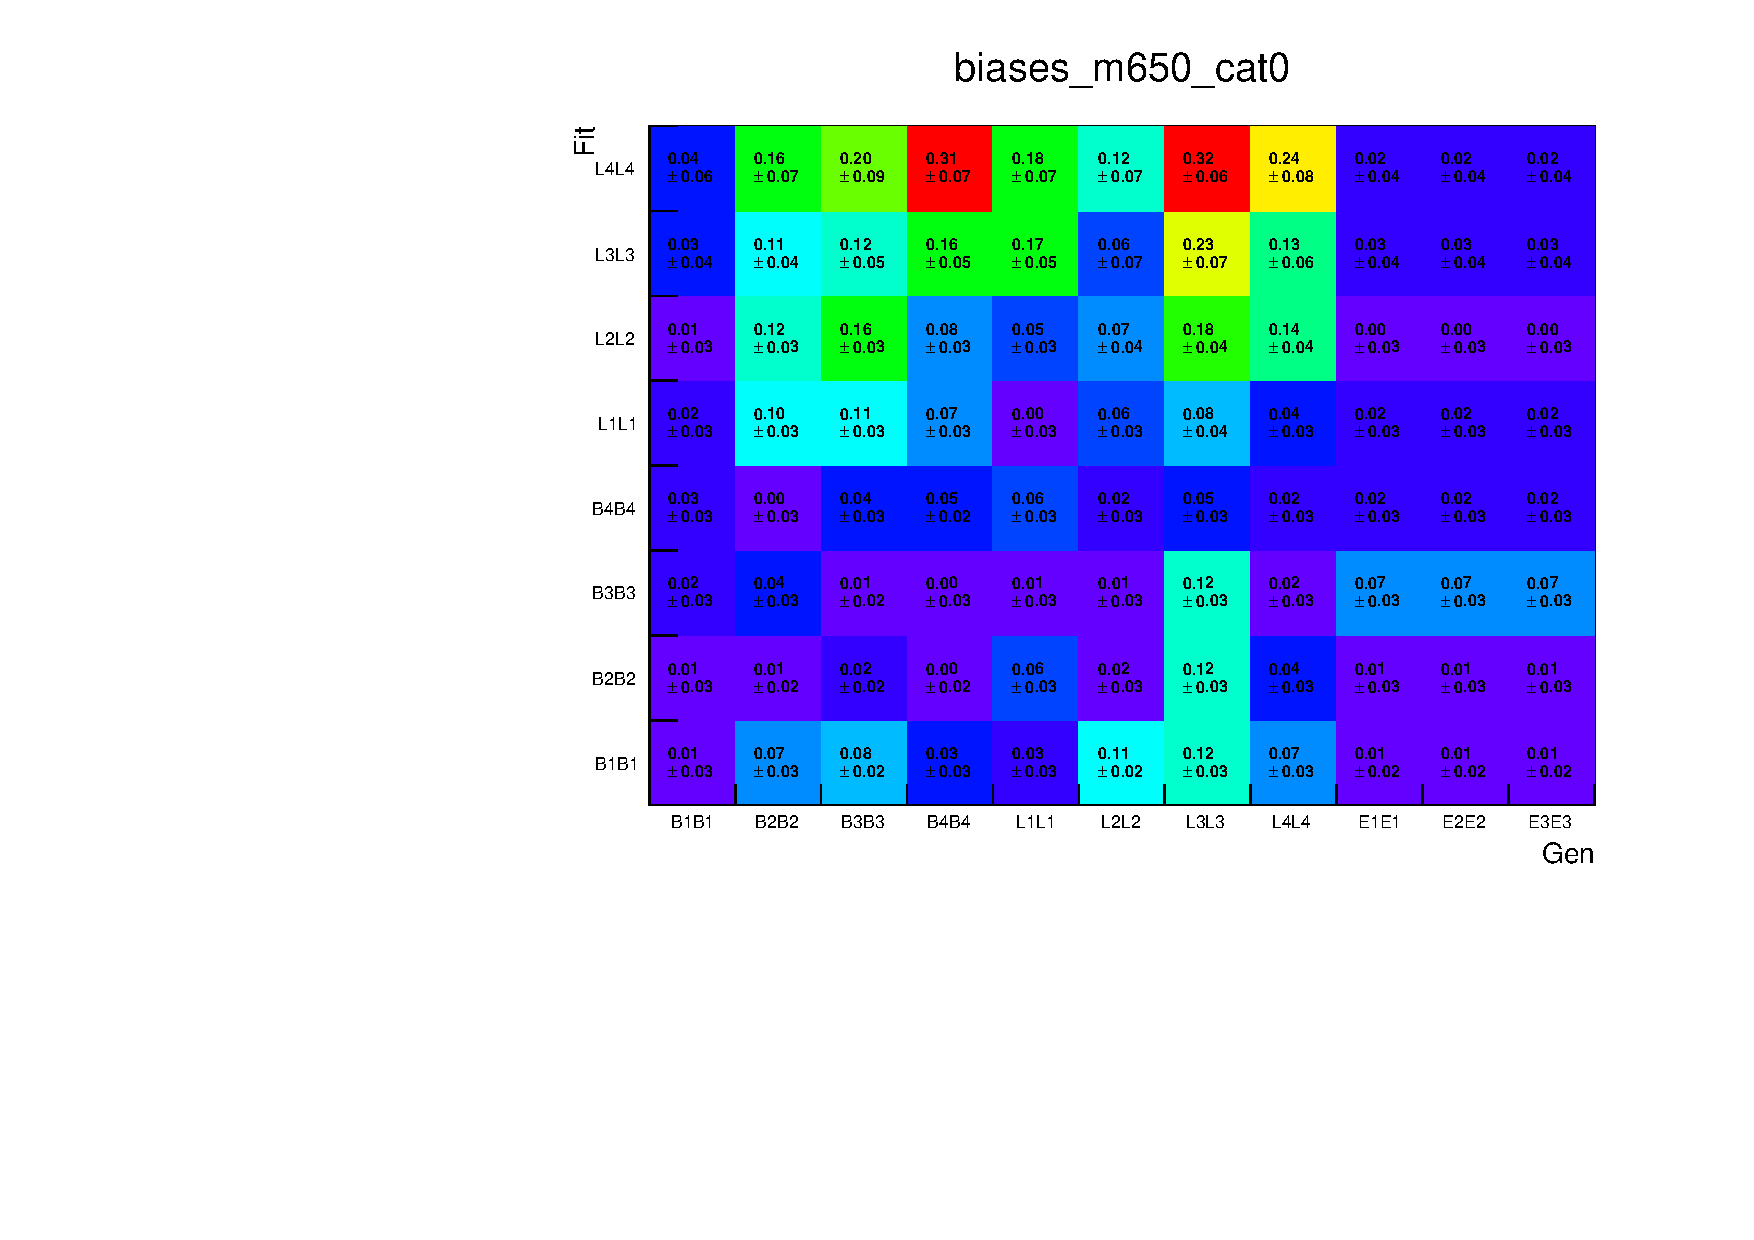
\includegraphics[width=0.48\textwidth]{figures/sec-bias/biases_m650_cat0.pdf}\hfil
  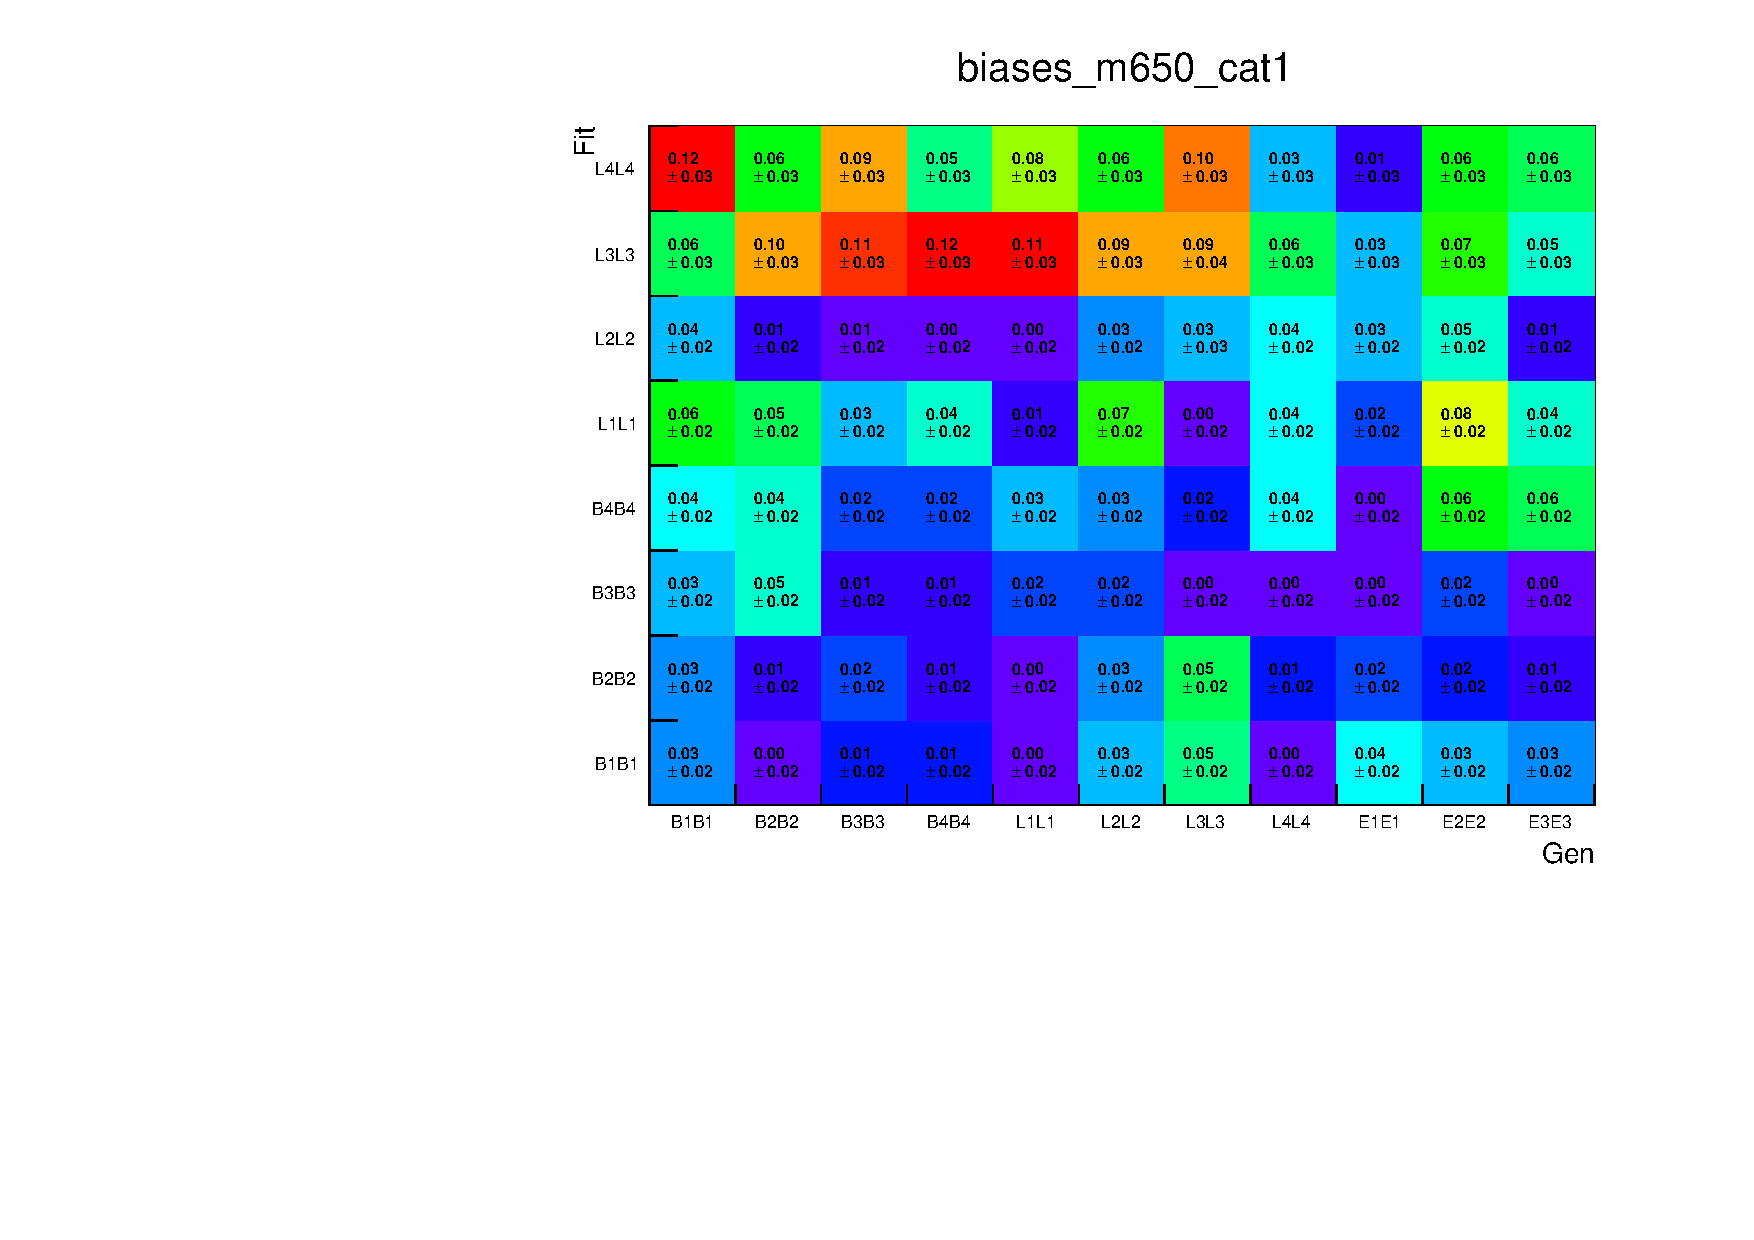
\includegraphics[width=0.48\textwidth]{figures/sec-bias/biases_m650_cat1.pdf}\hfil
  \caption{Biases measured in the 650 GeV resonant selection in the HPC (left) and MPC (right).}
  \label{fig:bkg_bias4}
\end{figure*}

\subsubsection{Goodness-of-Fit}

To check how well the background model fits the data, we perform a goodness-of-fit test in our blinded signal region.
The Kolmogorov-Smirnov (KS) test was chosen for its good performance on unbinned datasets, which is the case of this analysis.
Unfortunately, no 2-dimension unbinned KS tests are available with the current tools used in CMS.
The procedure taken was, then, to bin the 2D distribution with the analysis binning (40 bins in $\Mjj$ and 60 bins in $\Mgg$), making sure that the number of bins is much larger than the expected number of events (2400 bins is the case).
For the blinding procedure, we set the bins of the 2D histograms to 0 in the blinding region ($120 < \Mgg < 130$ GeV).
The requirement of the KS goodness-of-fit test is that the KS probability is >> 0.05, which is achieved for all the categories and signal regions: all KS probabilities are larger than 0.45.

\subsubsection{Correlation Studies}

Assuming that the overall 2D shape can be modeled by a 2D second order polynomial, the most general function can be constructed as:
\begin{equation}
f(x,y) = \sum_{i=0}^{i=2}\sum_{k=0}^{k=2}c_{ik}x^{i}y^{k},
\end{equation}
where, in our case, $x = \Mgg$ and $y = \Mjj$ or vice-versa. 
However, in our modeling, we assume $\Mgg$ and $\Mjj$ to be independent, therefore, our choice of model takes the form of:
\begin{equation}
g(x,y) = \left( \sum_{i=0}^{i=2} a_{i} x^{i}\right)\left( \sum_{k=0}^{k=2} a_{k} y^{k} \right).
\end{equation}
While the first equation has 9 degrees of freedom, the second only has 6. 
Therefore, by assuming our two parameters of interest to be independent, we lose three degrees of freedom in our model PDF. 
To study our sensitivity to these missing degrees of freedom, we construct a new PDF adding back three new parameters, namely:

\begin{eqnarray}
g_{corr}(x,y) &=& \left( \sum_{i=0}^{i=2} a_{i} x^{i}\right)\left( \sum_{k=0}^{k=2} a_{k} y^{k} \right) + \alpha\cdot\Mgg\cdot\Mjj \\
&+& \beta\cdot\Mgg^{2}\cdot\Mjj+ \omega\cdot\Mgg\cdot\Mjj^{2}.
\end{eqnarray}

We perform two tests with this PDF: 
\begin{itemize}
\item We generate Asimov datasets \cite{asimov_dataset} with $g_{corr}(x,y)$ for varying $(\alpha,\beta,\omega)$ and then fit it with $g(x,y)$. Then we check the residuals comparing $g_{corr}(x,y)$ and $g(x,y)$ assuming different normalizations (i.e., different number of expected background events).
\item We generate toy datasets with  $g_{corr}(x,y)$ for varying $(\alpha,\beta,\omega)$, with different values for the expected number of background events, with injected signal. Then we measure back the signal strength by using $g(x,y)$ and check the bias ($B = (\mu_{measured} - \mu_{true})/\sigma_{\mu}$).
\end{itemize}

In Figure \ref{fig:gcorr_alpha}, the 2D distributions of $g_{corr}(x,y)$ for different values of $\alpha$, where the change in correlation between $x$ and $y$ can be seen.  
In Figure \ref{fig:g_alpha}, the 2D distributions of $g(x,y)$ fitted to the Asimov datasets produced with  $g_{corr}(x,y)$ with different values of $\alpha$, where the change in correlation between $x$ and $y$ can be also be seen, albeit different from $g_{corr}(x,y)$. Therefore, we need to measure how sensitive we are to that difference. 
The first check is to calculate the 2D residuals, as was done for the signal correlation tests, between these two hypotheses, for different background normalizations. 
The residuals with the background normalized to 200 events can be seen in Figure \ref{fig:res_norm200}, and for 100000 events in Figure \ref{fig:res_norm100000}. 
While very little statistically significant deviation is seen for 200 background events, structures do start to appear with 100k background events, which is an expected behavior. 
This test was further performed with 10, 100, 500, 1000, 5000 background events, with conclusions similar to the 200 case. 
The test was also performed with varying $\beta$ and $\omega$ with similar conclusions. 

For the second test, instead of generating Asimov datasets, we generate toy MC for the different normalizations and $(\alpha,\beta,\omega)$ hypotheses. 
We then show the bias measurement for these different cases, in the hypothesis of varying $\alpha$, in Figure \ref{fig:corr_bias}. 
Since no bias larger than 14\% is seen, we don't include any systematics on the signal strength due to possible background correlations that are not modeled by our choice of PDF.

\begin{figure*}[h]
  \centering
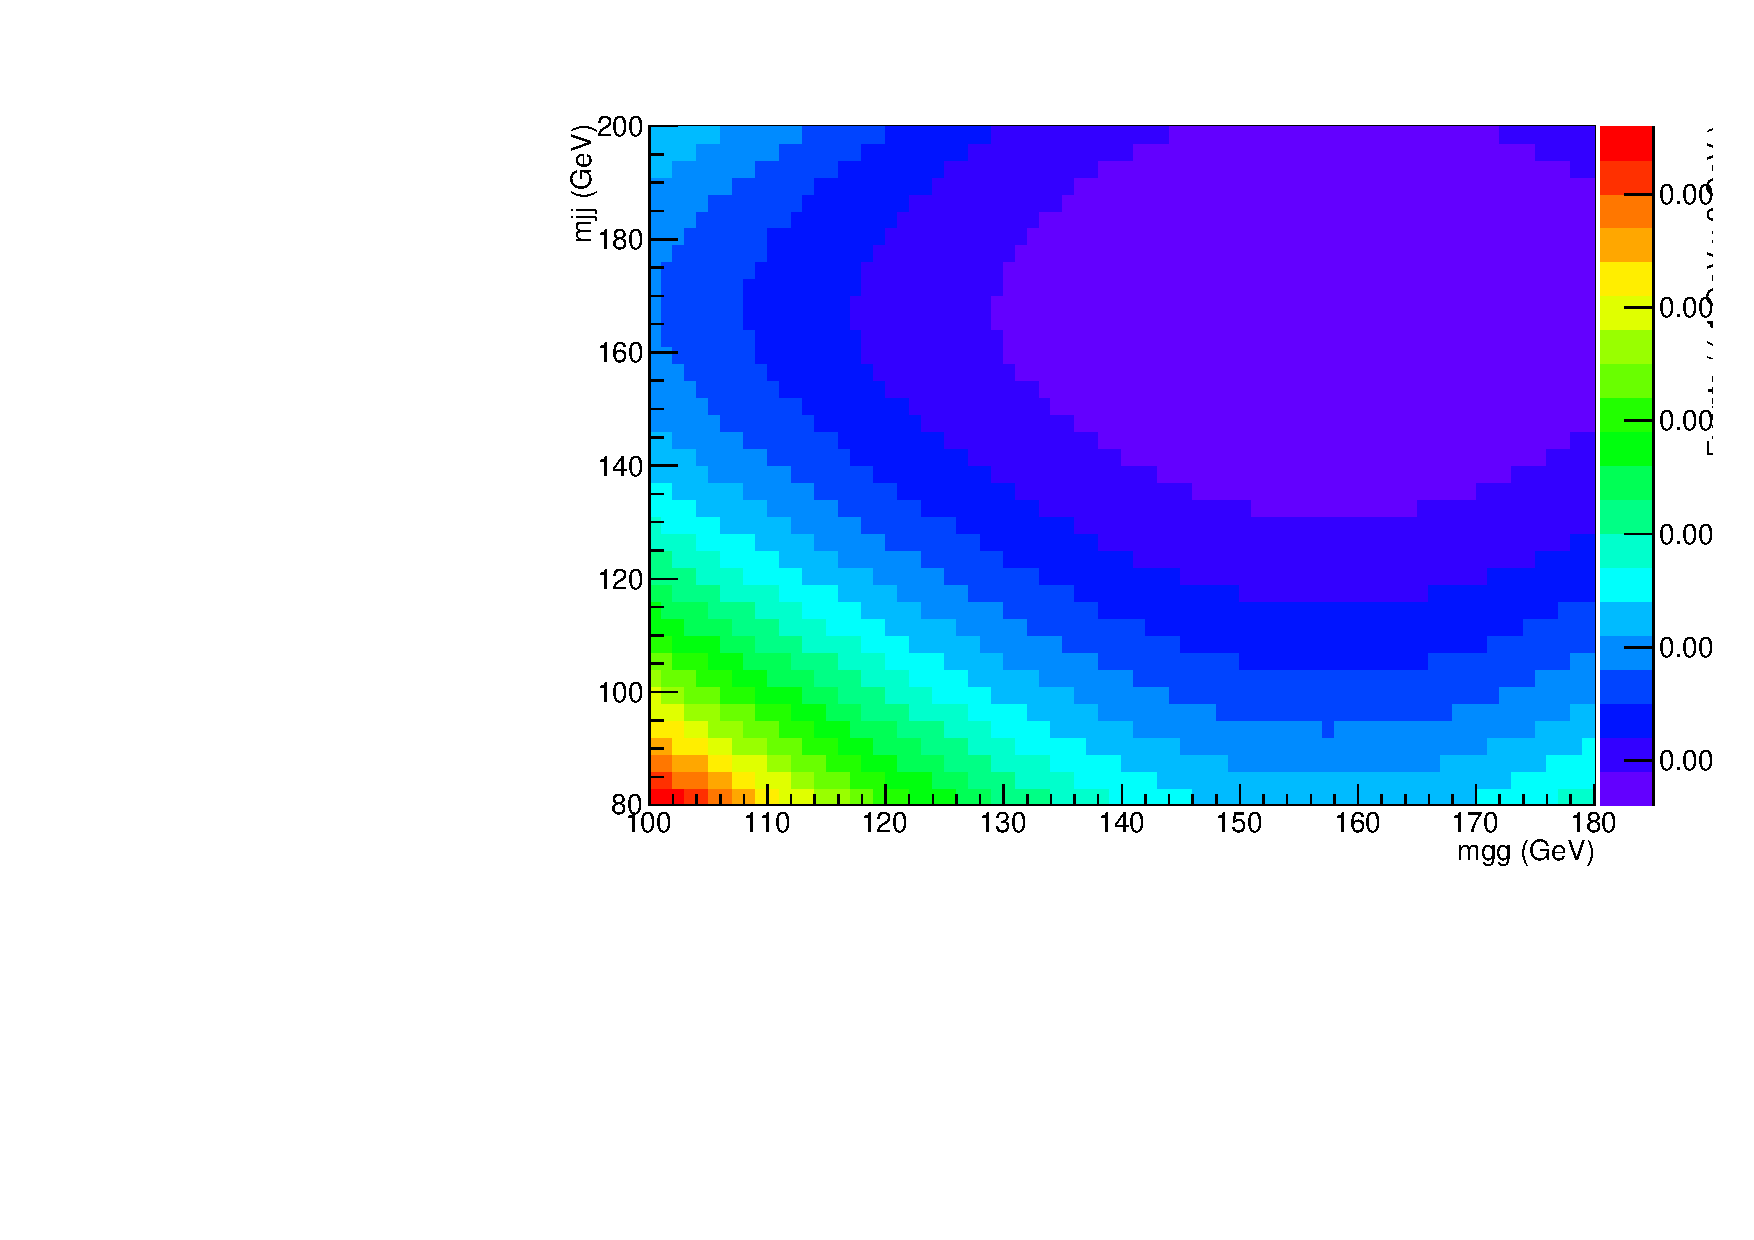
\includegraphics[width=0.32\textwidth]{figures/sec-background/correlation/res_th2F_exp_th2f_res_alpha_00_n005.pdf}
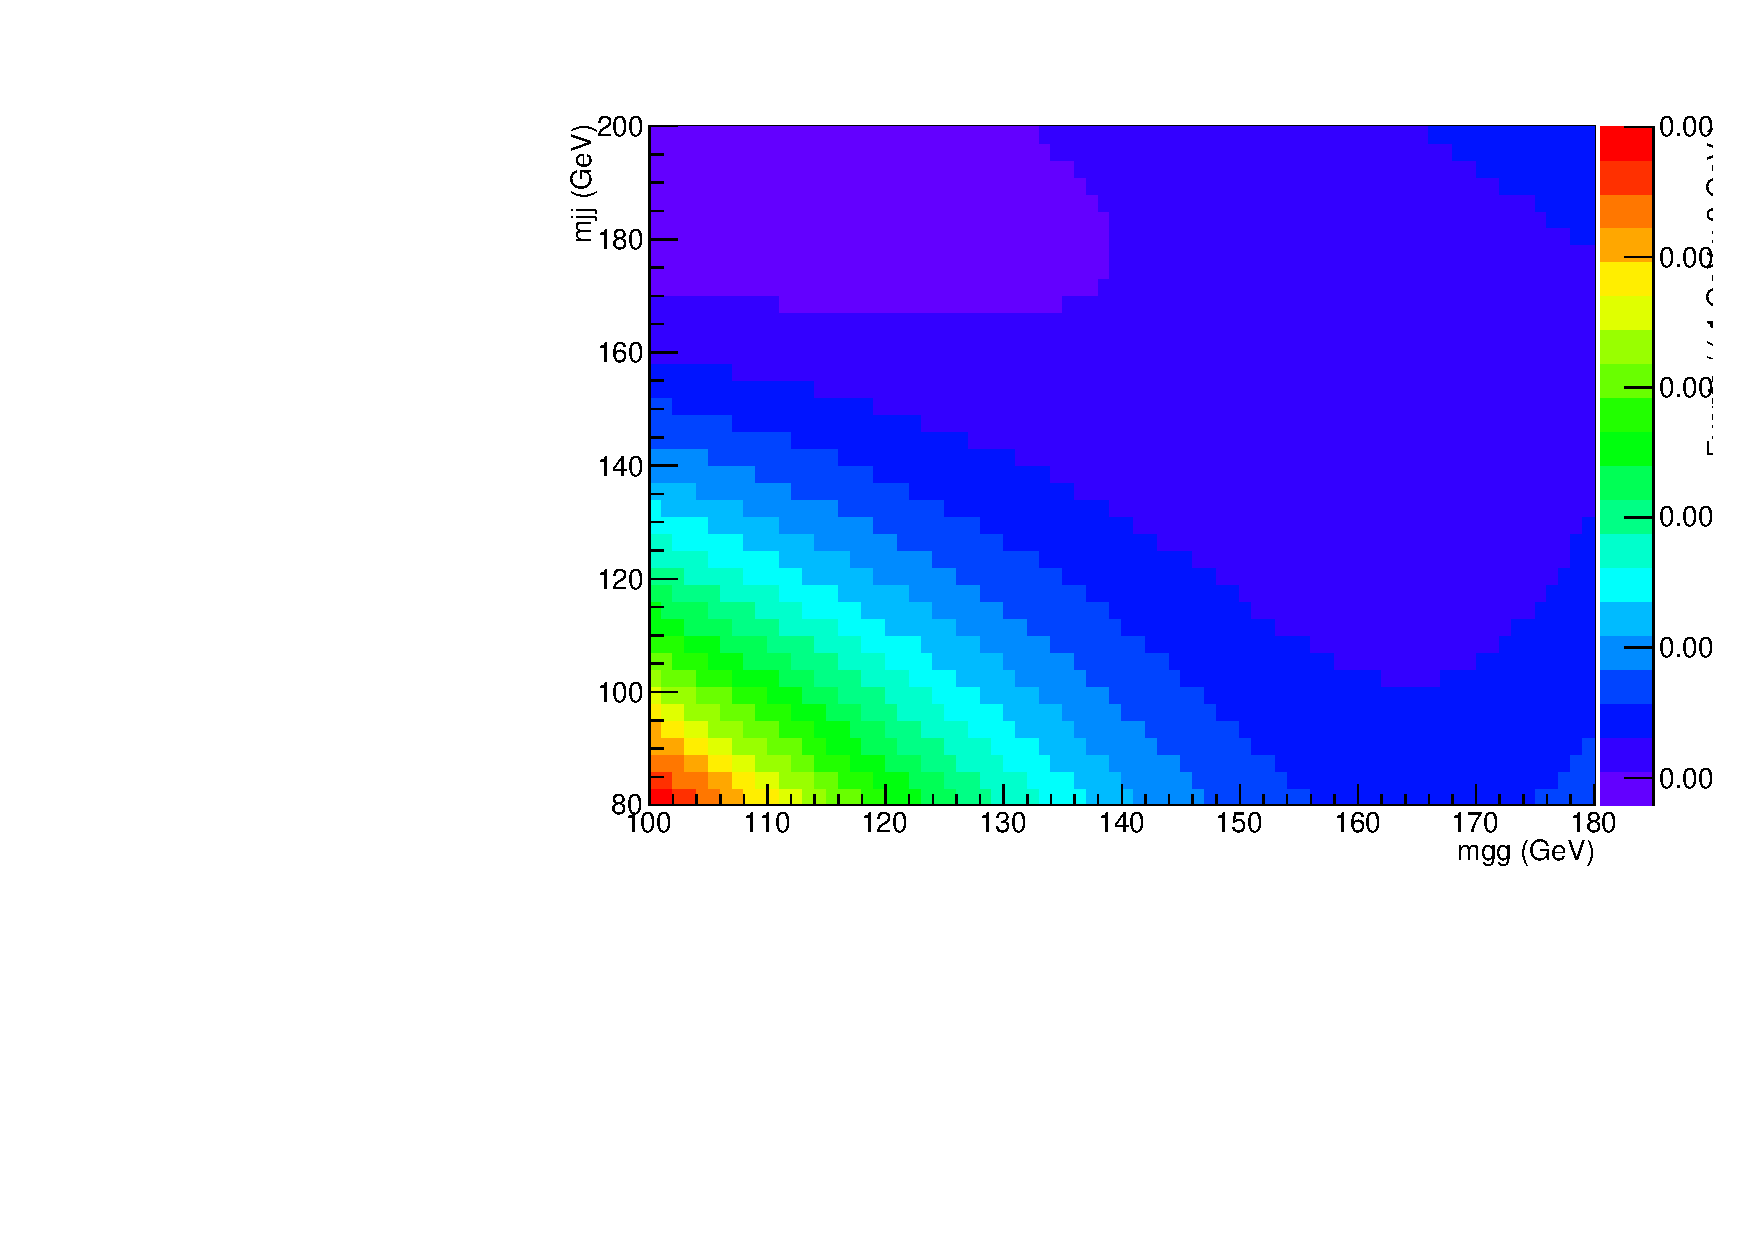
\includegraphics[width=0.32\textwidth]{figures/sec-background/correlation/res_th2F_exp_th2f_res_alpha_05_n005.pdf}
\includegraphics[width=0.32\textwidth]{figures/sec-background/correlation/res_th2F_exp_th2f_res_alpha_10_n005.pdf}
  \caption{2D distributions of $g_{corr}(M(\gamma\gamma),M(jj))$ with $\alpha = 0.0,\,0.5,\,1.0$, from left to right. }
  \label{fig:gcorr_alpha}
\end{figure*}

\begin{figure*}[h]
  \centering
\includegraphics[width=0.32\textwidth]{figures/sec-background/correlation/res_th2F_obs_th2f_res_alpha_00_n005.pdf}
\includegraphics[width=0.32\textwidth]{figures/sec-background/correlation/res_th2F_obs_th2f_res_alpha_05_n005.pdf}
\includegraphics[width=0.32\textwidth]{figures/sec-background/correlation/res_th2F_obs_th2f_res_alpha_10_n005.pdf}
  \caption{2D distributions of $g(M(\gamma\gamma),M(jj))$ fitted to the Asimov datasets produced with  $g_{corr}(x,y)$ with $\alpha = 0.0,\,0.5,\,1.0$, from left to right.}
  \label{fig:g_alpha}
\end{figure*}

\begin{figure*}[h]
  \centering
\includegraphics[width=0.32\textwidth]{figures/sec-background/correlation/res_th2F_res_th2f_res_alpha_00_n200.pdf}
\includegraphics[width=0.32\textwidth]{figures/sec-background/correlation/res_th2F_res_th2f_res_alpha_05_n200.pdf}
\includegraphics[width=0.32\textwidth]{figures/sec-background/correlation/res_th2F_res_th2f_res_alpha_10_n200.pdf}
  \caption{2D residuals comparing distributions of $g(M(\gamma\gamma),M(jj))$ fitted to the Asimov datasets produced with $g_{corr}(x,y)$ with $\alpha = 0.0,\,0.5,\,1.0$ and the dataset, from left to right. The background normalization is 200 events.}
  \label{fig:res_norm200}
\end{figure*}

\begin{figure*}[h]
  \centering
\includegraphics[width=0.32\textwidth]{figures/sec-background/correlation/res_th2F_res_th2f_res_alpha_00_n100000.pdf}
\includegraphics[width=0.32\textwidth]{figures/sec-background/correlation/res_th2F_res_th2f_res_alpha_05_n100000.pdf}
\includegraphics[width=0.32\textwidth]{figures/sec-background/correlation/res_th2F_res_th2f_res_alpha_10_n100000.pdf}
  \caption{2D residuals comparing distributions of $g(M(\gamma\gamma),M(jj))$ fitted to the Asimov datasets produced with $g_{corr}(M(\gamma\gamma),M(jj))$ with $\alpha = 0.0,\,0.5,\,1.0$ and the dataset, from left to right. The background normalization is 100k events.}
  \label{fig:res_norm100000}
\end{figure*}

\begin{figure*}[h]
  \centering
\includegraphics[width=0.9\textwidth]{figures/sec-background/CorrelationBias.pdf}
\caption{Relative bias on measuring the signal with $g(M(\gamma\gamma),M(jj))$ on toys created with $g_{corr}(M(\gamma\gamma),M(jj))$ with $\alpha$ from 0 to 1, for different background normalization hypotheses.}
\label{fig:corr_bias}
\end{figure*}

\subsection{Single Higgs Background Modeling}

Apart from the smoothly-falling background expected, depending on the integrated luminosity with which it is performed, the non-resonant analysis is also sensitive to the SM single Higgs production as a background process. 
In the resonant case, the mass window requirement reduces the single Higgs contributions to negligible levels, and therefore is not considered. 

The SM single Higgs background consists of the Higgs resonance in $\Mgg$ and a $\Mjj$ shape that depends on the production mechanism. 
For single Higgs produced via gluon fusion and vector boson fusion, the two extra jets will constitute a smoothly falling background, therefore, we model this contribution in the 2D $\Mgg:\Mjj$ plane with a product of a double sided Crystal-Ball (similar to our signal model)  and a second order Bernstein. 
For single Higgs produced in association with top quarks, bottom quarks and a vector boson, we are also able to model $\Mjj$ with a double-sided Crystal-Ball function, given the kinematic turn-on present in the first two cases, and the $V\rightarrow jj$ resonance in the latter.  
The Higgs model fits, in the High Purity category as an example, are shown in Figures \ref{fig:higgs_fit_ggh}, \ref{fig:higgs_fit_vbf}, \ref{fig:higgs_fit_vh}, \ref{fig:higgs_fit_bbh} and \ref{fig:higgs_fit_tth}.
The cross sections used for the SM single Higgs estimations are listed in Table \ref{tab:smsingleh}, along with their efficiencies in the four different non-resonant analysis categories. 

\begin{figure*}[h]
  \centering
\includegraphics[width=0.23\textwidth]{figures/sec-signals/HiggsShapes/ggh_HM_signal_fit_mgg_cat0.pdf}
%\includegraphics[width=0.23\textwidth]{figures/sec-signals/HiggsShapes/ggh_HM_signal_fit_mgg_cat1.pdf}
\includegraphics[width=0.23\textwidth]{figures/sec-signals/HiggsShapes/ggh_LM_signal_fit_mgg_cat0.pdf}
%\includegraphics[width=0.23\textwidth]{figures/sec-signals/HiggsShapes/ggh_LM_signal_fit_mgg_cat1.pdf}
\includegraphics[width=0.23\textwidth]{figures/sec-signals/HiggsShapes/ggh_HM_signal_fit_mjj_cat0.pdf}
%\includegraphics[width=0.23\textwidth]{figures/sec-signals/HiggsShapes/ggh_HM_signal_fit_mjj_cat1.pdf}
\includegraphics[width=0.23\textwidth]{figures/sec-signals/HiggsShapes/ggh_LM_signal_fit_mjj_cat0.pdf}
%\includegraphics[width=0.23\textwidth]{figures/sec-signals/HiggsShapes/ggh_LM_signal_fit_mjj_cat1.pdf}
  \caption{Higgs model fit to Higgs Monte Carlo (ggH) in the High Purity Category. From left to right: $\Mgg$ in high mass region, $\Mgg$ in low mass region, $\Mjj$ in high mass region, $\Mjj$ in low mass region.}
  \label{fig:higgs_fit_ggh}
\end{figure*}

\begin{figure*}[h]
  \centering
\includegraphics[width=0.23\textwidth]{figures/sec-signals/HiggsShapes/vbf_HM_signal_fit_mgg_cat0.pdf}
%\includegraphics[width=0.23\textwidth]{figures/sec-signals/HiggsShapes/vbf_HM_signal_fit_mgg_cat1.pdf}
\includegraphics[width=0.23\textwidth]{figures/sec-signals/HiggsShapes/vbf_LM_signal_fit_mgg_cat0.pdf}
%\includegraphics[width=0.23\textwidth]{figures/sec-signals/HiggsShapes/vbf_LM_signal_fit_mgg_cat1.pdf}
\includegraphics[width=0.23\textwidth]{figures/sec-signals/HiggsShapes/vbf_HM_signal_fit_mjj_cat0.pdf}
%\includegraphics[width=0.23\textwidth]{figures/sec-signals/HiggsShapes/vbf_HM_signal_fit_mjj_cat1.pdf}
\includegraphics[width=0.23\textwidth]{figures/sec-signals/HiggsShapes/vbf_LM_signal_fit_mjj_cat0.pdf}
%\includegraphics[width=0.23\textwidth]{figures/sec-signals/HiggsShapes/vbf_LM_signal_fit_mjj_cat1.pdf}
  \caption{Higgs model fit to Higgs Monte Carlo (VBF) in the High Purity Category. From left to right: $\Mgg$ in high mass region, $\Mgg$ in low mass region, $\Mjj$ in high mass region, $\Mjj$ in low mass region.}
  \label{fig:higgs_fit_vbf}
\end{figure*}

\begin{figure*}[h]
  \centering
\includegraphics[width=0.23\textwidth]{figures/sec-signals/HiggsShapes/vh_HM_signal_fit_mgg_cat0.pdf}
%\includegraphics[width=0.23\textwidth]{figures/sec-signals/HiggsShapes/vh_HM_signal_fit_mgg_cat1.pdf}
\includegraphics[width=0.23\textwidth]{figures/sec-signals/HiggsShapes/vh_LM_signal_fit_mgg_cat0.pdf}
%\includegraphics[width=0.23\textwidth]{figures/sec-signals/HiggsShapes/vh_LM_signal_fit_mgg_cat1.pdf}
\includegraphics[width=0.23\textwidth]{figures/sec-signals/HiggsShapes/vh_HM_signal_fit_mjj_cat0.pdf}
%\includegraphics[width=0.23\textwidth]{figures/sec-signals/HiggsShapes/vh_HM_signal_fit_mjj_cat1.pdf}
\includegraphics[width=0.23\textwidth]{figures/sec-signals/HiggsShapes/vh_LM_signal_fit_mjj_cat0.pdf}
%\includegraphics[width=0.23\textwidth]{figures/sec-signals/HiggsShapes/vh_LM_signal_fit_mjj_cat1.pdf}
  \caption{Higgs model fit to Higgs Monte Carlo (VH) in the High Purity Category. From left to right: $\Mgg$ in high mass region, $\Mgg$ in low mass region, $\Mjj$ in high mass region, $\Mjj$ in low mass region.}
  \label{fig:higgs_fit_vh}
\end{figure*}

\begin{figure*}[h]
  \centering
\includegraphics[width=0.23\textwidth]{figures/sec-signals/HiggsShapes/bbh_HM_signal_fit_mgg_cat0.pdf}
%\includegraphics[width=0.23\textwidth]{figures/sec-signals/HiggsShapes/bbh_HM_signal_fit_mgg_cat1.pdf}
\includegraphics[width=0.23\textwidth]{figures/sec-signals/HiggsShapes/bbh_LM_signal_fit_mgg_cat0.pdf}
%\includegraphics[width=0.23\textwidth]{figures/sec-signals/HiggsShapes/bbh_LM_signal_fit_mgg_cat1.pdf}
\includegraphics[width=0.23\textwidth]{figures/sec-signals/HiggsShapes/bbh_HM_signal_fit_mjj_cat0.pdf}
%\includegraphics[width=0.23\textwidth]{figures/sec-signals/HiggsShapes/bbh_HM_signal_fit_mjj_cat1.pdf}
\includegraphics[width=0.23\textwidth]{figures/sec-signals/HiggsShapes/bbh_LM_signal_fit_mjj_cat0.pdf}
%\includegraphics[width=0.23\textwidth]{figures/sec-signals/HiggsShapes/bbh_LM_signal_fit_mjj_cat1.pdf}
  \caption{Higgs model fit to Higgs Monte Carlo (bbH) in the High Purity Category. From left to right: $\Mgg$ in high mass region, $\Mgg$ in low mass region, $\Mjj$ in high mass region, $\Mjj$ in low mass region.}
  \label{fig:higgs_fit_bbh}
\end{figure*}

\begin{figure*}[h]
  \centering
\includegraphics[width=0.23\textwidth]{figures/sec-signals/HiggsShapes/tth_HM_signal_fit_mgg_cat0.pdf}
%\includegraphics[width=0.23\textwidth]{figures/sec-signals/HiggsShapes/tth_HM_signal_fit_mgg_cat1.pdf}
\includegraphics[width=0.23\textwidth]{figures/sec-signals/HiggsShapes/tth_LM_signal_fit_mgg_cat0.pdf}
%\includegraphics[width=0.23\textwidth]{figures/sec-signals/HiggsShapes/tth_LM_signal_fit_mgg_cat1.pdf}
\includegraphics[width=0.23\textwidth]{figures/sec-signals/HiggsShapes/tth_HM_signal_fit_mjj_cat0.pdf}
%\includegraphics[width=0.23\textwidth]{figures/sec-signals/HiggsShapes/tth_HM_signal_fit_mjj_cat1.pdf}
\includegraphics[width=0.23\textwidth]{figures/sec-signals/HiggsShapes/tth_LM_signal_fit_mjj_cat0.pdf}
%\includegraphics[width=0.23\textwidth]{figures/sec-signals/HiggsShapes/tth_LM_signal_fit_mjj_cat1.pdf}
  \caption{Higgs model fit to Higgs Monte Carlo (ttH) in the High Purity Category. From left to right: $\Mgg$ in high mass region, $\Mgg$ in low mass region, $\Mjj$ in high mass region, $\Mjj$ in low mass region.}
  \label{fig:higgs_fit_tth}
\end{figure*}



\begin{table}[h]
{\small
\centering
    \begin{tabular}{c | c | c | c | c | c }
     & Cross section (pb) & HM-HPC (\%) & HM-MPC (\%) & LM-HPC (\%) & LM-MPC (\%)\\ \hline
    ggH & 44.14 & $0.029\pm0.0017$ & $0.148\pm0.0038$ & $0.033\pm0.0018$ & $0.151\pm0.0039$  \\
    VBF & 3.7820 & $0.038\pm0.001$ & $0.239\pm0.0025$ & $0.048\pm0.0011$ & $0.242\pm0.0025$ \\
    VH & 2.257 & $0.271\pm0.0038$ & $0.748\pm0.0063$ & $0.367\pm0.0044$ & $0.962\pm0.0071$ \\
    $b\bar{b}$H & 0.488  & $0.0297\pm0.0035$  & $0.262\pm0.010$  & $1.02\pm0.020$  &  $2.59\pm0.032$ \\
    $t\bar{t}$H & 0.5071 & $3.41\pm0.027$ & $3.69\pm0.029$ & $8.38\pm0.042$ & $8.17\pm0.042$ 
    \end{tabular}
\caption{SM single Higgs cross sections at 13 TeV with their respective selection efficiencies for the four different non-resonant analysis categories: High Mass-High Purity, High Mass-Medium Purity, Low Mass-High Purity and Low Mass-Medium Purity categories.}
}
\label{tab:smsingleh}
\end{table}
